% !TeX spellcheck = en_GB, gr_GR

\newglossaryentry{minimum}
{
	name=minimum,
	description={Given a set of real numbers, the minimum\index{minimum} is the smallest of those numbers.},
	first={minimum},text={minimum}
}


\newglossaryentry{maximum}
{name=maximum,
 description={Given a set of real numbers, the maximum\index{maximum} is the largest of those numbers.},
 first={maximum},text={maximum}
}

\newglossaryentry{discrepancy}
{name=discrepancy,
	description={
		Consider\index{discrepancy} an \gls{fl} application with \gls{netdata} 
		represented by an \gls{empgraph}. \gls{fl} methods use a discrepancy measure 
		to compare \gls{hypothesis} maps from local models at nodes $\nodeidx,\nodeidx'$ 
		connected by an edge in the \gls{empgraph}.},
	first={discrepancy},text={discrepancy}
}



\newglossaryentry{hfl}
{name={horizontal \gls{fl}},description=
	{Horizontal \gls{fl}\index{horizontal FL} uses \gls{localdataset}s constituted by different
	   \gls{datapoint}s but uses the same \gls{feature}s to characterize them \cite{HFLChapter2020}.
		For example, weather forecasting uses a network of spatially distributed
		weather (observation) stations. Each weather station measures the
		same quantities such as daily temperature, air pressure and precipitation.
		However, different weather stations measure the characteristics or
		\gls{feature}s of different spatiotemporal regions. Each spatio-temporal region 
		represents an individual \gls{datapoint}, are characterized by the same \gls{feature}s 
		(e.g., daily temperature or air pressure).},
	first={horizontal \gls{fl}},text={horizontal \gls{fl}}
} 

\newglossaryentry{dimred}
{name={dimensionality reduction},
	description={Dimensionality reduction\index{dimensionality reduction} methods 
		map (typically many) raw \gls{feature}s to a (relatively small) set of 
		new \gls{feature}s. These methods can be used to visualize \gls{datapoint}s 
		by learning two \gls{feature}s that can be used as the coordinates of a 
		depiction in a \gls{scatterplot}.}, first={dimensionality reduction},text={dimensionality reduction}
} 

\newglossaryentry{featlearn}
{name={feature learning},
	description={Consider an ML application with \gls{datapoint}s characterized by 
		\emph{raw} \gls{feature}s $\featurevec \in \featurespace$. Feature learning\index{feature learning} 
		refers to the task of learning a map 
		$$\featuremapvec: \featurespace \rightarrow \featurespace': \featurevec \mapsto \featurevec',$$ 
		that reads in raw \gls{feature}s $\featurevec \in \featurespace$ of a \gls{datapoint} and delivers new 
		\gls{feature}s $\featurevec' \in \featurespace'$ from a new \gls{featurespace} $\featurespace'$. 
		Different \gls{feature} learning methods are obtained for different design 
		choices of $\featurespace,\featurespace'$, a \gls{hypospace} $\hypospace$ 
		of potential maps $\featuremapvec$ and quantitative measure of the usefulness of 
		a specific $\featuremapvec \in \hypospace$. For example, \gls{pca} 
		uses $\featurespace \defeq \mathbb{R}^{\dimlocalmodel}$, $\featurespace' \defeq \mathbb{R}^{\dimlocalmodel'}$ 
		with $\dimlocalmodel' < \dimlocalmodel$ and \gls{hypospace} 
		$$\hypospace\defeq \big\{ \featuremapvec: \mathbb{R}^{\dimlocalmodel}
		\!\rightarrow\! \mathbb{R}^{\dimlocalmodel'}\!:\!\featurevec'\!\defeq\!\mF \featurevec \mbox{ with some } \mF \!\in\! \mathbb{R}^{\dimlocalmodel' \times \dimlocalmodel} \big\}.$$ \Gls{pca} measures the usefulness of a specific map $\featuremapvec(\featurevec)= \mF \featurevec$ 
	by the minimum linear reconstruction error incurred on a \gls{dataset}, 
$$ \min_{\mG \in \mathbb{R}^{\dimlocalmodel \times \dimlocalmodel'}} \sum_{\sampleidx=1}^{\samplesize} \normgeneric{\mG \mF \featurevec^{(\sampleidx)} - \featurevec^{(\sampleidx)}}{2}^{2}.$$ }, 
	first={feature learning},text={feature learning}
} 

\newglossaryentry{autoencoder}
{name={\foreignlanguage{greek}{αυτοκωδικοποιητής}},
	description={\foreignlanguage{greek}{Ένας αυτοκωδικοποιητής} 
	(autoencoder)\index{\foreignlanguage{greek}{αυτοκωδικοποιητής}} \foreignlanguage{greek}{είναι μία 
	μέθοδος μηχανικής μάθησης που μαθαίνει μαζί μία αντιστοίχιση κωδικοποίησης} 
	$\hypothesis(\cdot) \in \hypospace$ \foreignlanguage{greek}{και μία αντιστοίχιση αποκωδικοποίησης} 
	$\hypothesis^{*}(\cdot) \in \hypospace^{*}$. \foreignlanguage{greek}{Είναι μία περίπτωση} 
	\gls{erm} \foreignlanguage{greek}{που χρησιμοποιεί μία} \gls{loss} \foreignlanguage{greek}{υπολογιζόμενη από το σφάλμα ανακατασκευής}
	$\featurevec - \hypothesis^{*}\big(  \hypothesis \big( \featurevec \big) \big)$.},
	first={autoencoder},text={autoencoder}
}

\newglossaryentry{vfl}
{name={vertical \gls{fl}},description=
	{Vertical \gls{fl}\index{vertical FL} uses \gls{localdataset}s that are constituted 
	 by the same \gls{datapoint}s but characterizing them with different \gls{feature}s \cite{VFLChapter}. 
     For example, different healthcare providers might all contain information 
     about the same population of patients. However, different healthcare providers 
     collect different measurements (blood values, electrocardiography, lung X-ray) 
     for the same patients.},
	first={vertical \gls{fl}},text={vertical \gls{fl}}
} 

\newglossaryentry{interpretability}
{name={interpretability},description=
		{An ML method is interpretable\index{interpretability} for a specific user if 
			they can anticipate the \gls{prediction}s delivered by the method well. 
			The notion of interpretability can be made precise using quantitative 
			measures of the uncertainty about the \gls{prediction}s \cite{JunXML2020}.},
		first={interpretability},text={interpretability}
}

\newglossaryentry{multitask learning}
{name={multitask learning},description=
	{Multitask learning\index{multitask learning} aims at leveraging relations between 
	 different \gls{learningtask}s. Consider two \gls{learningtask}s obtained from the 
	 same \gls{dataset} of webcam snapshots. The first task is to predict the presence 
	 of a human, while the second is the predict the presence of a car. It might be useful 
	 to use the same \gls{deepnet} structure for both tasks and only allow the weights of 
	 the final output layer to be different.},
	first={multitask learning},text={multitask learning}
}

\newglossaryentry{learningtask}
{name={learning task},description=
	{Consider\index{learning task} a \gls{dataset} $\dataset$ constituted by several \gls{datapoint}s, each of them 
	 characterized by \gls{feature}s $\featurevec$. For example, the \gls{dataset} $\dataset$ 
	 might be constituted by the images of a particular database. Sometimes it might be useful 
	 to represent a \gls{dataset} $\dataset$, along with the choice of \gls{feature}s, by a \gls{probdist} $p(\featurevec)$. 
	 A learning task associated with $\dataset$ consists of a specific 
	 choice for the \gls{label} of a \gls{datapoint} and the corresponding \gls{labelspace}. 
	 Given a choice for the \gls{lossfunc} and \gls{model}, a learning task gives rise to an 
	 instance of \gls{erm}. Thus, we could define a learning task also via an instance of \gls{erm}, i.e., 
	 via an objective function.  Note that, for the same \gls{dataset}, we obtain different learning tasks by using 
	 different choices for the \gls{feature}s and \gls{label} of a \gls{datapoint}. These learning 
	 tasks are related, as they are based on the same \gls{dataset}, and solving them jointly 
	 (via multitask learning methods) is typically preferable over solving them separately \cite{Caruana:1997wk,JungGaphLassoSPL,CSGraphSelJournal}.},
	first={learning task},text={learning task}
}

\newglossaryentry{explainability}
{name={explainability},description=
		{We\index{explainability} define the (subjective) explainability of an ML method 
			as the level of simulatability \cite{Colin:2022aa} of the \gls{prediction}s 
			delivered by an ML system to a human user. Quantitative measures for the 
			(subjective) explainability of a trained \gls{model} can be constructed by 
			comparing its \gls{prediction}s with the \gls{prediction}s provided by a user 
			on a \gls{testset} \cite{Zhang:2024aa,Colin:2022aa}. Alternatively, we can use 
			\gls{probmodel}s for \gls{data} and measure the explainability of a trained ML model 
			via the conditional (differential) entropy of its \gls{prediction}s, given the user \gls{prediction}s \cite{JunXML2020,Chen2018}. 
		},
		first={explainability},text={explainability}
	}

\newglossaryentry{linmodel}{name={linear model},
	description={Consider\index{linear model}  \gls{datapoint}s, each characterized by a numeric \gls{feature} 
		vector $\featurevec \in \mathbb{R}^{\featuredim}$. A linear \gls{model} is 
		a \gls{hypospace} which consists of all linear maps, 
	\begin{equation} 
		\label{equ_def_lin_model_hypspace}
		\linmodel{\nrfeatures} \defeq \left\{ \hypothesis(\featurevec)= \weights^{T} \featurevec: \weights \in \mathbb{R}^{\nrfeatures} \right\}. 
	\end{equation} 
	Note that \eqref{equ_def_lin_model_hypspace} defines an entire family of \gls{hypospace}s, which is 
	parameterized by the number $\nrfeatures$ of \gls{feature}s that are linearly combined to form the 
	\gls{prediction} $\hypothesis(\featurevec)$. The design choice of $\nrfeatures$ is guided by \gls{compasp} 
	(smaller $\nrfeatures$ means less computation), \gls{statasp} (increasing $\nrfeatures$ might 
	reduce \gls{prediction} error) and \gls{interpretability}. A linear \gls{model} using few carefully chosen 
	\gls{feature}s tends to be considered more interpretable \cite{Ribeiro2016,rudin2019stop}.}, 
   first={linear model},text={linear model}}
	
	
\newglossaryentry{gradstep}{name={gradient step},description={Given a \gls{differentiable} 
		real-valued function $f(\cdot): \mathbb{R}^{\nrfeatures} \rightarrow \mathbb{R}$ 
		 and a vector $\weights \in \mathbb{R}^{\nrfeatures}$, the \gls{gradient} step\index{gradient step} 
		 updates $\weights$ by adding the scaled negative \gls{gradient} $\nabla f(\weights)$ to obtain 
		 the new vector (see Fig.\ \ref{fig_basic_GD_step_single})
		 \begin{equation}
		 \label{equ_def_gd_basic} 
		\widehat{\weights}  \defeq \weights - \lrate \nabla f(\weights).
		\end{equation} 
		Mathematically, the gradient step is a (typically non-linear) operator $\mathcal{T}^{(f,\lrate)}$ 
		that is parametrized by the function $f$ and the \gls{stepsize} $\lrate$. 
		\begin{figure}[htbp]
			\begin{center}
				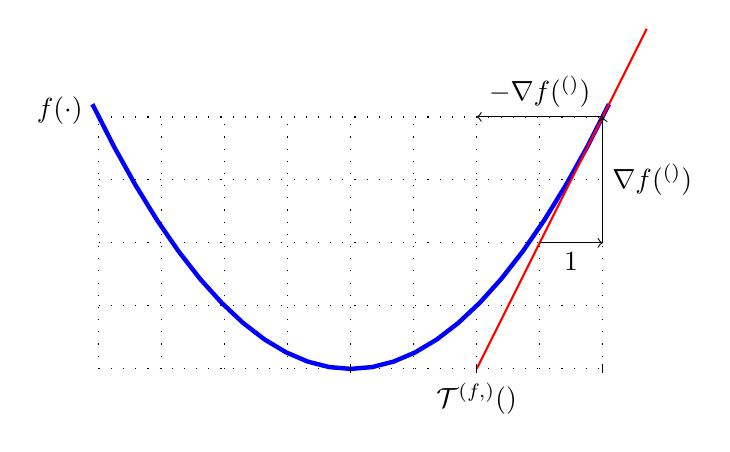
\begin{tikzpicture}[scale=0.8]
					\draw[loosely dotted] (-4,0) grid (4,4);
					\draw[blue, ultra thick, domain=-4.1:4.1] plot (\x,  {(1/4)*\x*\x});
					\draw[red, thick, domain=2:4.7] plot (\x,  {2*\x - 4});
					\draw[<-] (4,4) -- node[right] {$\nabla f(\weights^{(\itercntr)})$} (4,2);
					\draw[->] (4,4) -- node[above] {$-\lrate \nabla f(\weights^{(\itercntr)})$} (2,4);
					\draw[<-] (4,2) -- node[below] {$1$} (3,2) ;
					%\draw[->] (-4.25,0) -- (4.25,0) node[right] {$a$};
					\node[left] at (-4.1, 4.1) {$f(\cdot)$}; 
					\draw[shift={(0,0)}] (0pt,2pt) -- (0pt,-2pt) node[below] {$\overline{\weights}$};
					\draw[shift={(4,0)}] (0pt,2pt) -- (0pt,-2pt) node[below] {$\weights$};
					\draw[shift={(2,0)}] (0pt,2pt) -- (0pt,-2pt) node[below] {$\mathcal{T}^{(f,\lrate)}(\weights)$};
				\end{tikzpicture}
			\end{center}
			\caption{The basic gradient step \eqref{equ_def_gd_basic} maps a given vector $\weights$ 
			to the updated vector $\weights'$. It defines an operator 
			$\mathcal{T}^{(f,\lrate)}(\cdot): \mathbb{R}^{\nrfeatures} \rightarrow \mathbb{R}^{\nrfeatures}:
			 \weights \mapsto \widehat{\weights}$.}
			\label{fig_basic_GD_step_single}
		\end{figure}
		Note that the gradient step \eqref{equ_def_gd_basic} optimizes locally - 
		in a neighbourhood whose size is determined by the \gls{stepsize} $\lrate$ - a linear approximation 
		to the function $f(\cdot)$. A natural generalization of \eqref{equ_def_gd_basic} is to locally 
		optimize the function itself - instead of its linear approximation - 
		\begin{align} 
		\label{equ_approx_gd_step}
		\widehat{\weights} = \argmin_{\weights' \in \mathbb{R}^{\dimlocalmodel}} f(\weights')\!+\!(1/\lrate)\normgeneric{\weights-\weights'}{2}^2. 
		\end{align}
		We intentionally use the same symbol $\lrate$ for the parameter in \eqref{equ_approx_gd_step} 
		as we used for the step size in \eqref{equ_def_gd_basic}. The larger we choose $\lrate$ in 
		\eqref{equ_approx_gd_step}, the more progress the update will make towards reducing the 
		function value $f(\widehat{\weights})$. Note that, much like the gradient step \eqref{equ_def_gd_basic}, 
		also the update \eqref{equ_approx_gd_step} defines a (typically non-linear) operator 
		that is parametrized by the function $f(\cdot)$ and the parameter $\lrate$. For a \gls{convex} function 
		$f(\cdot)$, this operator is known as the \gls{proxop} of $f(\cdot)$ \cite{ProximalMethods}. 
		},first={gradient step},text={gradient step}}
	

\newglossaryentry{proxop}{name={proximal operator},description={Given\index{proximal operator} a \gls{convex} 
		function $f(\weights')$, we define its proximal operator as \cite{ProximalMethods,Bauschke:2017} 
		$$\proximityop{f(\cdot)}{\weights}{\rho}\defeq \argmin_{\weights' \in \mathbb{R}^{\dimlocalmodel}} \bigg[ f(\weights')\!+\!(\rho/2) \normgeneric{\weights- \weights'}{2}^{2}\bigg] \mbox{ with } \rho > 0. $$ 
		As illustrated in Figure \ref{fig_proxoperator_opt}, evaluating the proximal operator 
		amounts to minimizing a penalized variant of $f(\weights')$. The penalty term is the 
		scaled squared Euclidean distance to a given vector $\weights$ (which is the input to the proximal operator). 
		%\Gls{convex} functions for which the proximal operator can be computed efficiently 
		%is sometimes referred to as \emph{proximable} or \emph{simple} \cite{Condat2013}. 
		The proximal operator can be interpreted as a generalization of the \gls{gradstep}, which is defined 
		for a \gls{smooth} \gls{convex} function $f(\weights')$. Indeed, taking a 
		\gls{gradstep} with \gls{stepsize} $\lrate$ at current vector $\weights$ 
		is the same as applying the \gls{proxop} of the function $\tilde{f}(\weights')= \big( \nabla f(\weights)\big)^{T} (\weights'-\weights)$ 
		and using $\rho=1/\lrate$.
			\begin{figure}
			\begin{center}
				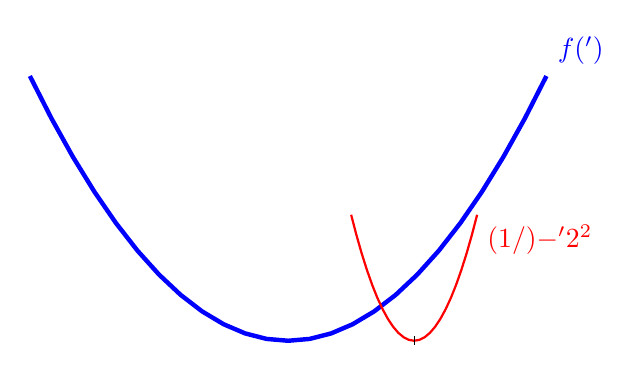
\begin{tikzpicture}[scale=0.8]
					% Original quadratic function
					\draw[blue, ultra thick, domain=-4.1:4.1] plot (\x, {(1/4)*\x*\x}) node[above right] {$f(\weights')$};		
					% Quadratic function with larger curvature, centered at w = 2
					\draw[red, thick, domain=1:3] plot (\x, {2*(\x - 2)*(\x - 2)}) node[below right] {$(1/\lrate)\normgeneric{\weights-\weights'}{2}^{2}$};
					% Axes
					% Minimum point of second curve
					\draw[shift={(2,0)}] (0pt,2pt) -- (0pt,-2pt) node[below] {$\weights$};
					%\node at (2,0.5) [anchor=north] {$\weights$};
				\end{tikzpicture}
			\end{center}
			\caption{A generalized gradient step updates a vector $\weights$ by minimizing a penalized version 
				of the function $f(\cdot)$. The penalty term is the squared Euclidean distance between the optimization 
				variable $\weights'$ and the given vector $\weights$.	\label{fig_proxoperator_opt}}
		\end{figure}
		},first={proximal operator},text={proximal operator}}

\newglossaryentry{proximable}{name={proximable},description={A\index{proximable} 
		\gls{convex} function for which the \gls{proxop} can be computed efficiently is 
		sometimes referred to as \emph{proximable} or \emph{simple} \cite{Condat2013}.},first={proximable},text={proximable}}


\newglossaryentry{connected}{name ={connected graph}, description={An\index{connected graph} 
		undirected graph $\graph=\pair{\nodes}{\edges}$ is connected\index{connected graph} if 
		it does not contain a (non-empty) subset $\nodes' \subset \nodes$ with no edges leaving 
		$\nodes'$.}, first={connected},text={connected}}

\newglossaryentry{mvndist}{name ={multivariate normal distribution}, description={The\index{multivariate normal distribution} 
		multivariate normal distribution $\mvnormal{\vm}{\mC}$ is an 
		important family of \gls{probdist}s for a continuous \gls{rv} $\featurevec \in \mathbb{R}^{\nrfeatures}$ \cite{BertsekasProb,GrayProbBook,Lapidoth09}. 
		This family is parameterized by the mean $\vm$ and \gls{covmtx} $\mC$ of $\featurevec$. 
		If the \gls{covmtx} is invertible, the \gls{probdist} of $\featurevec$ is 
		$$p(\featurevec) \propto \exp\bigg(-(1/2) \big( \featurevec - \vm \big)^{T} \mC^{-1} \big( \featurevec - \vm \big) \bigg).$$}, first={multivariate normal distribution},text={multivariate normal distribution}}

\newglossaryentry{statasp}{name ={statistical aspects}, description={By statistical aspects\index{statistical aspects} 
		of an ML method, we refer to (properties of) the \gls{probdist} of its output 
		under a \gls{probmodel} for the data fed into the method.},first={statistical aspects},text={statistical aspects}}

\newglossaryentry{compasp}{name ={computational aspects}, description={By computational 
		aspects\index{computational aspects} of an ML method, we mainly refer to the computational 
		resources required for its implementation. For example, if an ML method uses iterative 
		optimization techniques to solve \gls{erm}, then its computational aspects include (i) how 
		many arithmetic operations are needed to implement a single iteration (\gls{gradstep}) 
		and (ii) how many iterations are needed to obtain useful \gls{modelparams}. One important 
		example of an iterative optimization technique is \gls{gd}.}, first={computational aspects},text={computational aspects}}

\newglossaryentry{zerooneloss}{name={$0/1$ \gls{loss}},
	description={The $0/1$ \gls{loss}\index{$0/1$ loss} $\lossfunc{\pair{\featurevec}{\truelabel}}{\hypothesis}$ 
		measures the quality of a \gls{classifier} $\hypothesis(\featurevec)$ that delivers a \gls{prediction} $\predictedlabel$ (e.g., 
	via thresholding \eqref{equ_def_threshold_bin_classifier}) for the \gls{label} $\truelabel$ of a \gls{datapoint} with \gls{feature}s 
	$\featurevec$. 
	It is equal to $0$ if the \gls{prediction} is correct, i.e., 
	$\lossfunc{\pair{\featurevec}{\truelabel}}{\hypothesis}=0$ when $\predictedlabel=\truelabel$. It is 
	equal to $1$ if the \gls{prediction} is wrong, $\lossfunc{\pair{\featurevec}{\truelabel}}{\hypothesis}=1$ 
	when $\predictedlabel\neq\truelabel$.},
	sort=zerooneloss, 
    first={$0/1$ \gls{loss}},text={$0/1$ \gls{loss}}}

\newglossaryentry{probability}{name={probability},
	description={We\index{probability} assign a probability value, typically chosen in the 
		interval $[0,1]$, to each event that might occur in a random experiment \cite{KallenbergBook,BertsekasProb,BillingsleyProbMeasure,HalmosMeasure}.},first={probability},text={probability}}
	
\newglossaryentry{underfitting}{name={underfitting},description={Consider\index{underfitting} 
		an ML method that uses \gls{erm} to learn a \gls{hypothesis} with the minimum \gls{emprisk} 
		on a given \gls{trainset}. Such a method is \emph{underfitting} the \gls{trainset} if it is 
		not able to learn a \gls{hypothesis} with sufficiently small \gls{emprisk} on the \gls{trainset}. 
		If a method is underfitting it will typically also not be able to learn a \gls{hypothesis} with 
		a small \gls{risk}.},first={underfitting},text={underfitting}}

\newglossaryentry{overfitting}{name={overfitting},description={Consider\index{overfitting} an 
		ML method that uses \gls{erm} to learn a \gls{hypothesis} with the minimum \gls{emprisk} on 
		a given \gls{trainset}. Such a method is \emph{overfitting} the \gls{trainset} if it learns 
		a \gls{hypothesis} with small \gls{emprisk} on the \gls{trainset} but a significantly larger \gls{loss} outside the \gls{trainset}.},first={overfitting},text={overfitting}}

\newglossaryentry{gdpr}{name={General Data Protection Regulation},description={
			The\index{GDPR} General Data Protection Regulation (GDPR) was enacted by the European Union (EU), 
			effective from May 25, 2018 \cite{GDPR2016}. It safeguards the privacy and data rights of individuals in the EU. 
			The GDPR has significant implications for how data is collected, stored, and used in ML 
			applications. Key provisions include:
			\begin{itemize}
				\item \Gls{dataminprinc}: ML systems should only use the necessary amount of personal 
				\gls{data} for their purpose.
				\item Transparency and \Gls{explainability}: ML systems should enable their users to 
				understand how they make decisions that impact them.
				\item Data Subject Rights: Including the rights to access, rectify, and delete 
				personal data, as well as to object to automated decision-making and profiling.
				\item Accountability: Organizations must ensure robust data security and demonstrate 
				compliance through documentation and regular audits.
			\end{itemize}
			}, 
	first={general data protection regulation (GDPR) },text={GDPR}}
	
\newglossaryentry{gaussrv}{name={Gaussian random variable},description={
		A \index{Gaussian random variable} standard Gaussian \gls{rv} is a 
		real-valued random variable $x$ with \gls{pdf} \cite{papoulis,BertsekasProb,GrayProbBook}
		\begin{equation}
			\nonumber
			p(x) = \frac{1}{\sqrt{2\pi}} \exp^{-x^2/2}. 
		\end{equation}
		Given a standard Gaussian \gls{rv} $x$, we can construct a general Gaussian \gls{rv} $x'$ with 
		mean $\mu$ and variance $\sigma^2$ via $x' \defeq \sigma (x+\mu)$. The \gls{probdist} of a 
		Gaussian \gls{rv} is referred to as normal distribution, denoted $\mathcal{N}(\mu,\sigma)$.  \\ 
		A Gaussian random vector $\featurevec \in \mathbb{R}^{\featuredim}$ with 
		\gls{covmtx} $\mathbf{C}$ and mean ${\bm \mu}$ can be constructed via 
		$\featurevec \defeq \mathbf{A} \big( \vz + {\bm \mu} \big)$. Here, $\mA$ 
		is any matrix that satisfies $\mA\mA^{T} = \mC$ and $\vz \defeq \big( z_{1},\ldots,z_{\featuredim} \big)^{T}$
		is a vector whose entries are \gls{iid} standard Gaussian \gls{rv}s $z_{1},\ldots,z_{\featuredim}$. Gaussian 
		random processes generalize Gaussian random vectors by applying linear 
		transformations to infinite sequences of standard Gaussian \gls{rv}s \cite{Rasmussen2006Gaussian}.\\
		Gaussian \gls{rv}s are widely used \gls{probmodel}s for the statistical analysis of 
		machine learning methods. Their significance arises partly from the central limit theorem 
		which states that the average of an increasing number of independent \gls{rv}s (not necessarily Gaussian themselves) 
		converges to a Gaussian \gls{rv} \cite{ross2013first}. 
},first={Gaussian RV},text={Gaussian RV}}

\newglossaryentry{trustworthiness}{name={trustworthiness},description=
	{Besides the \gls{compasp} and \gls{statasp}, a third main design aspect of 
	ML methods is their trustworthiness\index{trustworthy AI} \cite{pfau2024engineeringtrustworthyaideveloper}. 
		The European Union has put forward seven key requirements (KRs) for trustworthy 
		AI (that typically build on ML methods)
	\cite{ALTAIEU}: {\bf KR1 - Human Agency and Oversight}, {\bf KR2 - Technical Robustness and Safety}, 
	{\bf KR3 - Privacy and Data Governance}, {\bf KR4 - Transparency}, {\bf KR5 - Diversity Non-Discrimination and Fairness}, 
	{\bf KR6 Societal and Environmental Well-Being}, and {\bf KR7 - Accountability}. 
	},first={trustworthiness},text={trustworthiness}}

\newglossaryentry{sqerrloss}{name={squared error loss},description={The squared 
		error\index{squared error loss} \gls{loss} measures the prediction error of a 
		\gls{hypothesis} $\hypothesis$ when predicting a numeric \gls{label} $\truelabel \in \mathbb{R}$ 
		from the \gls{feature}s $\featurevec$ of a \gls{datapoint}. It is 
	defined as 
\begin{equation} 
	\nonumber
%	\label{equ_squared_loss_gls}
	\lossfunc{(\featurevec,\truelabel)}{\hypothesis} \defeq \big(\truelabel - \underbrace{\hypothesis(\featurevec)}_{=\predictedlabel} \big)^{2}. 
\end{equation} 
},first={squared error loss},text={squared error loss}}


 \newglossaryentry{projection}{name={projection}, 
       description={Consider\index{projection} a subset $\paramspace \subseteq \mathbb{R}^{\dimlocalmodel}$ of 
	   the $\dimlocalmodel$-dimensional \gls{euclidspace}. We define the projection $\projection{\paramspace}{\weights}$
	   of a vector $\weights \in \mathbb{R}^{\dimlocalmodel}$ onto $\paramspace$ as
		\begin{equation} 
   	    \label{equ_def_proj_generic}
  	     \projection{\paramspace}{\weights} = \argmin_{\weights' \in \paramspace} \normgeneric{\weights - \weights'}{2}. 
         \end{equation}
		 In other words, $\projection{\paramspace}{\weights}$ is the vector in $\paramspace$ which is closest to $\weights$. 
		 The projection is only well-defined for subsets $\paramspace$ for which the above minimum exists \cite{BoydConvexBook}.},
		 first={projection},text={projection}}


\newglossaryentry{projgd}{name={projected gradient descent (projected GD)},
description={Consider a \gls{erm}-based method, using a parametrized \gls{model} with  
\gls{paramspace} $\paramspace \subseteq \mathbb{R}^{\dimlocalmodel}$. Even if 
the \gls{objfunc} of \gls{erm} is smooth, we cannot use basic \gls{gd} as 
it does not take into account contraints on the optimization variable (the \gls{modelparams}). 
Projected\index{projected gradient descent (projected GD)} \gls{gd} 
extends basic \gls{gd} to handle constraints on the optimization variable (\gls{modelparams}). 
A single iteration of projected \gls{gd} consists of first taking a \gls{gradstep} 
and then projecting the result back into the \gls{paramspace}.
\begin{figure}[htbp]
	\begin{center}
		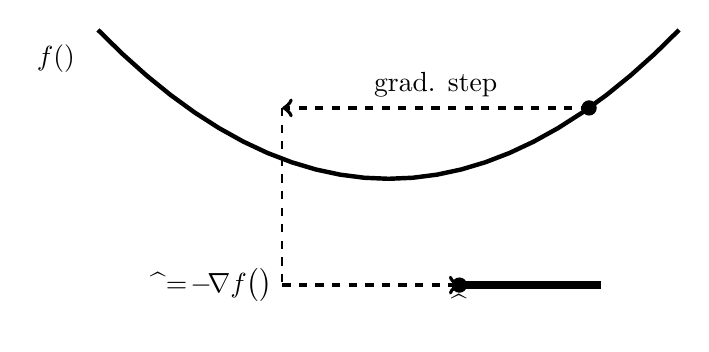
\begin{tikzpicture}[scale=0.9]
			\node [right] at (-5.1,1.7) {$f(\weights)$} ;
			\draw[ultra thick, domain=-4.1:4.1] plot (\x,  {(1/8)*\x*\x});
		%	\draw[dashed, thick, domain=1:3.6] plot (\x,  {\x - 1}) node[right] {$ f\big(\weights^{(\itercntr)}\big)\!+\!\big(\weights\!-\!\weights^{(\itercntr)}\big)^{T} \nabla f\big(\weights^{(\itercntr)}\big)$};
			\draw [fill] (2.83,1) circle [radius=0.1] node[right] {$\weights$};
			\draw[line width =0.5mm,dashed,->] (2.83,1) -- node[midway,above] {grad. step} (-1.5,1);
			\draw[line width =0.2mm,dashed] (-1.5,1) --(-1.5,-1.5)  node [below, left]{$\widehat{\weights}=\weights\!-\!\lrate \nabla f\big(\weights\big)$} ;
			\draw[line width =0.5mm,dashed,->] (-1.5,-1.5)  -- node[midway,above] {} (1,-1.5) ; 
			\draw [fill] (1,-1.5) circle [radius=0.1] node[below] {$\projection{\paramspace}{\widehat{\weights}}$};
			\draw[line width=1mm] (1,-1.5) -- (3,-1.5) node[midway, above] {$\paramspace$};
		\end{tikzpicture}
		\vspace*{-5mm}
	\end{center}
	\caption{\Gls{projgd} augments a basic \gls{gradstep} with a projection back 
	onto the constraint set $\paramspace$.}
	\label{fig_projected_GD}
\end{figure}},first={projected \gls{gd}},text={projected \gls{gd}}}

\newglossaryentry{diffpriv}
{name=differential privacy (DP),
  description={
  	Consider some ML method $\algomap$ that reads in a \gls{dataset} (e.g., the \gls{trainset} 
  	used for \gls{erm}) and delivers some output $\algomap(\dataset)$. The output 
  	could be either the learnt \gls{modelparams} or the \gls{prediction}s for specific \gls{datapoint}s. 
  	Differential privacy is a precise measure of privacy leakage incurred by revealing the 
  	output. Roughly speaking, an ML method is differentially private if the \gls{probdist} 
  	of the output $\algomap(\dataset)$ does not change too much if the \gls{sensattr} 
  	of one \gls{datapoint} in the \gls{trainset} is changed. Note that differential privacy 
  	builds on a \gls{probmodel} for an ML method, i.e., we interpret its output $\algomap(\dataset)$ 
  	as the \gls{realization} of a \gls{rv}. The randomness in the output can be ensured 
  	by intentionally adding the \gls{realization} of an auxiliary \gls{rv} (\emph{noise}) to 
  	the output of the ML method.}, 
	first = {differential privacy (DP)}, text={DP} 
}

\newglossaryentry{privprot}
{name=privacy protection,
     description={Consider\index{privacy protection} some ML method $\algomap$ that reads 
	 in a \gls{dataset} $\dataset$ and delivers some output $\algomap(\dataset)$. The output 
	 could be the learnt \gls{modelparams} $\widehat{\weights}$ or the \gls{prediction} 
	 $\learnthypothesis(\featurevec)$ obtained for a specific \gls{datapoint} with \gls{feature}s 
	 $\featurevec$. Many important ML applications involve \gls{datapoint}s 
		representing humans. Each \gls{datapoint} is characterized by \gls{feature}s $\featurevec$, 
		potentially a \gls{label} $\truelabel$ and a \gls{sensattr} $\sensattr$ (e.g., a recent medical diagnosis). 
		Roughly speaking, \gls{privprot} means that it should be impossible to infer, from the output $\algomap(\dataset)$, 
		any of the \gls{sensattr}s of \gls{datapoint}s in $\dataset$. Mathematically, \gls{privprot} requires non-invertibility 
		of the map $\algomap(\dataset)$. In general, just making $\algomap(\dataset)$ non-invertible 
		is typically insufficient for \gls{privprot}. We need to make $\algomap(\dataset)$ sufficiently non-invertible. 
	}, 
	first = {privacy protection}, text={privacy protection} 
}

\newglossaryentry{privleakage}
{
	name=privacy leakage,
	description={Consider\index{privacy leakage} an ML application that processes a 
	\gls{dataset} $\dataset$ and delivers some output, such as the predictions 
	obtained for new \gls{datapoint}s. Privacy leakage arises 
	if the output carries information about a private (sensitive) \gls{feature} of 
	a \gls{datapoint} (which might be a human) of $\dataset$. Based on a \gls{probmodel} 
	for the data generation, we can measure the privacy leakage via the \gls{mutualinformation} 
	between the output and the senstive \gls{feature}. Another quantitative measure of privacy leakage 
	is \gls{diffpriv}. The relations between different measures of privacy leakage have been 
	studied in \cite{InfThDiffPriv}. 
	}, 
	first = {privacy leakage}, text={privacy leakage} 
}



\newglossaryentry{probmodel}
{
	name=probabilistic model,
	description={A probabilistic model\index{probabilistic model} interprets \gls{datapoint}s 
		as \gls{realization}s of \gls{rv}s with a joint \gls{probdist}. This joint \gls{probdist} typically 
		involves parameters which have to be manually chosen or learnt via statistical inference 
		methods such as \gls{ml} \cite{LC}. }, 
	first = {probabilistic model}, text={probabilistic model} 
}



\newglossaryentry{mean}
{
	name=mean,
	description={The\index{mean} expectation $\expect \{ \featurevec \}$ of a numeric \gls{rv} $\featurevec$.}, 
		first = {mean}, text={mean} 
}

\newglossaryentry{variance}
{
	name={variance},
	description={The\index{variance} variance of a real-valued \gls{rv} $\feature$ is defined as the expectation 
		$\expect\big\{ \big( x - \expect\{x \} \big)^{2} \big\}$ of the squared difference between $\feature$ 
		and its expectation $\expect\{x \}$. We extend this definition to vector-valued \gls{rv}s $\featurevec$ 
		as $\expect\big\{ \big\| \featurevec - \expect\{\featurevec \} \big\|_{2}^{2} \big\}$.} ,first={variance},text={variance} 
}

\newglossaryentry{nn}
{
	name={nearest neighbour},
	description={Nearest neighbour\index{nearest neighbour} methods learn a \gls{hypothesis} 
		$\hypothesis: \featurespace \rightarrow \labelspace$ whose function value $\hypothesis(\featurevec)$ 
		is solely determined by the nearest neighbours within a given \gls{dataset}. Different 
		methods use different metrics for determining the nearest neighbours. If \gls{datapoint}s 
		are characterized by numeric \gls{feature} vectors, we can use their Euclidean distances as 
		the metric.},
	first={nearest neighbour (NN)},text={NN} 
}

\newglossaryentry{neighbourhood}
{
	name={neighbourhood},
	description={The\index{neighbourhood} neighbourhood of a node $\nodeidx \in \nodes$ is 
	the subset of nodes constituted by the \gls{neighbours} of $\nodeidx$.},
	first={neighbourhood},text={neighbourhood} 
}


\newglossaryentry{neighbours}
{
	name={neighbours},
	description={The\index{neighbours} neighbours of a node $\nodeidx \in \nodes$ 
	within an \gls{empgraph} are those nodes $\nodeidx' \in \nodes \setminus \{ \nodeidx\}$ that are connected (via an edge) to node $\nodeidx$.},
	first={neighbours},text={neighbours} 
}

\newglossaryentry{bias}
{
	name={bias},
	description={Consider\index{bias} an ML method using a parameterized \gls{hypospace} $\hypospace$. 
		It learns the \gls{modelparams} $\weights \in \mathbb{R}^{\dimlocalmodel}$ using the \gls{dataset} $\dataset=\big\{ \pair{\featurevec^{(\sampleidx)}}{\truelabel^{(\sampleidx)}} \big\}_{\sampleidx=1}^{\samplesize}$. 
		To analyze the properties of the ML method, we typically interpret the \gls{datapoint}s as \gls{realization}s 
		of \gls{iid} \gls{rv}s, $$ \truelabel^{(\sampleidx)} = \hypothesis^{(\overline{\weights})}\big( \featurevec^{(\sampleidx)} \big) + \bm{\varepsilon}^{(\sampleidx)}, \sampleidx=1,\ldots,\samplesize.$$ 
		We can then interpret the ML method as an estimator $\widehat{\weights}$, 
		computed from $\dataset$ (e.g., by solving \gls{erm}). The (squared) bias incurred by the estimate $\widehat{\weights}$ 
		is then defined as $\biasterm^{2} \defeq \big\| \expect \{ \widehat{\weights}  \}- \overline{\weights}\big\|_{2}^{2}$. },
first={bias},text={bias} 
}

\newglossaryentry{classification}
{name={classification},
 description={Classification\index{classification} is the task of determining a 
		discrete-valued label $\truelabel$ of a \gls{datapoint} based solely on its 
		features $\featurevec$. The label $\truelabel$ belongs to a finite set, such 
		as $\truelabel \in \{ -1,1\}$, or $\truelabel \in \{1,\ldots,19\}$ and represents a 
		category to which the corresponding \gls{datapoint} belongs to. Some classification 
		problems involve a countably infinite \gls{labelspace}.},first={classification},text={classification} 
}


\newglossaryentry{privfunnel}
{name={privacy funnel},
 description={The privacy funnel is a method for learning privacy-friendly \gls{feature}s 
	of \gls{datapoint}s \cite{PrivacyFunnel}.},
 first={privacy funnel},text={privacy funnel} 
}




\newglossaryentry{condnr}
{
	name={condition number},
	description={The condition number\index{condition number} $\kappa(\mathbf{Q}) \geq 1$ of a 
		positive definite 
		matrix $\mathbf{Q} \in \mathbb{R}^{\featurelen \times \featurelen}$ is the ratio 
		$\eigvalgen_{\rm max} /\eigvalgen_{\rm min}  $ between the 
		largest $\eigvalgen_{\rm max}$ and the smallest $\eigvalgen_{\rm min}$ \gls{eigenvalue} of 
		$\mathbf{Q}$. The condition number is useful for the analysis of ML methods. 
		The computational complexity of \gls{gdmethods} for \gls{linreg} crucially depends on the 
		condition number of the matrix $\mQ = \mX \mX^{T}$, with the \gls{featuremtx} $\mX$ 
		of the \gls{trainset}. Thus, from a computational perspective, we prefer \gls{feature}s of 
		\gls{datapoint}s such that $\mQ$ has a condition number close to $1$.},first={condition number},text={condition number} 
}

\newglossaryentry{classifier}
{
	name={classifier},
	description={A classifier\index{classifier} is a \gls{hypothesis} (map) $\hypothesis(\featurevec)$ 
		used to predict a \gls{label} taking values from a finite \gls{labelspace}. We might use the 
		function value $\hypothesis(\featurevec)$ itself as a \gls{prediction} $\predictedlabel$ for 
		the \gls{label}. However, it is customary to use a map $\hypothesis(\cdot)$ that delivers 
		a numeric quantity. The \gls{prediction} is then obtained by a simple thresholding step. 
		For example, in a binary \gls{classification} problem with \label{labelspace} $\labelspace \in  \{ -1,1\}$, 
		we might use a real-valued \gls{hypothesis} map $\hypothesis(\featurevec) \in \mathbb{R}$ 
		as a classifier. A \gls{prediction} $\predictedlabel$ can then be obtained via thresholding,  
		 \begin{equation} 
		 	\label{equ_def_threshold_bin_classifier}
		 	\predictedlabel =1   \mbox{ for } \hypothesis(\featurevec)\!\geq\!0 \mbox{ and } 	\predictedlabel =-1  \mbox{ otherwise.}
	 		\end{equation}
 		We can characterize a classifier by its \gls{decisionregion}s $\decreg{a}$, for 
 		every possible \gls{label} value $a \in \labelspace$. },first={classifier},text={classifier} 
}

\newglossaryentry{emprisk}
{name={empirical risk},
  description={The empirical risk\index{empirical risk} $\emprisk{\hypothesis}{\dataset}$ 
  	of a \gls{hypothesis} on a \gls{dataset} $\dataset$ is the average \gls{loss} incurred 
  	by $\hypothesis$ when applied to the \gls{datapoint}s in $\dataset$.},
  first={empirical risk},text={empirical risk} 
}

\newglossaryentry{nodedegree}
{name={node degree},
	description={The degree\index{node degree} $\nodedegree{\nodeidx}$ of a node $\nodeidx \in \nodes$ 
		in an undirected \gls{graph} is the number of its \gls{neighbours}, $\nodedegree{\nodeidx} \defeq \big|\neighbourhood{\nodeidx}\big|$.},first={node degree},text={node degree} 
}

\newglossaryentry{graph}
{name={graph},
	description={A graph\index{graph} $\graph = \pair{\nodes}{\edges}$ is a pair that consists of 
		a node set $\nodes$ and an edge set $\edges$. In its most general form, a graph is 
		specified by a map that assigns to each edge $\edgeidx \in \edges$ a pair of nodes \cite{RockNetworks}. 
		One important family of graphs are simple undirected graphs. A simple undirected graph 
		is obtained by identifying each edge $\edgeidx \in \edges$ with two different nodes $\{\nodeidx,\nodeidx'\}$. 
		Weighted graphs also specify numeric weights $\edgeweight_{\edgeidx}$ for each 
		edge $\edgeidx \in \edges$.},first={graph},text={graph} 
}


\newglossaryentry{ucb}
{name={upper confidence bound},
	description={Consider\index{upper confidence bound} an ML application which requires 
		to predict, for each new time instant, the optimal action out of a finite set of different actions. We measure the usefulness 
		of a \gls{prediction} (taking a specific action) by some numeric reward. One popular \gls{probmodel} 
		for such a sequential decision making problem is a multi-armed bandit $\ldots$.
		can be modelled as a realization of a \gls{rv} with some mean and variance. },first={upper confidence bound (UCB)},text={UCB} 
}


\newglossaryentry{optimism in face of uncertainty}
{name={optimism in face of uncertainty},
	description={ML \index{optimism in face of uncertainty} methods learn \gls{modelparams} $\weights$ 
		according to some performance criterion $\bar{f}(\weights)$. However, thy usually 
		cannot access $\bar{f}(\weights)$ directly but rely on an estimate (or approximation) $f(\weights)$. 
		As a case in point, \gls{erm}-based methods use the average \gls{loss} on a given \gls{dataset} (the \gls{trainset}) 
		as an estimate for the \gls{risk} of a \gls{hypothesis}. Using a \gls{probmodel}, one can construct 
		a confidence interval 
	$\big[ l^{(\weights)},  u^{(\weights)} \big]$ for each choice $\weights$ for the \gls{modelparams}.
	One simple construction is $l^{(\weights)} \defeq f(\weights) - \sigma/2$, $u^{(\weights)} \defeq f(\weights)+ \sigma/2$ 
	with $\sigma$ being a measure of the (expected) deviation of $f(\weights)$ from $\bar{f}(\weights)$. 
	We can also use other constructions for this interval as long as they ensure that $\bar{f}(\weights) \in\big[ l^{(\weights)},  u^{(\weights)} \big]$ 
	with sufficiently high probability. As an optimist, we choose the \gls{modelparams} 
	according to the most favourable - yet still plausible - value $\tilde{f}(\weights) \defeq  l^{(\weights)}$ of the performance criterion. 
	Two examples of ML methods that use such an optimistic construction of an \gls{objfunc} 
	are \gls{srm} \cite[Ch. 11]{ShalevMLBook} and \gls{ucb} methods for sequential decision making \cite[Sec. 2.2]{Bubeck2012}. 
		\begin{figure}[htbp]
				\begin{center}
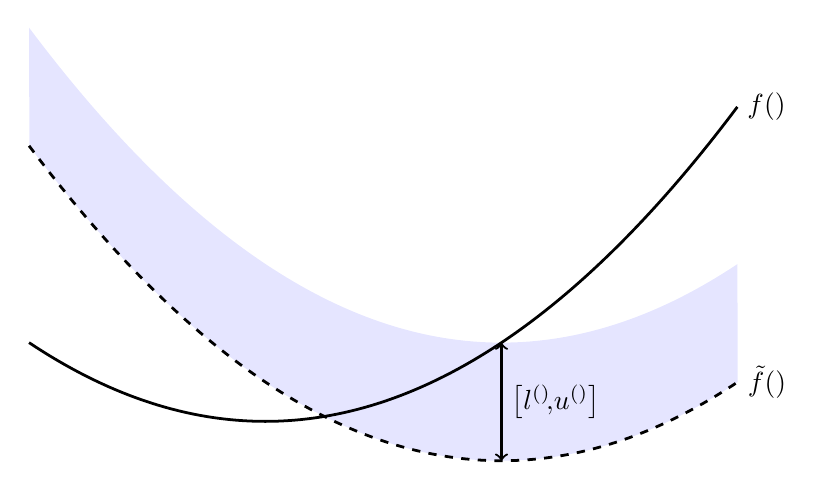
\begin{tikzpicture}[x=3cm, y=1cm]
  % Filled band around the quadratic curve with different boundary curves
\fill[blue!10] 
(-1, 5) -- plot[domain=-2:1, samples=100] ({\x+1}, {\x*\x + 1}) -- 
plot[domain=1:-2, samples=100] ({\x+1}, {\x*\x - 0.5}) -- cycle;
  \node[anchor=west] at (2, 4) {$f(\weights)$};
  \draw[line width=1, domain=-2:1, samples=100,dashed] plot  ({\x+1}, {\x*\x -0.5}) node[right] {$\tilde{f}(\weights)$};
   \draw[line width=1, domain=-1:2, samples=100] plot ({\x}, {\x*\x});
  \draw[<->, thick] (1, -0.5) -- (1, 1) node[midway, right] {$\big[ l^{(\weights)}\!,\!u^{(\weights)} \big]$};
\end{tikzpicture}
\caption{ML methods learn \gls{modelparams} $\weights$ by using some estimate $f(\weights)$ for 
	the ultimate performance criterion $\bar{f}(\weights)$. Using a \gls{probmodel}, one can use $f(\weights)$ to 
	construct confidence intervals $\big[ l^{(\weights)},  u^{(\weights)} \big]$ which contain $\bar{f}(\weights)$  
	with high probability. The best plausible performance measure for a specific choice $\weights$ of \gls{modelparams} 
	is $\tilde{f}(\weights) \defeq l^{(\weights)}$.} 
	\end{center}
		\end{figure}},first={optimism in face of uncertainty},text={optimism in face of uncertainty} 
}

\newglossaryentry{empgraph}
{name={federated learning (FL) network},
	description={A federated network\index{federated learning (FL) network} is an undirected weighted \gls{graph} whose 
		nodes represent data generators that aim to train a local (or personalized) \gls{model}. 
		Each node in a federated network represents some device, capable to collect a \gls{localdataset} 
		and, in turn, train a local \gls{model}. 
	    \Gls{fl} methods learn a local \gls{hypothesis} $\localhypothesis{\nodeidx}$, for 
	    each node $\nodeidx \in \nodes$, such that it incurs small \gls{loss} on the \gls{localdataset}s.},first={federated learning (FL) network},text={FL network} 
}

\newglossaryentry{norm}
{name={norm},
	description={A norm\index{norm} is a function that maps each element (vector) 
		of a linear vector space to a non-negative real number. This function must be 
		homogeneous, definite and satisfy the triangle inequality \cite{HornMatAnalysis}. },
	first={norm},text={norm} 
}

\newglossaryentry{explanation}
{name={explanation},
	description={One approach to make ML methods transparent, is to provide an 
		explanation\index{explanation} along with the \gls{prediction} delivered by an 
		ML method. Explanations can take on many different forms. An explanation 
		could be some natural text or some quantitative measure for the importance 
		of individual \gls{feature}s of a \gls{datapoint} \cite{Molnar2019}. We can also 
		use visual forms of explanations such as intensity plots for image classification \cite{GradCamPaper}.},
	first={explanation},text={explanation} 
}

\newglossaryentry{risk}
{name={risk},
	description={Consider\index{risk} a \gls{hypothesis} $\hypothesis$ used to predict the \gls{label} 
		$\truelabel$ of a \gls{datapoint} based on its \gls{feature}s $\featurevec$. We measure 
		the quality of a particular \gls{prediction} using a \gls{lossfunc} $\lossfunc{(\featurevec,\truelabel)}{\hypothesis}$. 
		If we interpret \gls{datapoint}s as the \gls{realization}s of \gls{iid} \gls{rv}s, 
		also the $\lossfunc{(\featurevec,\truelabel)}{\hypothesis}$ becomes the \gls{realization} 
		of a \gls{rv}. The \gls{iidasspt} allows to define the risk of a \gls{hypothesis} 
		as the expected \gls{loss} $\expect \big\{\lossfunc{(\featurevec,\truelabel)}{\hypothesis} \big\}$. 
		Note that the risk of $\hypothesis$ depends on both, the specific choice for the \gls{lossfunc} and the 
		\gls{probdist} of the \gls{datapoint}s.},
	first={risk},text={risk} 
}

\newglossaryentry{actfun}
{name={activation function},
	description={Each\index{activation function} artificial neuron within an \gls{ann} is 
		assigned an activation function $g(\cdot)$ that maps a weighted combination of 
		the neuron inputs $\feature_{1},\ldots,\feature_{\nrfeatures}$ to a single output 
		value $a = g\big(\weight_{1} \feature_{1}+\ldots+\weight_{\nrfeatures} \feature_{\nrfeatures} \big)$. 
		Note that each neuron is parameterized by the weights $\weight_{1},\ldots,\weight_{\nrfeatures}$.},
first={activation function},text={activation function} 
}




\newglossaryentry{transparency}
{name={transparency},
	description={Transparency\index{transparency} is a key requirement for 
		trustworthy AI \cite{HLEGTrustworhtyAI}. In the context of ML methods, 
		such as \gls{erm}-based methods, transparency is mainly used synonymously for \gls{explainability} \cite{gallese2023ai,JunXML2020}. 
		However, in the wide context of AI systems, transparency also includes providing information 
		about limitations and reliability of the AI system. As a point in case, \gls{logreg} provides a 
		quantitative measure of the reliability of a \gls{classification} in the form of the value $|\hypothesis(\featurevec)|$. 
		Transparency also includes the user interface, by requiring to clearly indicate when a user is 
		interaction with an AI system. Another component of transparency is the documentation 
		of the system’s purpose, design choices and intended use cases \cite{Shahriari2017,DatasheetData2021,10.1145/3287560.3287596}. },
	first={transparency},text={transparency} 
}


\newglossaryentry{sensattr}
{name={sensitive attribute},
	description={ML\index{sensitive attribute} revolves around learning a \gls{hypothesis} map that allows 
		to predict the \gls{label} of a \gls{datapoint} from its \gls{feature}s. In some 
		applications, we must ensure that the output delivered by an ML system does 
		not allow to infer sensitive attributes of a \gls{datapoint}. Which part 
		of a \gls{datapoint} is considered as a sensitive attribute is a design 
		choice that varies across different application domains.},
	first={sensitive attribute},text={sensitive attribute} 
}


\newglossaryentry{sbm}
{name={stochastic block model},
	description={The\index{stochastic block model} stochastic block model (SBM) is a 
		probabilistic generative model for an undirected graph $\graph = \big( \nodes, \edges \big)$ 
		with a given set of nodes $\nodes$ \cite{AbbeSBM2018}. In its most basic variant, 
		the SBM generates a graph by first randomly assigning each node $\nodeidx \in \nodes$ to 
		a cluster index $\clusteridx_{\nodeidx} \in \{1,\ldots,\nrcluster\}$. A pair of different nodes in the 
		graph is connected by an edge with probability $p_{\nodeidx,\nodeidx'}$ that depends 
		solely on the labels $\clusteridx_{\nodeidx}, \clusteridx_{\nodeidx'}$. 
		The presence of edges between different pairs of 
		nodes is statistically independent. },
	first={stochastic block model (SBM)},text={SBM} 
}

\newglossaryentry{deepnet}
{name={deep net},
	description={A\index{deep net} deep net is an \gls{ann} with a (relatively) large number of 
	hidden layers. Deep learning is an umbrella term for ML methods that use a deep net as 
	their model \cite{Goodfellow-et-al-2016}.},
	first={deep net},text={deep net} 
}

\newcommand{\gaussiancenter}{3}

\newglossaryentry{baseline}
{name={baseline},
    description={Consider\index{baseline} some ML method that delivers a learnt \gls{hypothesis} (or trained \gls{model}) 
    $\learnthypothesis \in \hypospace$. We evaluate the quality of a trained \gls{model} 
    by computing the average \gls{loss} on a \gls{testset}. But how do we know that the resulting 
    \gls{testset} performance is good (enough)? How can we determine if the trained \gls{model} performs 
    close to optimal and there is little point in investing more resources (for \gls{data} collection 
	or computation) to improve it? To this end, it is useful to have a reference (or baseline) level 
    against which we can compare the performance of the trained \gls{model}. 
    Such a reference value might be obtained from human performance, e.g., the misclassification
    rate of dermatologists who diagnose cancer from visual inspection of skin. Another 
    source for a baseline is an existing, but for some reason unsuitable, ML method. 
    For example, the existing ML method might be computationally too expensive for 
    the intended ML application. However, we might still use its \gls{testset} error 
    as a baseline. Another, somewhat more principled, approach to constructing a 
    baseline is via a \gls{probmodel}. For a wide range of \gls{probmodel}s $p(\featurevec,\truelabel)$ 
    we can precisely determine the minimum achievable \gls{risk} among \emph{any} \gls{hypothesis} (not even 
    required to belong to the \gls{hypospace} $\hypospace$) \cite{LC}. 
    This minimum achievable \gls{risk} (referred to as the \gls{bayesrisk}) is the \gls{risk} 
    of the \gls{bayesestimator} for the \gls{label} $\truelabel$ of a \gls{datapoint}, given
    its \gls{feature}s $\featurevec$. Note that, for a given choice of \gls{lossfunc}, the 
    \gls{bayesestimator} (if it exists) is completely determined by the \gls{probdist} $p(\featurevec,\truelabel)$ \cite[Chapter 4]{LC}. 
    However, there are two challenges to computing the \gls{bayesestimator} and \gls{bayesrisk}:
    i) the \gls{probdist} $p(\featurevec,\truelabel)$ is unknown and needs to be estimated 
    but (ii) even if we know $p(\featurevec,\truelabel)$ it might be computationally too expensive  
	to compute the \gls{bayesrisk} exactly. 
	\begin{figure}[h]
		\begin{center}
		\begin{tikzpicture}
			% Axes
			\draw[->] (-1,0) -- (7,0) node[right] {$\truelabel$}; % x-axis
			% Gaussian distribution centered at \gaussiancenter with variance 1
			\draw[thick,domain=-1:7,smooth,variable=\x] 
			  plot ({\x}, {2*exp(-0.5*((\x-\gaussiancenter)^2))});
			% Dashed line indicating the mean of the Gaussian
			\draw[dashed] (\gaussiancenter,0) -- (\gaussiancenter,2.5);
			\node[anchor=south] at ([yshift=-5pt] \gaussiancenter,2.5) {\small $\mu_{\truelabel|\featurevec}$};
			% Double arrow indicating the variance
			\draw[<->,thick] (\gaussiancenter-1,1) -- (\gaussiancenter+1,1.0);
			\node[anchor=west] at ([yshift=2pt] \gaussiancenter,1.2) {\small $\sigma_{\truelabel|\featurevec}$};
			% Posterior variance label
			%\node[anchor=south east] at (\gaussiancenter-0.5,1.8) {\small Posterior Variance};
			% x-axis marks with crosses
			  % x-axis marks with crosses
  			\foreach \x in {0.5} {
				\node[red] at (\x, 0) {\bf \large $\times$};
 			 }
  % h(x) label for the first cross
  			\node[anchor=north] at (0.5,-0.2) {\small $\learnthypothesis(\featurevec)$};
		  \end{tikzpicture}
		\end{center}
		\caption{If \gls{feature}s and \gls{label} of a \gls{datapoint} are drawn from a \gls{mvndist}, we 
		can achieve minimum \gls{risk} (under \gls{sqerrloss}) by using the \gls{bayesestimator} $\mu_{\truelabel|\featurevec}$ 
		to predict the \gls{label} $\truelabel$ of a \gls{datapoint} with \gls{feature}s $\featurevec$. The corresponding 
		minimum \gls{risk} is given by the posterior \gls{variance} $\sigma^{2}_{\truelabel|\featurevec}$. We can use 
		this quantity as a baseline for the average \gls{loss} of a trained \gls{model} $\learnthypothesis$. \label{fig_post_baseline}}
	\end{figure}
A widely used \gls{probmodel} is the \gls{mvndist} $\pair{\featurevec}{\truelabel} \sim \mathcal{N}({\bm \mu},{\bm \Sigma})$ 
for \gls{datapoint}s characterised by numeric \gls{feature}s and \gls{label}s.
Here, for the \gls{sqerrloss}, the \gls{bayesestimator} is given by the posterior 
mean $\mu_{\truelabel|\featurevec}$ of the \gls{label} $\truelabel$ given the 
\gls{feature}s $\featurevec$ \cite{LC,GrayProbBook}. The corresponding \gls{bayesrisk} 
is given by the posterior \gls{variance} 
$\sigma^{2}_{\truelabel|\featurevec}$ (see Figure \ref{fig_post_baseline}).},
    first={baseline},text={baseline}
}

\newglossaryentry{spectrogram}
{name={spectrogram},
	description={
		A\index{spectrogram} spectrogram represents the time-frequency distribution of the energy of a time signal $x(t)$.  
		Intuitively, it quantifies the amount of signal energy present within a specific time segment 
		$[t_{1},t_{2}] \subseteq \mathbb{R}$ and frequency interval $[f_{1},f_{2}]\subseteq \mathbb{R}$. 
		Formally, the spectrogram of a signal is defined as the squared magnitude of its 
		short-time Fourier transform (STFT) \cite{cohen1995time}.
        Figure \ref{fig:spectrogram} depicts a time signal along with its spectrogram. 
	\begin{figure}
		\centering
		\includegraphics[width=0.8\textwidth]{assets/spectrogram.png}
		\caption{Left: A time signal consisting of two modulated Gaussian pulses. Right: Intensity 
		plot of the spectrogram.
		\label{fig:spectrogram}}
	\end{figure}
        The intensity plot of its spectrogram can serve as an image of a signal. A 
		simple recipe for audio signal classification is to feed this \emph{signal image} 
		into \gls{deepnet}s originally developed for image classification and object detection \cite{Li:2022aa}. 
		It is worth noting that, beyond the spectrogram, several alternative representations exist 
		for the time-frequency distribution of signal energy \cite{TimeFrequencyAnalysisBoashash,MallatBook}. 
		}, 
	first={spectrogram},text={spectrogram} 
}

\newglossaryentry{graphclustering}
{name={graph clustering},
	description={Graph clustering\index{graph clustering} aims at 
		clustering \gls{datapoint}s that are represented as the nodes 
		of a \gls{graph} $\graph$. The edges of $\graph$ represent 
		pair-wise similarities between \gls{datapoint}s. Sometimes we
		can quantity the extend of these similarities by an edge weight \cite{Luxburg2007,FlowSpecClustering2021}. }, 
	first={graph clustering},text={graph clustering} 
}

\newglossaryentry{specclustering}
{name={spectral clustering},
	description={Spectral clustering\index{spectral clustering} is a particular instance of 
		\gls{graphclustering}, i.e., it clusters \gls{datapoint}s 
		represented as the nodes $\nodeidx=1,\ldots,\nrnodes$ of a \gls{graph} $\graph$. 
		Spectral clustering uses the \gls{eigenvector}s of the \gls{LapMat} $\LapMat{\graph}$ 
		to construct \gls{featurevec}s $\featurevec^{(\nodeidx)} \in \mathbb{R}^{\nrfeatures}$ 
		for each node (\gls{datapoint}) $\nodeidx=1,\ldots,\nrnodes$. We can feed these \gls{featurevec}s 
		into \gls{euclidspace}-based \gls{clustering} methods such as \gls{kmeans} 
		or \gls{softclustering} via \gls{gmm}. Roughly speaking, the \gls{featurevec}s of nodes 
		belonging to a well-connected subset (or \gls{cluster}) of nodes in $\graph$, are located 
		nearby in the \gls{euclidspace} $\mathbb{R}^{\nrfeatures}$ (see Figure \ref{fig_lap_mtx_specclustering}). 
		\begin{figure}
			\begin{center}
				\begin{minipage}{0.4\textwidth}
			\begin{tikzpicture}
				% Define the style for filled nodes
				\begin{scope}[every node/.style={circle, fill=black, inner sep=0pt, minimum size=0.3cm}]
					% Define nodes
					\node (1) at (0,0) {};
					\node (2) [below left=of 1, xshift=-0.2cm, yshift=-1cm] {};
					\node (3) [below right=of 1, xshift=0.2cm, yshift=-1cm] {};
					\node (4) [below=of 1, yshift=0.5cm] {}; % Isolated node
				\end{scope}
				% Draw edges
				\draw (1) -- (2);
				\draw (1) -- (3);
				% Add labels (separate from filled nodes)
				\node[above=0.2cm] at (1) {$\nodeidx=1$};
				\node[left=0.3cm] at (2) {$2$};
				\node[right=0.3cm] at (3) {$3$};
				\node[below=0.2cm] at (4) {$4$};
			\end{tikzpicture}
				\end{minipage} 
				\hspace*{5mm}
				\begin{minipage}{0.4\textwidth}
					\begin{equation} 
						\LapMat{\graph}\!=\!
						\begin{pmatrix} 
							2 & -1 & -1 & 0 \\ 
							-1 & 1 & 0 & 0 \\  
							-1 & 0 & 1 & 0 \\ 
							0 & 0 & 0 & 0 
						\end{pmatrix}\!=\!\mathbf{V} {\bm \Lambda} \mathbf{V}^{T}  
						\nonumber
					\end{equation} 
				\end{minipage}
				\vspace*{20mm}\\
				  \begin{minipage}{0.4\textwidth}
				\begin{tikzpicture}[scale=3]
%					% Axes
					\draw[->] (-0.2, 0) -- (1.2, 0) node[right] {$v^{(1)}_{\nodeidx}$};
					\draw[->] (0, -0.2) -- (0, 1.2) node[above] {$v^{(2)}_{\nodeidx}$};
%					
%					% Tailored tick marks and labels
%					\draw (0,0) node[below left] {$0$};
%					\draw (1/sqrt(3), 0) node[below] {$\frac{1}{\sqrt{3}}$} -- ++(0,0.05);
%					\draw (0, 1) node[left] {$1$} -- ++(0.05,0);
%					
%					 Data points
					\filldraw[blue] (0.577, 0) circle (0.03cm) node[above right] {$\nodeidx=1,2,3$};
					\filldraw[blue] (0.577, 0) circle (0.03cm); % Second point overlaps
					\filldraw[blue] (0.577, 0) circle (0.03cm); % Third point overlaps
					\filldraw[red] (0, 1) circle (0.03cm) node[above right] {$4$};
%					% Grid for reference
%					\draw[dashed, gray] (1/sqrt(3), 0) -- (1/sqrt(3), 1);
%					\draw[dashed, gray] (0, 1) -- (1, 1);
				\end{tikzpicture}
				\end{minipage} 
    		\begin{minipage}{0.4\textwidth}
										\begin{align}
											& \mathbf{V} = \big( \vv^{(1)},\vv^{(2)},\vv^{(3)},\vv^{(4)} \big) \nonumber \\
											&	\mathbf{v}^{(1)}\!=\!\frac{1}{\sqrt{3}} \begin{pmatrix} 1 \\ 1 \\ 1 \\ 0 \end{pmatrix}, \,
												\mathbf{v}^{(2)}\!=\!\begin{pmatrix} 0 \\ 0 \\ 0 \\ 1 \end{pmatrix} \nonumber 
												\end{align}
				\end{minipage} 
				\caption{\label{fig_lap_mtx_specclustering} {\bf Top.} Left: An undirected \gls{graph} 
					$\graph$ with four nodes $\nodeidx=1,2,3,4$, each representing a \gls{datapoint}. Right: Laplacian matrix 
					$\LapMat{\graph}  \in \mathbb{R}^{4 \times 4}$ and its \gls{evd}. 
					{\bf Bottom.} Left: \Gls{scatterplot} of \gls{datapoint}s using the \gls{featurevec}s 
					$\featurevec^{(\nodeidx)} = \big( v^{(1)}_{\nodeidx},v^{(2)}_{\nodeidx} \big)^{T}$. 
					Right: Two \gls{eigenvector}s $\vv^{(1)},\vv^{(2)} \in \mathbb{R}^{\nrfeatures}$ 
					of the \gls{LapMat} $\LapMat{\graph}$ corresponding to the \gls{eigenvalue} $\lambda=0$. 
					} 
			\end{center}
		\end{figure}
	\newpage}, 
	first={spectral clustering},text={spectral clustering} 
}

\newglossaryentry{flowbasedclustering}
{name={flow-based clustering},
	description={Flow-basted clustering\index{flow-based clustering} groups the nodes 
		of an undirected graph by applying \gls{kmeans} clustering to node-wise feature 
		vectors. These \gls{feature} vectors are built from networks flows between 
		carefully selected source and destination nodes \cite{FlowSpecClustering2021}. }, 
	first={flow-based clustering},text={flow-based clustering} 
}



\newglossaryentry{esterr}
{name={estimation error},
	description={Consider\index{estimation error} \gls{datapoint}s, each with \gls{featurevec} $\featurevec$ and \gls{label} 
		$\truelabel$. In some applications we can model the relation between the \gls{featurevec} and the \gls{label}
		of a \gls{datapoint} as $\truelabel = \bar{\hypothesis}(\featurevec) + \varepsilon$. Here, we 
		used some true underlying \gls{hypothesis} $\bar{\hypothesis}$ and a noise term $\varepsilon$ 
		which summarized any modelling or labelling errors. The estimation error incurred by an ML 
		method that learns a \gls{hypothesis} $\widehat{\hypothesis}$, e.g., using \gls{erm}, is defined as 
		$\widehat{\hypothesis}(\featurevec) - \bar{\hypothesis}(\featurevec)$, for some \gls{featurevec}. 
		For a parametric \gls{hypospace}, consisting of \gls{hypothesis} maps that are determined by 
		\gls{modelparams} $\weights$, we can define the estimation error as $\Delta \weights = \widehat{\weights} - \overline{\weights}$ \cite{kay,hastie01statisticallearning}.},
	first={estimation error},text={estimation error} 
}


\newglossaryentry{dob}
{name={degree of belonging},
	description={A\index{degree of belonging} number that indicates the extent to which a \gls{datapoint} 
		belongs to a \gls{cluster} \cite[Ch. 8]{MLBasics}. The degree of belonging can be 
		interpreted as a soft \gls{cluster} assignment. \Gls{softclustering} methods can 
		encode the degree of belonging by a real number in the interval $[0,1]$. 
		\Gls{hardclustering} is obtained as the extreme case when the degree of belonging 
		only takes on values $0$ or $1$.}, first={degree of belonging},text={degree of belonging} 
}

\newglossaryentry{msee}
{name={mean squared estimation error},
	description={Consider\index{mean squared estimation error} an ML method that 
		learns \gls{modelparams} $\widehat{\weights}$ based on some \gls{dataset} $\dataset$. 
		If we interpret the \gls{datapoint}s in $\dataset$ as \gls{iid} \gls{realization}s of a \gls{rv} $\datapoint$, 
		we define the \gls{esterr} $\Delta \weights \defeq \widehat{\weight} - \overline{\weights}$. 
		Here, $\overline{\weights}$ denotes the true \gls{modelparams} of the \gls{probdist} 
		of $\datapoint$.The mean squared estimation error is 
		defined as the \gls{expectation} $\expect \big\{ \big\| \Delta \weights \big\|^{2} \big\}$ of the 
		squared Euclidean norm of the \gls{esterr} \cite{LC,kay}.},
	first={mean squared estimation error (MSEE)},text={MSEE} 
}

\newglossaryentry{gtvmin}
{name={GTV minimization},
	description={GTV minimization\index{total variation minimization} is an instance of \gls{rerm} 
		using the \gls{gtv} of local \gls{modelparams} as a \gls{regularizer} \cite{ClusteredFLTVMinTSP}.},
	first={GTV minimization (GTVMin)},text={GTVMin} 
}

\newglossaryentry{regression}
{name={regression},
	description={Regression\index{regression} problems revolve around the problem of 
		predicting a numeric \gls{label} solely from the \gls{feature}s of a \gls{datapoint} \cite[Ch. 2]{MLBasics}.},
	first={regression},text={regression} 
}

\newglossaryentry{acc}
{name={accuracy},
	description={Consider\index{accuracy} \gls{datapoint}s characterized by \gls{feature}s $\featurevec \in \featurespace$ and 
		a categorical label $\truelabel$ which takes on values from a finite \gls{labelspace} $\labelspace$. The 
		accuracy of a \gls{hypothesis} $\hypothesis: \featurespace \rightarrow \labelspace$, when applied 
		to the \gls{datapoint}s in a \gls{dataset} $\dataset = \big\{ \big(\featurevec^{(1)}, \truelabel^{(1)} \big), \ldots, \big(\featurevec^{(\samplesize)},\truelabel^{(\samplesize)}\big) \big\}$ 
		is then defined as $1 - (1/\samplesize)\sum_{\sampleidx=1}^{\samplesize} \lossfunc{\big(\featurevec^{(\sampleidx)},\truelabel^{(\sampleidx)}\big)}{\hypothesis}$ using the \gls{zerooneloss}.},
	first={accuracy},text={accuracy} 
}



\newglossaryentry{expert}
{name={expert},
	description={ML\index{expert} aims to learn a \gls{hypothesis} $\hypothesis$ that accurately predicts the \gls{label} 
		of a \gls{datapoint} based on its \gls{feature}s. We measure the prediction error using 
		some \gls{lossfunc}. Ideally, we want to find a \gls{hypothesis} that incurs minimal \gls{loss} 
		on any \gls{datapoint}. We can make this informal goal precise via the \gls{iidasspt} 
		and using the \gls{bayesrisk} as the \gls{baseline} for the (average) \gls{loss} of a \gls{hypothesis}. 
		An alternative approach to obtain a \gls{baseline} is to use the \gls{hypothesis} $\hypothesis'$ learnt 
		by an existing ML method. We refer to this \gls{hypothesis} $\hypothesis'$ as an expert \cite{PredictionLearningGames}. Regret minimization methods learn a \gls{hypothesis}
		that incurs a \gls{loss} comparable to the best expert \cite{PredictionLearningGames,HazanOCO}.},
	first={expert},text={expert} 
}

\newglossaryentry{nfl}
{name={networked federated learning},
	description={Networked\index{networked federated learning} federated learning refers 
		to methods that learn personalized models in a distributed fashion from \gls{localdataset}s 
		that are related by an intrinsic network structure.},
 first={networked federated learning (NFL)},text={NFL} 
}




\newglossaryentry{regret}
{name={regret},
	description={The regret\index{regret} of a \gls{hypothesis} $\hypothesis$ relative to 
		another \gls{hypothesis} $\hypothesis'$, which serves as a \gls{baseline}, 
		is the difference between the \gls{loss} incurred by $\hypothesis$ and the \gls{loss} 
		incurred by $\hypothesis'$ \cite{PredictionLearningGames}. 
		The \gls{baseline} \gls{hypothesis} $\hypothesis'$ is also referred to as an \gls{expert}.},
	first={regret},text={regret} 
}

\newglossaryentry{strcvx}
{name={strongly convex},
	description={A\index{strongly convex} continuously \gls{differentiable} real-valued 
		function $f(\featurevec)$ is strongly convex with coefficient $\sigma$ if $f(\vy) \geq f(\vx) + \nabla f(\vx)^{T} (\vy - \vx) + (\sigma/2) \normgeneric{\vy - \vx}{2}^{2}$ \cite{nesterov04},\cite[Sec. B.1.1.]{CvxAlgBertsekas}.},
	first={strongly convex},text={strongly convex} 
}

\newglossaryentry{differentiable}
{name={differentiable},
	description={A\index{differentiable} function real-valued function $f: \mathbb{R}^{\featuredim} \rightarrow \mathbb{R}$ 
		is differentiable if it can, at any point, be approximated locally by a linear 
		function. The local linear approximation at the point $\mathbf{x}$ is determined 
		by the \gls{gradient} $\nabla f ( \mathbf{x})$ \cite{RudinBookPrinciplesMatheAnalysis}.},
	first={differentiable},text={differentiable} 
}

\newglossaryentry{gradient}
{name={gradient},
	description={For\index{gradient} a real-valued function $f: \mathbb{R}^{\featuredim} \rightarrow \mathbb{R}: \weights \mapsto f(\weights)$, 
	a vector $\vg$ such that $\lim_{\weights \rightarrow \weights'} \frac{f(\weights) - \big(f(\weights')+ \vg^{T} (\weights- \weights') \big) }{\| \weights-\weights'\|}=0$ 
	is referred to as the gradient of $f$ at $\weights'$. If such a vector exists it is 
	denoted $\nabla f(\weights')$ or $\nabla f(\weights)\big|_{\weights'}$ \cite{RudinBookPrinciplesMatheAnalysis}.},
	first={gradient},text={gradient} 
}

\newglossaryentry{subgradient}
{name={subgradient},
description={For\index{subgradient} a real-valued function $f: \mathbb{R}^{\featuredim} \rightarrow \mathbb{R}: \weights \mapsto f(\weights)$, 
		a vector $\va$ such that $f(\weights) \geq  f(\weights') +\big(\weights-\weights' \big)^{T} \va$ is 
		referred to as a subgradient of $f$ at $\weights'$ \cite{BertCvxAnalOpt,BertsekasNonLinProgr}.},
	first={subgradient},text={subgradient} 
}

\newglossaryentry{fedavg}
{name={federated averaging (FedAvg)},
	description={An\index{federated averaging (FedAvg)} iterative \gls{fl} 
		algorithm that alternates between the separate training of \gls{localmodel}s, followed by 
		combining the updated local \gls{modelparams}. The training of \gls{localmodel}s 
		is implemented via several \gls{stochGD} steps \cite{pmlr-v54-mcmahan17a}.}, 
		first = {federated averaging (FedAvg)}, text={FedAvg} 
}

\newglossaryentry{fedprox}
{name={FedProx},
	description={An\index{FedProx} iterative \gls{fl} 
		algorithm that alternates between the separate training of \gls{localmodel}s, followed by 
		combining the updated local \gls{modelparams}. In contrast to \gls{fedavg}, which uses 
		\gls{stochGD} to train \gls{localmodel}s, FedProx uses a \gls{proxop} for the training \cite{FedProx2020}.}, 
	first = {FedProx}, text={FedProx} 
}

\newglossaryentry{relu}
{name={rectified linear unit (ReLU)},
	description={The\index{rectified linear unit (ReLU)} rectified linear unit (ReLU) is 
		a popular choice for the \gls{actfun} of a neuron within an \gls{ann}. It is defined 
		as $g(z) = \max\{0,z\}$ with $z$ being the weighted input of the artificial neuron.}, first = {rectified linear unit (ReLU)}, text={ReLU} 
}

\newglossaryentry{hypothesis}
{name={hypothesis},
	description={A\index{hypothesis} map (or function) $\hypothesis: \featurespace \rightarrow \labelspace$ from the 
		\gls{featurespace} $\featurespace$ to the \gls{labelspace} $\labelspace$. 
		Given a \gls{datapoint} with \gls{feature}s $\featurevec$, we use a hypothesis map $\hypothesis$
		to estimate (or approximate) the \gls{label} $\truelabel$ using the \gls{prediction}  
		$\hat{\truelabel} = \hypothesis(\featurevec)$. ML is all about learning (or finding) a 
		hypothesis map $\hypothesis$ such that $\truelabel \approx \hypothesis(\featurevec)$ 
		for any \gls{datapoint} (having \gls{feature}s $\featurevec$ and \gls{label} $\truelabel$).},
	first={hypothesis},text={hypothesis}  
}



\newglossaryentry{vcdim}
{name={Vapnik?Chervonenkis (VC) dimension},
	description={The\index{VC dimension} VC dimension of an infinite \gls{hypospace} is a widely-used measure 
		for its size. We refer to \cite{ShalevMLBook} for a precise definition of VC dimension 
		as well as a discussion of its basic properties and use in ML.},
	first={Vapnik?Chervonenkis (VC) dimension},text={VC dimension}  
}

\newglossaryentry{effdim}
{name={effective dimension},
	description={The\index{effective dimension} effective dimension $\effdim{\hypospace}$ of 
		an infinite \gls{hypospace} $\hypospace$ is a measure of its size. Loosely speaking, the 
		effective dimension is equal to the effective number of independent tunable parameters 
		of the model. These parameters might be the coefficients used in a linear map or the 
		weights and bias terms of an \gls{ann}.},
	first={effective dimension},text={effective dimension}  
}

\newglossaryentry{labelspace}
{name={label space},
	description={Consider\index{label space} an ML application that involves \gls{datapoint}s characterized by features 
		and labels. The \gls{label} space is constituted by all potential values that the \gls{label} 
		of a \gls{datapoint} can take on. Regression methods, aiming at predicting numeric \gls{label}s, often
		 use the \gls{label} space $\labelspace = \mathbb{R}$. Binary \gls{classification} methods use a label space 
 		that consists of two different elements, e.g., $\labelspace =\{-1,1\}$, $\labelspace=\{0,1\}$ 
		or $\labelspace = \{ \mbox{``cat image''}, \mbox{``no cat image''} \}$  }, first={label space},text={label space}  
}

\newglossaryentry{prediction}
{name={prediction},
	description={A\index{prediction} prediction is an estimate or approximation for some 
		quantity of interest. ML revolves around learning or finding a \gls{hypothesis} map $\hypothesis$ 
		that reads in the \gls{feature}s $\featurevec$ of a \gls{datapoint} and delivers a \gls{prediction} 
		$\widehat{\truelabel} \defeq \hypothesis(\featurevec)$ for its \gls{label} $\truelabel$. },
	first={prediction},text={prediction}  
}


\newglossaryentry{histogram}
{name={histogram},
	description={Consider\index{histogram} a \gls{dataset} $\dataset$ that consists of $\samplesize$ \gls{datapoint}s 
		$\datapoint^{(1)},\ldots,\datapoint^{(\samplesize)}$, each of them belonging to some 
		cell $[-U,U] \times \ldots \times [-U,U] \subseteq \mathbb{R}^{\featuredim}$ with side 
		length $U$. We partition this cell evenly into smaller elementary cells with side 
		length $\Delta$. The histogram of $\dataset$ assigns each elementary cell to 
		the corresponding fraction of \gls{datapoint}s in $\dataset$ that fall into this 
		elementary cell. 
	},
	first={histogram},text={histogram}  
}

\newglossaryentry{bootstrap}
{name={bootstrap},
	description={For\index{bootstrap}  the analysis of ML methods it is often useful to interpret 
		a given set of \gls{datapoint}s $\dataset = \big\{ \datapoint^{(1)},\ldots,\datapoint^{(\samplesize)}\big\}$ 
		as \gls{realization}s of \gls{iid} \gls{rv}s with a common \gls{probdist} $p(\datapoint)$. In general, we 
		do not know $p(\datapoint)$ exactly, but we need to estimate it. The bootstrap uses the 
		histogram of $\dataset$ as an estimator for the underlying \gls{probdist} $p(\datapoint)$. 
	},
	first={bootstrap},text={bootstrap}  
}

\newglossaryentry{featurespace}
{name={feature space},
	description={
		The\index{feature space} \gls{feature} space of a given ML application or method is 
		constituted by all potential values that the \gls{feature} vector of a \gls{datapoint} can 
		take on. A widely used choice for the feature space is the \gls{euclidspace} $\mathbb{R}^{\featuredim}$ 
		with dimension $\featurelen$ being the number of individual \gls{feature}s of a \gls{datapoint}.},
	first={feature space},text={feature space}  
}


\newglossaryentry{missingdata}
{name={missing data},
	description={Consider\index{missing data} a \gls{dataset} constituted by \gls{datapoint}s collected via 
		some physical device. Due to imperfections and failures, some of the \gls{feature} 
		or \gls{label} values of \gls{datapoint}s might be corrupted or simply \emph{missing}. 
		Data imputation aims at estimating these missing values \cite{Abayomi2008DiagnosticsFM}. 
		We can interpret data imputation as an ML problem where the \gls{label} of a \gls{datapoint} is 
		the value of the corrupted \gls{feature}. },
	first={missing data},text={missing data}  
}


\newglossaryentry{psd}
{name={positive semi-definite},
	description=
	{A\index{positive semi-definite} (real-valued) symmetric matrix $\mQ = \mQ^{T} \in \mathbb{R}^{\featuredim \times \featuredim}$ 
	 is referred to as positive semi-definite if $\featurevec^{T} \mQ \featurevec \geq 0$ for every vector $\featurevec \in \mathbb{R}^{\featuredim}$. 
	 The property of being psd can be extended from matrices to (real-valued) 
	 symmetric \gls{kernel} maps $\kernel: \featurespace \times \featurespace \rightarrow \mathbb{R}$ 
	 (with $\kernel(\featurevec,\featurevec') = \kernel(\featurevec',\featurevec)$)
	 as follows: for any finite set of \gls{feature} vectors $\featurevec^{(1)},\dots,\featurevec^{(\samplesize)}$, 
	 the resulting matrix $\mQ \in \mathbb{R}^{\samplesize \times \samplesize}$ with 
	entries $Q_{\sampleidx,\sampleidx'} = \kernelmap{\featurevec^{(\sampleidx)}}{\featurevec^{(\sampleidx')}}$ 
	is psd \cite{LearningKernelsBook}.},
	first={positive semi-definite (psd)},text={psd}  
}

\newglossaryentry{feature}
{name={feature},
	description={A\index{feature} feature of a \gls{datapoint} is one of its properties that can be 
		measured or computed easily without the need for human supervision. For example, if a \gls{datapoint} 
		is a digital image (e.g, stored as a \texttt{.jpeg} file), then we could use the red-green-blue intensities 
		of its pixels as features. Domain-specific synonyms for the term feature are \emph{covariate}, \emph{explanatory variable}, 
		\emph{independent variable}, \emph{input (variable)}, \emph{predictor (variable)} or \emph{regressor} \cite{Gujarati2021,Dodge2003,Everitt2022}. 
		}, first={feature},text={feature}  
}

\newglossaryentry{featurevec}
{name={feature vector},
	description={A\index{feature vector} vector $\vx = \big(x_{1},\ldots,x_{\nrfeatures}\big)^{T}$ 
	whose entries are individual \gls{feature}s $x_{1},\ldots,x_{\nrfeatures}$. Many ML methods 
	use feature vectors that belong to some finite-dimensional \gls{euclidspace} $\mathbb{R}^{\nrfeatures}$. 
	For some ML methods, it can be more convenient to work with feature 
	vectors that belong to an infinite-dimensional vector space (see, e.g., \gls{kernelmethod}). 
		}, first={feature vector},text={feature vector}  
}


\newglossaryentry{label}
{name={label},
	description={A\index{label} higher-level fact or quantity of interest associated with a \gls{datapoint}. 
		For example, if the \gls{datapoint} is an image, the label could indicate whether the 
		image contains a cat or not. Synonyms for label, commonly used in specific domains, 
		include \emph{response variable}, \emph{output variable}, and \emph{target} \cite{Gujarati2021,Dodge2003,Everitt2022}.
 },
	first={label},text={label}  
}


\newglossaryentry{data}
{name={data},
	 description={See\index{data} \gls{dataset}.},
	text={data}
}

\newglossaryentry{dataset}
{name={dataset},
	description={A\index{dataset} dataset consists of one or more \gls{datapoint}s and is 
		the main component of most ML methods. These methods use datasets to train and 
		validate ML \gls{model}s. Different mathematical models and formal languages are 
		used to describe datasets and the ML methods that operate on them \cite{silberschatz2019database,abiteboul1995foundations,hoberman2009data,ramakrishnan2002database}. 
		One of the most widely adopted data model is the relational model, 
		which organizes data as a table (or relation) \cite{silberschatz2019database}.
		A table consists of rows and columns:
		\begin{itemize} 
		\item Each row of the table represents a single \gls{datapoint}.
		\item Each column of the table corresponds to a specific attribute of the \gls{datapoint}, including its \gls{feature}s and \gls{label}s.
		\end{itemize}
		For example, Table \ref{tab:temperature} shows a dataset containing weather observations. 
		In the relational model, the order of rows is irrelevant, and each attribute (column) must be 
		precisely defined with a domain, which specifies the set of possible values. These attribute 
		domains correspond to the \gls{featurespace} and \gls{labelspace} of the \gls{datapoint}s.
		\begin{table}[ht]
	\centering
	\begin{tabular}{|l|c|c|c|c|c|}
		\hline
		\textbf{FMI Station} & \textbf{Year} & \textbf{Month} & \textbf{Day} & \textbf{Time} & \textbf{Temp. [°C]} \\ 
		\hline
		Kustavi Isokari & 2023 & 4 & 1 & 00:00 & -0.2 \\ \hline
		Kustavi Isokari & 2023 & 4 & 2 & 00:00 & -0.1 \\ \hline
		Kustavi Isokari & 2023 & 4 & 3 & 00:00 & -1.0 \\ \hline
		Kustavi Isokari & 2023 & 4 & 4 & 00:00 & -0.4 \\ \hline
		Kustavi Isokari & 2023 & 4 & 5 & 00:00 & 0.9 \\ \hline
	\end{tabular}
	\caption{Temperature observations at FMI station Kustavi Isokari.}
	\label{tab:temperature}
\end{table}
 While the relational model is useful for the study of many ML applications, it may be 
 insufficient regarding the requirements for trustworthy AI. Modern 
 approaches like \emph{datasheets for datasets} provide more comprehensive 
 documentation, including details about the dataset’s collection process, intended 
 use, and other contextual information \cite{DatasheetData2021}.},first={dataset},text={dataset}  
}

\newglossaryentry{predictor}
{name={predictor},
	description={A\index{predictor} predictor is a real-valued \gls{hypothesis} map. 
		Given a \gls{datapoint} with \gls{feature}s $\featurevec$, the value 
		$\hypothesis(\featurevec) \in \mathbb{R}$ is used as a \gls{prediction} for the true 
		numeric label $\truelabel \in \mathbb{R}$ of the \gls{datapoint}. },first={predictor},text={predictor}  
}

\newglossaryentry{labeled datapoint}
{name={labeled datapoint},
 description={A\index{labeled data} \gls{datapoint} whose \gls{label} is known or has been determined 
 	by some means which might involve human experts.},
 first={labeled datapoint},text={labeled datapoint}  
}

\newglossaryentry{rv}
{name={random variable (RV)},
 description={A\index{random variable (RV)} random\index{probability space} 
 		variable is a mapping from a probability space $\mathcal{P}$ to a value space \cite{BillingsleyProbMeasure}. 
 	The probability space, whose elements are elementary events, is equipped with a probability 
 	 measure that assigns a probability to subsets of $\mathcal{P}$. A binary random variable maps elementary events 
 	to a set containing two different values, e.g., $\{-1,1\}$ or $\{ \mbox{cat}, \mbox{no cat} \}$. 
 	A real-valued random variable maps elementary events to real numbers $\mathbb{R}$. 
 	A vector-valued random variable maps elementary events to the \gls{euclidspace} $\mathbb{R}^{\featuredim}$. 
 	Probability theory uses the concept of measurable spaces to rigorously define and study the properties of (large) 
 	collections of random variables \cite{GrayProbBook,BillingsleyProbMeasure}.}, first={RV},text={RV}  }
 
	
\newglossaryentry{realization}
{name={realization},
	description={Consider\index{realization} a \gls{rv} $x$ which maps each element 
	(outcome or elementary event) $\omega \in \mathcal{P}$ of a probability space $\mathcal{P}$ 
	to an element $a$ of a measurable space $\mathcal{N}$ \cite{BillingsleyProbMeasure,RudinBookPrinciplesMatheAnalysis,HalmosMeasure}. 
	A realization of $x$ is any element $a' \in \mathcal{N}$ such that there is 
	an element $\omega' \in \mathcal{P}$ with $x(\omega') = a'$.}, first={realization},text={realization}  }

\newglossaryentry{trainset}
{name={training set},
description={A\index{training set} \gls{dataset} $\dataset$, constituted by some \gls{datapoint}s used in \gls{erm} 
	to learn a \gls{hypothesis} $\learnthypothesis$. The average \gls{loss} of $\learnthypothesis$ on the 
	training set is referred to as the \gls{trainerr}. The comparison of the \gls{trainerr} with the 
	\gls{valerr} of $\learnthypothesis$ allows to diagnose the ML method and informs how to improve 
	them (e.g., using a different \gls{hypospace} or collecting more \gls{datapoint}s) \cite[Sec. 6.6.]{MLBasics}.},first={training set},text={training set}  
}

\newglossaryentry{netmodel}
{name={networked model},
  description={A\index{networked model} networked model over an \gls{empgraph} $\graph = \pair{\nodes}{\edges}$ assigns 
   a \gls{localmodel} (\gls{hypospace}) to each node $\nodeidx \in \nodes$ of the \gls{empgraph} $\graph$.}, 
   first={networked model},text={networked model}  
}

\newglossaryentry{batch}
{
	name={batch},
	description={In\index{batch} the context of \gls{stochGD}, a batch refers to a randomly 
	chosen subset of the overall \gls{trainset}. We use the \gls{datapoint}s in this subset 
	to estimate the \gls{gradient} of \gls{trainerr} and, in turn, to update the \gls{modelparams}.}, 
	first={batch},text={batch}  
}

\newglossaryentry{netdata}
{
	name={networked data},
	description={Networked\index{networked data} data consists of \gls{localdataset}s 
	that are related by some notion of pair-wise similarity. We can represent networked 
	data using a \gls{graph} whose nodes carry \gls{localdataset}s and edges encode 
	pairwise similarities. One example of \gls{netdata} arises in \gls{fl} applications 
	where \gls{localdataset}s are generated by spatially distributed devices.}, 
	first={networked data},text={networked data}  
}

\newglossaryentry{trainerr}
{
	name={training error},
	description={The\index{training error} average \gls{loss} of a \gls{hypothesis} when 
		predicting the \gls{label}s of the \gls{datapoint}s in a \gls{trainset}. 
		We sometimes refer by training error also to minimal average \gls{loss} 
		which is achieved by a solution of \gls{erm}.},first={training error},text={training error}  
}

\newglossaryentry{datapoint}
{name={data point},
description={A\index{data point} \gls{datapoint} is any object that conveys information \cite{coverthomas}. Data points might be 
		students, radio signals, trees, forests, images, \gls{rv}s, real numbers or proteins. We characterize data points 
		using two types of properties. One type of property is referred to as a \gls{feature}. \Gls{feature}s are properties of a 
		\gls{datapoint} that can be measured or computed in an automated fashion. 
		A different kind of property is referred to as \gls{label}s. The \gls{label} of 
		a \gls{datapoint} represents some higher-level fact (or quantity of interest). In 
		contrast to \gls{feature}s, determining the \gls{label} of a \gls{datapoint} typically 
		requires human experts (domain experts). Roughly speaking, ML aims to predict 
		the \gls{label} of a \gls{datapoint} based solely on its \gls{feature}s. 
		}, first={data point},text={data point}  
}


\newglossaryentry{valerr}
{name={validation error},
 description={Consider\index{validation error} a \gls{hypothesis} $\learnthypothesis$ which is 
 	obtained by some ML method, e.g., using \gls{erm} on a \gls{trainset}. The average \gls{loss} 
 	of $\learnthypothesis$ on a \gls{valset}, which is different from the \gls{trainset}, is referred 
 	to as the validation error.},first={validation error},text={validation error}  
}

\newglossaryentry{validation} 
{name={validation},
	description={Consider\index{validation} a \gls{hypothesis} $\learnthypothesis$ that has been 
		learnt via some ML method, e.g., by solving \gls{erm} on a \gls{trainset} $\dataset$. 
		Validation refers to the practice of evaluating the \gls{loss} incurred by 
		\gls{hypothesis} $\learnthypothesis$ on a \gls{valset} that consists of 
		\gls{datapoint}s that are not contained in the \gls{trainset} $\dataset$. },first={validation},text={validation}  
}

\newglossaryentry{quadfunc}
{name={quadratic function},
	description={A\index{quadratic function} function $f: \mathbb{R}^{\nrfeatures} \rightarrow \mathbb{R}$ of the form 
	$$f(\weights) =  \weights^{T} \mathbf{Q} \mathbf{w} + \mathbf{q}^{T} \weights+a,$$ with 
	some matrix $\mQ \in \mathbb{R}^{\nrfeatures \times \nrfeatures}$, vector $\vq \in \mathbb{R}^{\nrfeatures}$ 
	and scalar $a \in \mathbb{R}$.  },first={quadratic function},text={quadratic function}  
}

\newglossaryentry{valset}
{name={validation set},
  description={A\index{validation set} set of \gls{datapoint}s used to estimate 
  	the \gls{risk} of a \gls{hypothesis} $\learnthypothesis$ that has been learnt by some 
  	ML method (e.g., solving \gls{erm}). The average \gls{loss} of $\learnthypothesis$ 
  	on the validation set is referred to as the validation error and can be used to diagnose a 
  	ML method (see \cite[Sec. 6.6.]{MLBasics}). The comparison between \gls{trainerr} 
  	and \gls{valerr} can inform directions for improvements of the ML method (such as 
  	using a different \gls{hypospace}).},first={validation set},text={validation set}  
}

\newglossaryentry{testset}
{name={test set},
	description={A\index{test set} set of \gls{datapoint}s that have neither 
		been used to train a \gls{model}, e.g., via \gls{erm}, nor in a \gls{valset} 
		to choose between different \gls{model}s.},first={test set},text={test set}  
}


\newglossaryentry{modelsel}
{name={model selection},
	description={In\index{model selection} ML, model selection refers to the 
		process of choosing between different candidate \gls{model}s. In its most 
		basic form, \gls{model} selection amounts to (i) training each candidate \gls{model}, 
		(ii) computing the \gls{valerr} for each trained \gls{model}, (iii) choosing the \gls{model} 
		with smallest \gls{valerr} \cite[Ch. 6]{MLBasics}. },first={model selection},text={model selection}  
}





\newglossaryentry{linclass}{name={linear classifier}, description={
	    Consider\index{linear classifier} \gls{datapoint}s characterized by numeric \gls{feature}s $\featurevec \in \mathbb{R}^{\nrfeatures}$ 
	    and a \gls{label} $\truelabel \in \labelspace$ from some finite \gls{labelspace} $\labelspace$. 
		A linear \gls{classifier} is characterized by having \gls{decisionregion}s that are 
		separated by hyperplanes in $\mathbb{R}^{\featuredim}$ \cite[Ch. 2]{MLBasics}.},first={linear classifier},text={linear classifier} }

\newglossaryentry{erm}{name={empirical risk minimization}, description={Empirical risk 
		minimization\index{empirical risk minimization} is the optimization problem of finding 
		a \gls{hypothesis} (out of a \gls{model}) with minimum average \gls{loss} (or \gls{emprisk}) on a given \gls{dataset} 
		$\dataset$ (the \gls{trainset}). Many ML methods are obtained from 
		\gls{emprisk} via specific design choices for the \gls{dataset}, \gls{model} and \gls{loss} \cite[Ch. 3]{MLBasics}.},
	first={empirical risk minimization (ERM)},text={ERM} }

\newglossaryentry{multilabelclass}{name={multi-label classification}, description={Multi-label 
		classification\index{multi-label classification} problems and methods use \gls{datapoint}s 
		that are characterized by several \gls{label}s. As an example, consider a \gls{datapoint} 
		representing a picture with one binary \gls{label} indicating the presence of a human 
		in this picture and another \gls{label} indicating the presence of a car.},
	    first={multi-label classification},text={multi-label classification} }


\newglossaryentry{ssl}{name={semi-supervised learning}, description={Semi-supervised\index{semi-supervised learning} 
		learning methods use unlabeled \gls{datapoint}s to support the learning of a \gls{hypothesis} 
		from labeled \gls{datapoint}s \cite{SemiSupervisedBook}. This approach is particularly useful 
		for ML applications that offer a large amount of unlabeled \gls{datapoint}s, but only a limited 
		number of  labeled \gls{datapoint}s.}, 
		first={semi-supervised learning (SSL)},text={SSL} }
	
	
\newglossaryentry{objfunc}{name={objective function}, description={An\index{objective function} 
		objective function is a map that assigns each value of an optimization variable, such 
		as the \gls{modelparams} $\weights$ of a \gls{hypothesis} $\hypothesis^{(\weights)}$, to 
		an objective value $f(\weights)$. The objective value $f(\weights)$ could be the 
		\gls{risk} or the \gls{emprisk} of a \gls{hypothesis} $\hypothesis^{(\weights)}$.},first={objective function},text={objective function} }
	
\newglossaryentry{regularizer}{name={regularizer}, description={A regularizer\index{regularizer} 
		assigns each \gls{hypothesis} $\hypothesis$ from a \gls{hypospace} $\hypospace$ a quantitative 
		measure $\regularizer{\hypothesis}$ for how much its prediction error on a \gls{trainset} might 
		differ from its prediction errors on \gls{datapoint}s outside the \gls{trainset}. \Gls{ridgeregression} 
		uses the regularizer $\regularizer{\hypothesis} \defeq \normgeneric{\weights}{2}^{2}$ for linear \gls{hypothesis} maps $\hypothesis^{(\weights)}(\featurevec) \defeq \weights^{T} \featurevec$ \cite[Ch. 3]{MLBasics}. 
		\Gls{lasso} uses the regularizer $\regularizer{\hypothesis} \defeq \normgeneric{\weights}{1}$ 
		for linear \gls{hypothesis} maps $\hypothesis^{(\weights)}(\featurevec) \defeq \weights^{T} \featurevec$ \cite[Ch. 3]{MLBasics}. },first={regularizer},text={regularizer} }


\newglossaryentry{regularization}{name={regularization}, description={
		A\index{regularization} key challenge of modern ML applications is that they often 
		use large \gls{model}s, having an \gls{effdim} in the order of billions. 
		Using basic \gls{erm}-based methods to train a high-dimensional \gls{model} 
		is prone to \gls{overfitting}: the learnt \gls{hypothesis} performs well on the \gls{trainset} 
		but poorly outside the \gls{trainset}. Regularization refers to modifications of a given instance 
		of \gls{erm} in order to avoid \gls{overfitting}, i.e., to ensure the learnt \gls{hypothesis} performs 
		not much worse outside the \gls{trainset}. There are three routes for implementing 
		regularization: 
		\begin{itemize} 
			\item {\bf \Gls{model} pruning.} We prune the original \gls{model} $\hypospace$ to obtain a 
			smaller \gls{model} $\hypospace'$. For a parametric \gls{model}, the pruning can be 
			implemented via constraints on the \gls{modelparams} (such as $w_{1} \in [0.4,0.6]$ for 
			the weight of \gls{feature} $x_{1}$ in \gls{linreg}).
			\item {\bf \Gls{loss} penalization.} We modify the \gls{objfunc} of \gls{erm} by adding a 
			penalty term to the \gls{trainerr}. The penalty term estimates how much larger the expected \gls{loss} (\gls{risk}) 
			is compared to the average \gls{loss} on the \gls{trainset}. 
			\item {\bf \Gls{dataaug}.} We can enlarge the \gls{trainset} $\dataset$ by adding 
			perturbed copies of the original \gls{datapoint}s in $\dataset$. One example for such 
			a perturbation is to add the \gls{realization} of a \gls{rv} to the \gls{featurevec} 
			of a \gls{datapoint}. 
		\end{itemize} 
		Figure \ref{fig_equiv_dataaug_penal} illustrates the above three routes to regularization. 
		These routes are closely related and sometimes fully equivalent: \gls{dataaug} using \gls{gaussrv}s 
		to perturb the \gls{featurevec}s in the \gls{trainset} of \gls{linreg} 
		has the same effect as adding the penalty 
		$\lambda \normgeneric{\weights}{2}^2$ to the \gls{trainerr} (which is nothing but \gls{ridgeregression}). 
        The choice of which route to use for \gls{regularization} can be based on the 
        available computational infrastructure. For example, it might be much easier to 
        implement \gls{dataaug} than \gls{model} pruning. 
		\begin{figure}
			\begin{center} 
				\begin{tikzpicture}[scale = 1]
					% Axes
					\draw[->, very thick] (0,0.5) -- (7.7,0.5) node[right] {feature $\feature$};       % X-axis
					\draw[->, very thick] (0.5,0) -- (0.5,4.2) node[above] {label $\truelabel$};   % Y-axis
					\draw[color=black, thick, dashed, domain = -1: 6.2, variable = \x]  plot ({\x},{\x*0.4 + 2.0}) ;     
					\draw[color=black, thick, dashed, domain = -1: 6.2, variable = \x]  plot ({\x},{\x*0.6 + 2.0}) ;     
					            % Add a lasso around the two dashed lines
	          % Ellipse around the two dashed lines
					\draw[blue, thick] (5, 4.5) ellipse [x radius=0.2cm, y radius=1cm];
					\node at (5, 5.8) [text=black, font=\small] {$\{ \hypothesis: \hypothesis(x)\!=\!w_{1}x\!+\!w_{0}; w_{1} \in [0.4,0.6]\}$};
					\node at (6.7,4.5) {$\hypothesis(\feature)$};    
					\coordinate (l1)   at (1.2, 2.48);
					\coordinate (l2) at (1.4, 2.56);
					\coordinate (l3)   at (1.7,  2.68);
					\coordinate (l4)   at (2.2, 2.2*0.4+2.0);
					\coordinate (l5) at (2.4, 2.4*0.4+2.0);
					\coordinate (l6)   at (2.7,  2.7*0.4+2.0);
					\coordinate (l7)   at (3.9,  3.9*0.4+2.0);
					\coordinate (l8) at (4.2, 4.2*0.4+2.0);
					\coordinate (l9)   at (4.5,  4.5*0.4+2.0);
					\coordinate (n1)   at (1.2, 1.8);
					\coordinate (n2) at (1.4, 1.8);
					\coordinate (n3)   at (1.7,  1.8);
					\coordinate (n4)   at (2.2, 3.8);
					\coordinate (n5) at (2.4, 3.8);
					\coordinate (n6)   at (2.7,  3.8);
					% augemented data point obtained by perturbing feature, not touching label value 
					\coordinate (n7)   at (3.9, 2.6);
					\coordinate (n8) at (4.2, 2.6);
					\coordinate (n9)   at (4.5,  2.6);
					\node at (n1)  [circle,draw,fill=red,minimum size=6pt,scale=0.6, name=c1] {};
					\node at (n2)  [circle,draw,fill=blue,minimum size=6pt, scale=0.6, name=c2] {};
					\node at (n3)  [circle,draw,fill=red,minimum size=6pt,scale=0.6,  name=c3] {};
					\node at (n4)  [circle,draw,fill=red,minimum size=12pt, scale=0.6, name=c4] {};  
					\node at (n5)  [circle,draw,fill=blue,minimum size=12pt,scale=0.6,  name=c5] {};
					\node at (n6)  [circle,draw,fill=red,minimum size=12pt, scale=0.6, name=c6] {};  
					\node at (n7)  [circle,draw,fill=red,minimum size=12pt,scale=0.6,  name=c7] {};
					\node at (n8)  [circle,draw,fill=blue,minimum size=12pt, scale=0.6, name=c8] {};
					\node at (n9)  [circle,draw,fill=red,minimum size=12pt, scale=0.6, name=c9] {};
					\draw [<->] ($ (n7) + (0,-0.3) $)  --  ($ (n9) + (0,-0.3) $) node [pos=0.4, below] {$\sqrt{\regparam}$}; ; 
					\draw[<->, color=red, thick] (l1) -- (c1);  
					\draw[<->, color=blue, thick] (l2) -- (c2);  
					\draw[<->, color=red, thick] (l3) -- (c3);  
					\draw[<->, color=red, thick] (l4) -- (c4);  
					\draw[<->, color=blue, thick] (l5) -- (c5);  
					\draw[<->, color=red, thick] (l6) -- (c6);  
					\draw[<->, color=red, thick] (l7) -- (c7);  
					\draw[<->, color=blue, thick] (l8) -- (c8);  
					\draw[<->, color=red, thick] (l9) -- (c9);  
					\draw[fill=blue] (6.2, 3.7)  circle (0.1cm) node [black,xshift=2.3cm] {original \gls{trainset} $\dataset$};
					\draw[fill=red] (6.2, 3.2)  circle (0.1cm) node [black,xshift=1.3cm] {augmented};
					\node at (4.6,1.2)  [minimum size=12pt, font=\fontsize{12}{0}\selectfont, text=blue] {$\frac{1}{\samplesize} \sum_{\sampleidx=1}^\samplesize \lossfunc{\pair{\featurevec^{(\sampleidx)}}{ \truelabel^{(\sampleidx)}}}{\hypothesis}$};
					\node at (7.8,1.2)  [minimum size=12pt, font=\fontsize{12}{0}\selectfont, text=red] {$+\regparam \regularizer{\hypothesis}$};
				\end{tikzpicture}
				\caption{Three approaches to regularization: \gls{dataaug}, \gls{loss} penalization, and \gls{model} 
				pruning (via constraints on \gls{modelparams}). \label{fig_equiv_dataaug_penal} }
			\end{center}
		\end{figure} 
		\newpage
		},first={regularization},text={regularization} }
	

\newglossaryentry{rerm}{name={regularized empirical risk minimization (RERM)}, 
	description={Synonym\index{regularized empirical risk minimization (RERM)} for \gls{srm}.},
	first={regularized empirical risk minimization (RERM)},text={RERM} }

\newglossaryentry{generalization}{name={generalization}, 
	description={Many\index{generalization} current ML (and AI) methods are an instance 
		of \gls{erm}: At their core, they train a \gls{model} (learn a \gls{hypothesis} 
		$\learnthypothesis \in \hypospace$) by minimizing the average \gls{loss} (or \gls{emprisk}) on some 
		\gls{datapoint}s $\vz^{(1)},\ldots,\vz^{(\samplesize)}$, which serve as a \gls{trainset} $\trainset$. 
		Generalization refers to an ML method's ability to perform well outside the \gls{trainset}. 
		Any mathematical theory of generalization needs some mathematical concept for the 
		\emph{outside the \gls{trainset}}. For example, statistical learning theory uses a 
		\gls{probmodel} such as the \gls{iidasspt} for data generation: the \gls{datapoint}s in 
		the \gls{trainset} are \gls{iid} \gls{realization}s of some underlying \gls{probdist} $p(\vz)$. 
		Using  a \gls{probmodel} allows to explore the \emph{outside of the \gls{trainset}} by 
		drawing additional \gls{iid} \gls{realization}s from $p(\vz)$. Moreover, using the \gls{iidasspt} 
		allows to define the risk of a trained \gls{model} $\learnthypothesis \in \hypospace$ as 
		the expected \gls{loss} $\risk{\learnthypothesis}$. What is more, we can use concentration 
		bounds or convergence results for sequences of \gls{iid} \gls{rv}s to bound the deviation 
		between the \gls{emprisk} $\emprisk{\learnthypothesis}{\trainset}$ of a trained model and 
		its \gls{risk} \cite{ShalevMLBook}. It is possible to study generalization also without using 
		\gls{probmodel}s. For example, we could use (deterministic) 
	    perturbations of the \gls{datapoint}s in the \gls{trainset} to study its \emph{outside}. 
	    In general, we would like the trained \gls{model} to be robust, i.e., its \gls{prediction}s 
	    should not change too much for small perturbations of a \gls{datapoint}. Consider a trained \gls{model} for detecting 
	    an object in a smartphone snapshot. The detection result should not change if we mask a 
	    small number of randomly chosen pixels in the image \cite{OnePixelAttack}. 
		  \begin{figure}
		                   	\centering
		                   	\begin{tikzpicture}[scale=0.8]
 % Filled ellipsoid to represent p(z)
							   \draw[lightblue, fill=lightblue, opacity=0.5] (3, 2) ellipse (6cm and 2cm);
% Label for p(z)
								\node[black] at (6, 3) {$p(z)$};
		                   		% Data points
		                   		\fill[blue] (1, 3) circle (4pt) node[below, xshift=0pt, yshift=0pt] {$\datapoint^{(1)}$};
		                   		\fill[blue] (5, 1) circle (4pt) node[below] {$\datapoint^{(2)}$};
		                   		% Shifted copies for datapoint^{(1)}
		                   		\fill[blue] (1.6, 3) circle (3pt);
		                   		\fill[blue] (0.4, 3) circle (3pt);
		                   		\draw[<->, thin] (1, 3) -- (1.6, 3);
		                   		\draw[<->, thin] (1, 3) -- (0.4, 3);
		                   		% Shifted copies for datapoint^{(2)}
		                   		\fill[blue] (5.6, 1) circle (3pt);
		                   		\fill[blue] (4.4, 1) circle (3pt);
		                   		\draw[<->, thin] (5, 1) -- (5.6, 1);
		                   		\draw[<->, thin] (5, 1) -- (4.4, 1);
		                   		% Polynomial curve
		                   		\draw[black, thick, domain=0:6, smooth] plot (\x, {- 1*\x + 5});
		                   		% Label for polynomial
		                   		\node[black] at (3, 2.5) [right] {$\learnthypothesis$};
		                   	\end{tikzpicture}
		                   	\caption{Two \gls{datapoint}s $\datapoint^{(1)},\datapoint^{(2)}$ that are used as a \gls{trainset} 
		                   		to learn a \gls{hypothesis} $\learnthypothesis$ via \gls{erm}. We can evaluate $\learnthypothesis$ 
		                   		\emph{outside} $\trainset$ either by an \gls{iidasspt} with underlying \gls{probdist} $p(\datapoint)$ 
		                   		or by perturbing the \gls{datapoint}s.}
		                   	\label{fig:polynomial_fit}
		                   \end{figure}
		                   \newpage
		},
	first={generalization},text={generalization} }

	
\newglossaryentry{gtv}{name={generalized total variation (GTV)}, description={A\index{generalized total variation} 
		measure of the variation of trained \gls{localmodel}s $\localhypothesis{\nodeidx}$ 
		(or their \gls{modelparams} $\localparams{\nodeidx}$) assigned to the nodes $\nodeidx=1,\ldots,\nrnodes$ 
		of an undirected weighted graph $\graph$ with edges $\edges$. Given a measure $\discrepancy{\hypothesis}{\hypothesis'}$ 
		for the \gls{discrepancy} between hypothesis maps $\hypothesis,\hypothesis'$, the GTV is 
		\begin{equation} 
			\nonumber
			\sum_{\edge{\nodeidx}{\nodeidx'}\in \edges} \edgeweight_{\nodeidx,\nodeidx'} 
			\discrepancy{\localhypothesis{\nodeidx}}{\localhypothesis{\nodeidx'}}.
		\end{equation}
		Here, $\edgeweight_{\nodeidx,\nodeidx'}>0$ denotes the weight of the undirected edge $\edge{\nodeidx}{\nodeidx'}\in \edges$
		},first={generalized total variation (GTV)},text={GTV} }
	
\newglossaryentry{srm}{name={structural risk minimization}, description={Structural\index{structural risk minimization} 
		risk minimization is the problem of finding the \gls{hypothesis} that optimally 
		balances the average \gls{loss} (or \gls{emprisk}) on a \gls{trainset} with a 
		\gls{regularization} term. The \gls{regularization} term penalizes a \gls{hypothesis}
		that is not robust against (small) perturbations of the \gls{datapoint}s in the \gls{trainset}.},first={structural risk minimization (SRM)},text={SRM} }

\newglossaryentry{datapoisoning}{name={data poisoning}, description={Data\index{data poisoning} 
		poisoning refers to the intentional manipulation (or fabrication) of \gls{datapoint}s to 
		steer the training of an ML model \cite{Liu2021,PoisonGAN}. The protection against 
		data poisoning is particularly important in distributed ML applications where \gls{dataset}s are de-centralized.},first={data poisoning},text={data poisoning} }
	
	
\newglossaryentry{backdoor}{name={backdoor}, description={A\index{backdoor} backdoor attack refers 
		to the intentional manipulation of the training process underlying an ML method. This manipulation 
		can be implemented by perturbing the \gls{trainset} (data poisoning) or the 
		optimization algorithm used by an \gls{erm}-based method. The goal of a 
		backdoor attack is to nudge the learnt \gls{hypothesis} $\learnthypothesis$ 
		towards specific \gls{prediction}s for a certain range of \gls{feature} values. This range of \gls{feature} 
		values serves as a key (or trigger) to unlock a \emph{backdoor} in the sense of 
		delivering anomalous \gls{prediction}s. The key $\featurevec$ and the corresponding 
		anomalous \gls{prediction} $\learnthypothesis(\featurevec)$ are only known to the attacker.},
	first={backdoor},text={backdoor} }


\newglossaryentry{clustasspt}{name={clustering assumption}, description={The\index{clustering assumption} 
		clustering assumption postulates that \gls{datapoint}s in a \gls{dataset} form a (small) number of 
		groups or clusters. \Gls{datapoint}s in the same \gls{cluster} are more similar to each 
		other than those outside the \gls{cluster} \cite{SemiSupervisedBook}. We obtain different 
		clustering methods by using different notions of similarity between \gls{datapoint}s.},first={clustering assumption},text={clustering assumption} }
	
\newglossaryentry{dosattack}{name={denial-of-service attack}, description={A\index{denial-of-service attack} 
		denial-of-service attack aims (e.g., via \gls{datapoisoning}) to steer the training of a \gls{model} 
		such that it performs poorly for typical \gls{datapoint}s},
	first={denial-of-service attack},text={denial-of-service attack} }

\newglossaryentry{netexpfam}{name={networked exponential families}, 
	description={A\index{networked exponential families} collection of exponential 
		families, each of them assigned to a node of an \gls{empgraph}. The \gls{modelparams} are coupled 
	   via the network structure by requiring them to have a small \gls{gtv} \cite{JungNetExp2020}. },first={networked exponential family (nExpFam)},text={nExpFam} }
	 


\newglossaryentry{scatterplot}{name={scatterplot}, description={A\index{scatterplot} 
		visualization technique that depicts \gls{datapoint}s by markers in a two-dimensional plane. 
		Fig.\ \ref{fig_scatterplot_temp_FMI} depicts an example of a scatterplot.  
		\begin{figure}[htbp]
			\begin{center}
				\begin{tikzpicture}[scale=1]
					\tikzset{x=2cm,y=2cm,every path/.style={>=latex},node style/.style={circle,draw}}
					\begin{axis}[axis x line=none,
						axis y line=none,
						ylabel near ticks,
						xlabel near ticks,
						enlarge y limits=true,
						xmin=-5, xmax=30,
						ymin=-5, ymax=30,
						width=6cm, height=6cm ]
						\addplot[only marks] table [x=mintmp, y=maxtmp, col sep = semicolon] {assets/FMIData1.csv};
						\node at (axis cs:26,2) [anchor=west] {$\feature$};
						\node at (axis cs:0,30) [anchor=west] {$\truelabel$};
						\draw[->] (axis cs:-5,0) -- (axis cs:30,0);
						\draw[->] (axis cs:0,-5) -- (axis cs:0,30);
					\end{axis}
				\end{tikzpicture}
				\vspace*{-10mm}
			\end{center}
			\caption{A scatterplot of some \gls{datapoint}s representing daily weather conditions in Finland. 
				Each \gls{datapoint} is characterized by its minimum daytime temperature $\feature$ 
				as the \gls{feature} and its maximum daytime temperature $\truelabel$ as the \gls{label}. 
				The temperatures have been measured at the \gls{fmi} weather station \emph{Helsinki Kaisaniemi} 
				during 1.9.2024 - 28.10.2024.}
			\label{fig_scatterplot_temp_FMI}
			\vspace*{-3mm}
			\end{figure}
		},first={scatterplot},text={scatterplot} }


\newglossaryentry{stepsize}{name={step size}, description={
		See\index{step size} \gls{learnrate}.}, 
	first={step size},text={step size} }

\newglossaryentry{learnrate}{name={learning rate}, description={Consider\index{learning rate} 
		an iterative method for finding or learning a useful \gls{hypothesis} $\hypothesis \in \hypospace$. 
		Such an iterative method repeats similar computational (update) steps that adjust or 
		modify the current \gls{hypothesis} to obtain an improved \gls{hypothesis}. One 
		well-known example of such an iterative learning method is \gls{gd} and its variants \gls{stochGD} and 
		\gls{projgd}. A key parameter of an iterative learning methods is the learning rate. 
		The learning rate controls the extent to which the current \gls{hypothesis} 
		can be modified during a single iteration. A well-known example of such a parameter 
		is the \gls{stepsize} used in \gls{gd} \cite[Ch. 5]{MLBasics}.},
	first={learning rate},text={learning rate} }

\newglossaryentry{featuremap}{name={feature map}, description={A\index{feature map} map 
		that transforms the original \gls{feature}s of a \gls{datapoint} into new \gls{feature}s. The 
		so-obtained new \gls{feature}s might be preferable over the original \gls{feature}s for 
		several reasons. For example, the arrangement of \gls{datapoint}s might become 
		simpler (or \emph{more linear}) in the new \gls{featurespace}, allowing to use \gls{linmodel}s 
		in the new \gls{feature}s. This idea is a main driver for the development of \gls{kernel} methods \cite{LearningKernelsBook}. 
		Moreover, the hidden layers of a \gls{deepnet} can be interpreted as a trainable feature map 
		followed by a \gls{linmodel} in the form of the output layer. Another reason for learning a \gls{featuremap} 
		 could be that learning a small number of new \gls{feature}s helps to avoid \gls{overfitting} and 
		 ensure interpretability \cite{Ribeiro2016}. The special case of a \gls{feature} map delivering 
		 two numeric \gls{feature}s is particularly useful for data visualization. Indeed, we can depict 
		 \gls{datapoint}s in a \gls{scatterplot} by using two \gls{feature}s as the coordinates of a \gls{datapoint}.},
	first={feature map},text={feature map} }
	
 
  \newglossaryentry{lasso}{name={least absolute shrinkage and selection operator (Lasso)}, 
	description={The\index{Lasso} least absolute shrinkage and selection operator (Lasso) is an 
		instance of \gls{srm} to learn the weights $\weights$ of a linear map 
		$\hypothesis(\featurevec) = \weights^{T} \featurevec$ based on a \gls{trainset}. 
		Lasso is obtained from \gls{linreg} by adding the scaled $\ell_{1}$-norm 
		$\regparam \normgeneric{\weights}{1}$ to the average \gls{sqerrloss} incurred on the \gls{trainset}. 
	},
	first={ least absolute shrinkage and selection operator (Lasso)},text={Lasso} }
 
 \newglossaryentry{simgraph}{name={similarity graph}, 
 	description={Some\index{similarity graph} ML applications generate \gls{datapoint}s that 
 		are related by a domain-specific notion of similarity. These similarities can be 
 		represented conveniently using a similarity \gls{graph} $\graph = \big(\nodes \defeq \{1,\ldots,\samplesize\},\edges\big)$. 
 		The node $\sampleidx \in \nodes$ represents the $\sampleidx$-th \gls{datapoint}. Two 
 		nodes are connected by an undirected edge if the corresponding \gls{datapoint}s are similar. 
 	},
 	first={similarity graph},text={similarity graph} }
 
 
 \newglossaryentry{kld}{name={Kullback-Leibler divergence}, 
 	description={
 		 The\index{KL divergence} Kullback?Leibler divergence is a quantitative 
 		 measure of how much one \gls{probdist} is different from another \gls{probdist} \cite{coverthomas}.  
 	},
 	first={Kullback-Leibler divergence},text={KL divergence} }

\newglossaryentry{LapMat}{
	name={Laplacian matrix},
	description={The\index{Laplacian matrix} structure of a \gls{graph} $\graph$, with 
		nodes $\nodeidx=1,\ldots,\nrnodes$, can be analyzed using the properties of 
		special matrices that are associated with $\graph$. One such matrix is the 
		graph Laplacian matrix $\mL^{(\graph)} \in \mathbb{R}^{\nrnodes \times \nrnodes}$ 
		which is defined for an undirected and weighted \gls{graph} \cite{Luxburg2007,Ng2001}. 
		It is defined element-wise as (see Fig.\ \ref{fig_lap_mtx})
	\begin{equation}
		\LapMatEntry{\graph}{\nodeidx}{\nodeidx'} \defeq \begin{cases} - \edgeweight_{\nodeidx,\nodeidx'} & \mbox{ for } \nodeidx\neq \nodeidx', \edge{\nodeidx}{\nodeidx'}\!\in\!\edges, \\ 
			\sum_{\nodeidx'' \neq \nodeidx} \edgeweight_{\nodeidx,\nodeidx''} & \mbox{ for } \nodeidx = \nodeidx', \\ 
							0 & \mbox{ else.} \end{cases}
	 \end{equation}
  Here, $\edgeweight_{\nodeidx,\nodeidx'}$ denotes the \gls{edgeweight} of an edge $\edge{\nodeidx}{\nodeidx'} \in \edges$. 
  \begin{figure}
  	\begin{center}
    \begin{minipage}{0.45\textwidth}
	\begin{tikzpicture}
%	 				% 		% Left part - Graph
	 	 		\begin{scope}[every node/.style={circle, draw, minimum size=1cm}]
	 					 			\node (1) at (0,0) {1};
	 					 			\node (2) [below left=of 1] {2};
	 					 			\node (3) [below right=of 1] {3};
	 					 		   \draw (1) -- (2);
	 					 			\draw (1) -- (3);
	 					 		\end{scope}
	 				 	\end{tikzpicture}
	 			 	\end{minipage} 
	 			 	\hspace*{-15mm}
 		 		\begin{minipage}{0.45\textwidth}
	 			 	 \begin{equation} 
	 				 		 \LapMat{\graph} = \begin{pmatrix} 2 & -1& -1 \\ -1& 1 & 0 \\  -1 & 0 & 1 \end{pmatrix}  
	 				 		 \nonumber
	 				 		 \end{equation} 
	 			 \end{minipage}
	 	 \caption{\label{fig_lap_mtx} Left: Some undirected graph $\graph$ with three nodes $\nodeidx=1,2,3$. 
	 		 	Right: Laplacian matrix $\LapMat{\graph}  \in \mathbb{R}^{3 \times 3}$ of $\graph$.} 
	 		 	\end{center}
	 		\end{figure}
	%		
	},
	first={Laplacian matrix},
	text={Laplacian matrix}
}

\newglossaryentry{cfwmaxmin}{name ={Courant?Fischer?Weyl min-max characterization}, 
description={Consider a \gls{psd} matrix $\mQ \in \mathbb{R}^{\nrfeatures \times \nrfeatures}$ with 
	\gls{evd} (or \emph{spectral decomposition}), 
	$$ \mQ = \sum_{\featureidx=1}^{\nrfeatures} \eigval{\featureidx} \vu^{(\featureidx)} \big(  \vu^{(\featureidx)}  \big)^{T}.$$ 
	Here, we used the ordered (in increasing fashion) \gls{eigenvalue}s 
	\begin{equation}
		\nonumber
	%	\label{equ_def_order_eigvals_LapMat}  
		 \eigval{1}  \leq  \ldots \leq \eigval{\nrnodes}. 
	\end{equation}
	The Courant?Fischer?Weyl min-max characterization \cite[Thm. 8.1.2.]{GolubVanLoanBook} 
	represents the \gls{eigenvalue}s of $\mQ$ as the solutions of certain optimization problems.}, 
first = {Courant?Fischer?Weyl min-max characterization (CFW)}, text={CFW}}

\newglossaryentry{kernel}{name={kernel}, 
	description={Consider\index{kernel} \gls{datapoint}s characterized by a \gls{featurevec} $\featurevec \in \featurespace$ 
	with a generic \gls{featurespace} $\featurespace$. A (real-valued) kernel $\kernel: \featurespace \times \featurespace \rightarrow \mathbb{R}$ 
	assigns each pair of \gls{featurevec}s $\featurevec, \featurevec' \in \featurespace$ a real number $\kernelmap{\featurevec}{\featurevec'}$. 
	The value $\kernelmap{\featurevec}{\featurevec'}$ is often interpreted as a measure for the similarity between $\featurevec$ 
	and $\featurevec'$. \Gls{kernelmethod}s use a kernel to transform the \gls{featurevec} $\featurevec$ to a new \gls{featurevec} $\vz = \kernelmap{\featurevec}{\cdot}$. 
         This new \gls{featurevec} belongs to a linear \gls{featurespace} $\featurespace'$ which is (in general)  
          different from the original \gls{featurespace} $\featurespace$. The \gls{featurespace} $\featurespace'$ has 
          a specific mathematical structure, i.e., it is a reproducing kernel Hilbert space \cite{LampertNowKernel,LearningKernelsBook}.
          },
	first={kernel},text={kernel} }
	
\newglossaryentry{kernelmethod}{name={kernel method}, 
	description={A\index{kernel method} kernel method is an ML method that uses a 
	\gls{kernel} $\kernel$ to map the original (raw) \gls{featurevec} $\featurevec$ of a 
	\gls{datapoint} to a new (transformed) \gls{featurevec} $\vz = \kernelmap{\featurevec}{\cdot}$ \cite{LampertNowKernel,LearningKernelsBook}.
	The motivation for transforming the \gls{featurevec}s is that, by using a suitable \gls{kernel}, 
	the \gls{datapoint}s have a \emph{more pleasant} geometry in the transformed \gls{featurespace}. 
	For example, in a binary \gls{classification} problem, using transformed \gls{featurevec}s $\vz$ might 
	allow to use \gls{linmodel}s, even if the \gls{datapoint}s are not linearly 
	separable in the original \gls{featurespace} (see Figure \ref{fig_linsep_kernel}). 
	\begin{figure}[htbp]
\begin{center}
 \begin{tikzpicture}[auto,scale=0.6]
        % Left rectangle (\featurespace)
       % \draw [thick] (-9,-3) rectangle (-2,4) node [anchor=east,above] {$\featurespace$};
        \draw [thick] (-6,2) circle (0.1cm) node[anchor=west] {\hspace*{0mm}$\featurevec^{(5)}$};
       \draw [thick] (-8,1.6) circle (0.1cm) node[anchor=west] {\hspace*{0mm}$\featurevec^{(4)}$};
        \draw [thick] (-7.4,-1.7) circle (0.1cm) node[anchor=west] {\hspace*{0mm}$\featurevec^{(3)}$};
        \draw [thick] (-6,-1.9) circle (0.1cm) node[anchor=west] {\hspace*{0mm}$\featurevec^{(2)}$};
        \draw [thick] (-6.5,0.0) rectangle ++(0.1cm,0.1cm) node[anchor=west,above] {\hspace*{0mm}$\featurevec^{(1)}$};
%
%        % Right rectangle (\featurespace')
      % \draw [thick] (0,-4) rectangle (7,3) node [anchor=east,above] {$\featurespace'$};
        \draw [thick] (4,0) circle (0.1cm) node[anchor=north] {\hspace*{0mm}$\vz^{(5)}$};
        \draw [thick] (5,0) circle (0.1cm) node[anchor=north] {\hspace*{0mm}$\vz^{(4)}$};
        \draw [thick] (6,0) circle (0.1cm) node[anchor=north] {\hspace*{0mm}$\vz^{(3)}$};
        \draw [thick] (7,0) circle (0.1cm) node[anchor=north] {\hspace*{0mm}$\vz^{(2)}$};
        \draw [thick] (2,0) rectangle ++(0.1cm,0.1cm) node[anchor=west,above] {\hspace*{0mm}$\vz^{(1)}$};
%
%        % Arrow from left rectangle to right rectangle
       \draw[->,bend left=30] (-3,0) to node[midway,above] {$\vz = \kernelmap{\featurevec}{\cdot}$} (1,0);
    \end{tikzpicture}
\end{center}
\caption{
Five \gls{datapoint}s characterized by \gls{featurevec}s $\featurevec^{(\sampleidx)}$ 
and \gls{label}s $\truelabel^{(\sampleidx)} \in \{ \circ, \square \}$, for $\sampleidx=1,\ldots,5$. 
With these \gls{featurevec}s, there is no way to separate the two classes 
by a straight line (representing the \gls{decisionboundary} of a \gls{linclass}). 
In contrast, the transformed \gls{featurevec}s $\vz^{(\sampleidx)} = \kernelmap{\featurevec^{(\sampleidx)}}{\cdot}$ 
allow to separate the \gls{datapoint}s using a \gls{linclass}.  \label{fig_linsep_kernel}}
\end{figure}
},first={kernel method},text={kernel method} }
	

\newglossaryentry{cm}{name={confusion matrix}, 
	description={Consider\index{confusion matrix} \gls{datapoint}s characterized by \gls{feature}s $\featurevec$ 
		and \gls{label} $\truelabel$ having values from the finite \gls{labelspace} $\labelspace = \{1,\ldots,\nrcluster\}$. 
		The confusion matrix is $\nrcluster \times \nrcluster$ matrix with rows representing different values $\clusteridx$ 
		of the true label of a \gls{datapoint}. The columns of a confusion matrix correspond to different values 
		$\clusteridx'$ delivered by a hypothesis $\hypothesis(\featurevec)$. The $(\clusteridx,\clusteridx')$-th entry of 
		the confusion matrix is the fraction of \gls{datapoint}s with \gls{label} $\truelabel\!=\! \clusteridx$ and the 
		\gls{prediction} $\hat{\truelabel}\!=\!\clusteridx'$ assigned by the \gls{hypothesis} $\hypothesis$.},
	first={confusion matrix},text={confusion matrix} }


\newglossaryentry{featuremtx}{name={feature matrix}, 
	description={Consider\index{feature matrix} a \gls{dataset} $\dataset$ 
		with $\samplesize$ \gls{datapoint}s with \gls{feature} vectors $\featurevec^{(1)},\ldots,\featurevec^{(\samplesize)} \in \mathbb{R}^{\nrfeatures}$. It is convenient to 
		collect the individual \gls{feature} vectors into a \gls{feature} 
		matrix $\mX \defeq \big(\featurevec^{(1)},\ldots,\featurevec^{(\samplesize)}\big)^{T}$ 
		of size $\samplesize \times \nrfeatures$.},
	first={feature matrix},text={feature matrix} }

\newglossaryentry{dbscan}{name={density-based spatial clustering of applications with noise}, 
	description={A\index{DBSCAN} clustering algorithm for \gls{datapoint}s that are characterized by numeric feature vectors. 
		Like \gls{kmeans} and \gls{softclustering} via \gls{gmm}, also DBSCAN uses the Euclidean 
		distances between \gls{feature} vectors to determine the \gls{cluster}s. However, in contrast to \gls{kmeans} 
		and \gls{gmm}, DBSCAN uses a different notion of similarity between \gls{datapoint}s. 
		DBSCAN considers two \gls{datapoint}s as similar if they are \emph{connected} 
		via a sequence (path) of close-by intermediate \gls{datapoint}s. Thus, DBSCAN might consider 
		two \gls{datapoint}s as similar (and therefore belonging to the same cluster) even if 
		their \gls{feature} vectors have a large Euclidean distance.},
	first={density-based spatial clustering of applications with noise (DBSCAN)},text={DBSCAN} }

\newglossaryentry{fl}{name={federated learning (FL)}, description={Federated\index{federated learning} 
		learning is an umbrella term for ML methods that train models in a collaborative 
		fashion using decentralized data and computation.},first={federated learning (FL)},text={FL} }
	
\newglossaryentry{cfl}{name={clustered federated learning (CFL)}, description={
		Clustered\index{clustered federated learning} \gls{fl} (CFL) assumes that \gls{localdataset}s form clusters. 
		The \gls{localdataset}s belonging to the same cluster have similar statistical properties. 
		CFL pools \gls{localdataset}s in the same cluster to obtain a \gls{trainset} 
		for training a cluster-specific \gls{model}. \Gls{gtvmin} implements this pooling implicitly 
		by forcing the local \gls{modelparams} to be approximately identical over well-connected 
		subsets of the \gls{empgraph}.},
	first={clustered \gls{fl}},text={CFL} }

\newglossaryentry{iid}{name={i.i.d.}, description={It\index{i.i.d.} can be useful to 
		interpret \gls{datapoint}s $\datapoint^{(1)},\ldots,\datapoint^{(\samplesize)}$ 
		as \gls{realization}s of independent and identically distributed \gls{rv}s with 
		a common \gls{probdist}. If these \gls{rv}s are continuous-valued, their joint \gls{pdf} is $p\big(\datapoint^{(1)},\ldots,\datapoint^{(\samplesize)} \big) = \prod_{\sampleidx=1}^{\samplesize} p \big(\datapoint^{(\sampleidx)}\big)$ with $p(\datapoint)$ being the common 
		marginal \gls{pdf} of the underlying \gls{rv}s.},
	first={independent and identically distributed (i.i.d.)},text={{i.i.d.}} }


\newglossaryentry{outlier}{name={outlier}, description={Many\index{outlier} ML methods 
		are motivated by the \gls{iidasspt} which interprets \gls{datapoint}s as realizations of 
		\gls{iid} \gls{rv}s with a common \gls{probdist}. The \gls{iidasspt} is useful for applications  
		where the statistical properties of the data generation process are stationary (or time-invariant) \cite{Brockwell91}. 
		However, in some applications the data consists of a majority of \emph{regular} \gls{datapoint}s 
		that conform with an \gls{iidasspt} and a small number of data points that have fundamentally different 
        statistical properties compared to the regular \gls{datapoint}s. We refer to a \gls{datapoint} that 
        substantially deviates from the statistical properties of most \gls{datapoint}s as an 
        outlier. Different methods for outlier detection use different measures for this deviation. 
        Stastistical learning theory studies fundamental limits on the ability to mitigate outliers reliably \cite{doi:10.1137/0222052,10.1214/20-AOS1961}.},
	          first={outlier},text={outlier} }

\newglossaryentry{decisionregion}{name={decision region}, description={Consider\index{decision region} 
		a \gls{hypothesis} map $\hypothesis$ that delivers values from a finite set $\labelspace$. 
		For each \gls{label} value (category) $a \in \labelspace$, the \gls{hypothesis} $\hypothesis$ 
		determines a subset of \gls{feature} values $\featurevec \in \featurespace$ that result 
		in the same output $\hypothesis(\featurevec)=a$. We refer to this subset as a decision 
		region of the \gls{hypothesis} $\hypothesis$.},first={decision region},text={decision region} }

\newglossaryentry{decisionboundary}{name={decision boundary}, description={Consider\index{decision boundary} a 
		\gls{hypothesis} map $\hypothesis$ that reads in a \gls{feature} vector 
		$\featurevec \in \mathbb{R}^{\featuredim}$ and delivers a value from a finite set $\labelspace$. 
		The decision boundary of $\hypothesis$ is the set of vectors $\featurevec \in \mathbb{R}^{\featuredim}$ 
		that lie between different \gls{decisionregion}s. More precisely, a 
		vector $\featurevec$ belongs to the decision boundary if and only 
		if each neighbourhood $\{ \featurevec': \| \featurevec - \featurevec' \| \leq \varepsilon \}$, 
		for any $\varepsilon >0$, contains at least two vectors with different function values.},first={decision boundary},text={decision boundary} }


\newglossaryentry{euclidspace}{name={Euclidean space}, description={The\index{Euclidean space} 
		Euclidean space $\mathbb{R}^{\featuredim}$ of dimension $\featuredim \in \mathbb{N}$ consists 
		of vectors $\featurevec= \big(\feature_{1},\ldots,\feature_{\featurelen}\big)$, with $\featuredim$ 
		real-valued entries $\feature_{1},\ldots,\feature_{\featuredim} \in \mathbb{R}$. Such an Euclidean 
		space is equipped with a geometric structure defined by the inner product 
		$\featurevec^{T} \featurevec' = \sum_{\featureidx=1}^{\featuredim} \feature_{\featureidx} \feature'_{\featureidx}$ 
		between any two vectors $\featurevec,\featurevec' \in \mathbb{R}^{\featuredim}$ \cite{RudinBookPrinciplesMatheAnalysis}.},first={Euclidean space},text={Euclidean space} }

\newglossaryentry{eerm}{name={explainable empirical risk minimization}, description={An\index{explainable empirical risk minimization} 
		instance of structural risk minimization that adds a \gls{regularization} term to the 
		average \gls{loss} in the objective function of \gls{erm}. 
		The \gls{regularization} term is chosen to favour \gls{hypothesis} maps that are intrinsically 
		explainable for a specific user. This user is characterized by their \gls{prediction}s provided 
		for the \gls{datapoint}s in a \gls{trainset} \cite{Zhang:2024aa}.},first={explainable empirical risk minimization (EERM)},text={EERM} }
	
	
\newglossaryentry{kmeans}{name={$k$-means}, description={The\index{$k$-means} $k$-means algorithm 
		is a hard \gls{clustering} method which assigns each \gls{datapoint} of a \gls{dataset} 
		to precisely one of $k$ different \gls{cluster}s. The method alternates between updating 
		the \gls{cluster} assignments (to the \gls{cluster} with the nearest mean) and, given the 
		updated \gls{cluster} assignments, re-calculating the \gls{cluster} means \cite[Ch. 8]{MLBasics}.},first={$k$-means},text={$k$-means} }


\newglossaryentry{xml}{name={explainable ML}, description={Explainable\index{explainable AI} 
		ML methods aim at complementing each \gls{prediction} with an \gls{explanation} for 
		how the \gls{prediction} has been obtained. The construction of an explicit \gls{explanation} 
		might not be necessary if the ML method uses a sufficiently simple (or interpretable) \gls{model} \cite{rudin2019stop}.},first={explainable ML},text={explainable ML} }

\newglossaryentry{fmi}{name={Finnish Meteorological Institute}, description={The\index{Finnish Meteorological Institute}
		Finnish Meteorological Institute is a government agency responsible for gathering 
		and reporting weather data in Finland.},first={Finnish Meteorological Institute (FMI)},text={FMI} }
	
\newglossaryentry{samplemean}{name={sample mean}, description={The\index{sample mean} sample mean 
			$\vm \in \mathbb{R}^{\nrfeatures}$ for a given \gls{dataset}, with \gls{featurevec}s $\featurevec^{(1)},\ldots,\featurevec^{(\samplesize)} \in \mathbb{R}^{\nrfeatures}$, 
			is defined as 
			$$\vm = (1/\samplesize) \sum_{\sampleidx=1}^{\samplesize} \featurevec^{(\sampleidx)}.$$ 
		},
		first={sample mean},text={sample mean} }
	
\newglossaryentry{samplecovmtx}{name={sample covariance matrix}, description={The\index{sample covariance matrix} 
		sample covariance matrix $\widehat{\bf \Sigma} \in \mathbb{R}^{\nrfeatures \times \nrfeatures}$ 
		for a given set of \gls{feature} vectors $\featurevec^{(1)},\ldots,\featurevec^{(\samplesize)} \in \mathbb{R}^{\nrfeatures}$ is defined as 
		$$\widehat{\bf \Sigma} = (1/\samplesize) \sum_{\sampleidx=1}^{\samplesize} (\featurevec^{(\sampleidx)}\!-\!\widehat{\vm}) (\featurevec^{(\sampleidx)}\!-\!\widehat{\vm})^{T}.$$ 
		Here, we used the \gls{samplemean} $\widehat{\vm}$. 
	},
	first={sample covariance matrix},text={sample covariance matrix} }

\newglossaryentry{covmtx}{name={covariance matrix}, 
	description={The\index{covariance matrix} covariance matrix of a \gls{rv} $\vx \in \mathbb{R}^{\featuredim}$ 
		is defined as $\expect \bigg \{ \big( \vx - \expect \big\{ \vx \big\} \big)  \big(\vx - \expect \big\{ \vx \big\} \big)^{T} \bigg\}$.},
	first={covariance matrix},text={covariance matrix} }
	
\newglossaryentry{highdimregime}{name={high-dimensional regime}, description={The\index{high-dimensional regime} 
		high-dimensional regime of \gls{erm} is characterized by the \gls{effdim} of the \gls{model} 
		being larger than the \gls{samplesize}, i.e., the number of (labeled) \gls{datapoint}s in the \gls{trainset}. 
		For example, \gls{linreg} methods operate in the high-dimensional regime whenever the number $\featuredim$ of \gls{feature}s 
		used to characterize \gls{datapoint}s exceeds the number of \gls{datapoint}s in the \gls{trainset}. 
		Another example of ML methods that operate in the high-dimensional regime are large \gls{ann}s, having 
		far more tunable weights (and bias terms) than the number of \gls{datapoint}s in the \gls{trainset}. 
		High-dimensional statistics is a recent main thread of probability theory that studies the 
		behavior of ML methods in the high-dimensional regime \cite{Wain2019,BuhlGeerBook}.},
   first={high-dimensional regime},text={high-dimensional regime} }

\newglossaryentry{gmm}{name={Gaussian mixture model}, description={A Gaussian\index{Gaussian mixture model} 
		mixture model (GMM) is a particular type of a \gls{probmodel} for a numeric vector $\featurevec$ (e.g., 
		the \gls{feature}s of a \gls{datapoint}). Within a GMM, the vector $\featurevec$ is drawn from a randomly 
		selected \gls{mvndist} $p^{(\clusteridx)} = \mvnormal{\meanvec{\clusteridx}}{\covmtx{\clusteridx}}$ with 
		$\clusteridx = I$. The index $I \in \{1,\ldots,\nrcluster\}$ is a \gls{rv} with probabilities $\prob{I=\clusteridx} = p_{\clusteridx}$.
	     Note that a GMM is parameterized by the probability $p_{\clusteridx}$, the 
		mean vector $\clustermean^{(\clusteridx)}$ and \gls{covmtx} $\clustercov^{(\clusteridx)}$ for each $\clusteridx=1,\ldots,\nrcluster$. 
		GMMs are widely used for \gls{clustering}, density estimation and as a generative model. 
	 },first={Gaussian mixture model (GMM)},text={GMM} }
 
\newglossaryentry{ml}{name={maximum likelihood}, description={
		Consider\index{maximum likelihood} \gls{datapoint}s $\dataset=\big\{ \datapoint^{(1)}, \ldots, \datapoint^{(\samplesize)} \}$ that are interpreted 
		as realizations of \gls{iid} \gls{rv}s with a common \gls{probdist} $\prob{\datapoint; \weights}$ which 
		depends on the \gls{modelparams} $\weights \in \mathcal{W} \subseteq \mathbb{R}^{n}$. 
		Maximum likelihood methods learn \gls{modelparams} $\weights$ by maximizing 
		the probability (density) $\prob{\dataset; \weights} = \prod_{\sampleidx=1}^{\samplesize} \prob{\datapoint^{(\sampleidx)}; \weights}$ 
		of observing the \gls{dataset}. Thus, the maximum likelihood estimator is a 
		solution to the optimization problem $\max_{\weights \in \mathcal{W}} \prob{\dataset; \weights}$.
	},first={maximum likelihood},text={maximum likelihood}}



\newglossaryentry{em}{name={expectation-maximization}, description={
		\index{expectation-maximization} 
		Consider a \gls{probmodel} $\prob{\datapoint; \weights}$ for the \gls{datapoint}s $\dataset$ generated in some 
		ML application. The \gls{ml} estimator for the \gls{modelparams} $\weights$ is obtained by maximizing 
		$\prob{\dataset; \weights}$. However, the resulting oprimtization problem might be computationally 
		challenging. Expectation-maximization approximates the \gls{ml} estimator by introducing a latent 
		\gls{rv} $\vz$ such that maximizing $\prob{\dataset,\vz; \weights}$ would be easier \cite{BishopBook,hastie01statisticallearning,GraphModExpFamVarInfWainJor}. Since we 
		do not observe $\vz$, we need to estimate it from the observed \gls{dataset} $\dataset$ 
		using a conditional expectation. The resulting estimate $\widehat{\vz}$ is then used to 
		compute a new estimate $\widehat{\weights}$ by solving $\max_{\weights} \prob{\dataset, \widehat{\vz}; \weights}$. 
		The crux is that the conditional expectation $\widehat{\vz}$ depends on the \gls{modelparams} $\widehat{\weights}$ 
		which we have updated based on $\widehat{\vz}$. Thus, we have to re-calculate $\widehat{\vz}$ 
		which, in turn, results in a new choice $\widehat{\weights}$ for the \gls{modelparams}. In practice, 
		we repeat the computation of the conditional expectation (the E step) and the update 
		of the \gls{modelparams} (the M step) until some \gls{stopcrit} is met. 
  },first={expectation maximization (EM)},text={EM}}

\newglossaryentry{ppca}{name={probabilistic PCA}, description={Probabilistic\index{probabilistic PCA} \gls{pca} (PPCA) 
		extends basic \gls{pca} by using a \gls{probmodel} for \gls{datapoint}s. The \gls{probmodel} of PPCA 
		reduces the task of dimensionality reduction to an estimation problem that can be solved using \gls{em} 
		methods.},first={probabilistic PCA (PPCA)},text={PPCA}}
	
\newglossaryentry{polyreg}{name={polynomial regression}, description={Polynomial\index{polynomial regression} 
		regression aims at learning a polynomial \gls{hypothesis} map to predict a numeric \gls{label} based
		 on the numeric \gls{feature}s of a \gls{datapoint}. For \gls{datapoint}s characterized by a single 
		 numeric \gls{feature}, polynomial regression uses the \gls{hypospace} 
			$\hypospace^{(\rm poly)}_{\nrfeatures} \defeq \{ \hypothesis(x) = \sum_{\featureidx=0}^{\nrfeatures-1} x^{\featureidx} \weight_{\featureidx} \}.$
			The quality of a polynomial \gls{hypothesis} map is measured using the average \gls{sqerrloss} 
			incurred on a set of labeled \gls{datapoint}s (which we refer to as the 
			\gls{trainset}).},first={polynomial regression},text={polynomial regression}}

\newglossaryentry{linreg}{name={linear regression}, description={Linear\index{linear regression} 
		regression aims to learn a linear \gls{hypothesis} map to predict a numeric \gls{label} based 
		on the numeric \gls{feature}s of a \gls{datapoint}. The quality of a linear \gls{hypothesis} map is 
		measured using the average \gls{sqerrloss} incurred on a set of labeled \gls{datapoint}s, 
		which we refer to as the \gls{trainset}.},first={linear regression},text={linear regression}}
        
\newglossaryentry{ridgeregression}{name={ridge regression}, description={Ridge\index{ridge regression} 
		regression learns the \gls{weights} $\weights$ of a linear \gls{hypothesis} map $\hypothesis^{(\weights)}(\featurevec)= \weights^{T} \featurevec$. 
		The quality of a particular choice for the parameter vector $\weights$ is measured by the sum 
		of two components. The first component is the average \gls{sqerrloss} incurred by $\hypothesis^{(\weights)}$ on a set of 
		labeled \gls{datapoint}s (the \gls{trainset}). The second component is the scaled squared 
		Euclidean norm $\regparam \| \weights \|^{2}_{2}$ with a \gls{regularization} parameter 
		$\regparam > 0$. It can be shown that the effect of adding $\regparam \| \weights \|^{2}_{2}$ to 
	the average \gls{sqerrloss} is equivalent to replacing the original \gls{datapoint}s by an ensemble of 
realizations of a \gls{rv} centered around these \gls{datapoint}s.},first={ridge regression},text={ridge regression}}


\newglossaryentry{expectation}{name={expectation}, description={
		Consider\index{expectation} a numeric \gls{feature} vector $\featurevec \in \mathbb{R}^{\featuredim}$ 
		which we interpret as the \gls{realization} of a \gls{rv} with \gls{probdist} $p(\featurevec)$. 
		The expectation of $\featurevec$ is defined as the integral $\expect \{ \featurevec \} \defeq \int \featurevec p(\featurevec)$ \cite{HalmosMeasure,BillingsleyProbMeasure,RudinBookPrinciplesMatheAnalysis}. Note that 
		the expectation is only defined if this integral exists, i.e., if the \gls{rv} is integrable.},first={expectation},text={expectation}}

\newglossaryentry{logreg}{name={logistic regression}, description={Logistic\index{logistic regression} regression learns a 
		linear \gls{hypothesis} map (\gls{classifier}) $\hypothesis(\featurevec) = \weights^{T} \featurevec$ 
		to predict a binary \gls{label} $\truelabel$ based on the numeric \gls{featurevec} $\featurevec$ of 
		a \gls{datapoint}. The quality of a linear \gls{hypothesis} map is measured by the average \gls{logloss} 
		on some labeled \gls{datapoint}s (the \gls{trainset}).},
		first={logistic regression},text={logistic regression}}
	
\newglossaryentry{logloss}{name={logistic loss}, description={Consider\index{logistic loss} 
		a \gls{datapoint}, characterized by the \gls{feature}s $\featurevec$ and a binary \gls{label} $\truelabel \in \{-1,1\}$. 
		We use a real-valued \gls{hypothesis} $\hypothesis$ to predict the label $\truelabel$ 
		from the features $\featurevec$. The logistic loss incurred by this \gls{prediction} is 
		defined as 
	\begin{equation} 
		\label{equ_log_loss_gls}
		\lossfunc{(\featurevec,\truelabel)}{\hypothesis} \defeq  \log ( 1 + \exp(- \truelabel \hypothesis(\featurevec))).
\end{equation}
Carefully note that the expression \eqref{equ_log_loss_gls} 
for the logistic loss applies only if for the \gls{labelspace} $\labelspace = \{ -1,1\}$ and using 
the thresholding rule \eqref{equ_def_threshold_bin_classifier}. },first={logistic loss},text={logistic loss}}
	
\newglossaryentry{hingeloss}{name={hinge loss}, description={Consider\index{hinge loss} a \gls{datapoint}, 
		characterized by a \gls{feature} vector $\featurevec \in \mathbb{R}^{\featuredim}$ and a 
		binary \gls{label} $\truelabel \in \{-1,1\}$. The hinge loss incurred by a real-valued 
		\gls{hypothesis} map $\hypothesis(\featurevec)$ is defined as 
		\begin{equation} 
			\label{equ_hinge_loss_gls}
				\lossfunc{(\featurevec,\truelabel)}{\hypothesis} \defeq \max \{ 0 , 1 - \truelabel \hypothesis(\featurevec) \}. 
			\end{equation}
			\begin{center}
		%\begin{figure}[htbp]
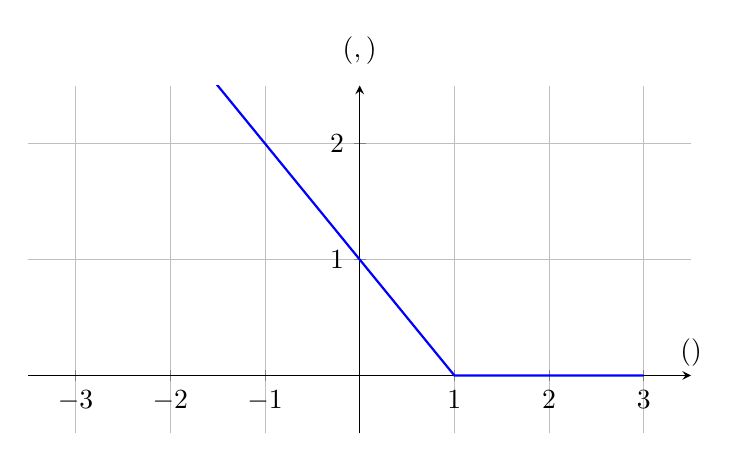
\begin{tikzpicture}
    \begin{axis}[
        axis lines=middle,
        xlabel={$\truelabel\hypothesis(\featurevec)$},
        ylabel={$\lossfunc{(\featurevec,\truelabel)}{\hypothesis}$},
 	xlabel style={at={(axis description cs:1.,0.3)}, anchor=north},  % Adjusted to be relative to axis end
        ylabel style={at={(axis description cs:0.5,1.1)}, anchor=center}, % Corrected to vertical position, rotated for readability
        xmin=-3.5, xmax=3.5,
        ymin=-0.5, ymax=2.5,
        xtick={-3, -2, -1, 0, 1, 2, 3},
        ytick={0, 1, 2},
        domain=-3:3,
        samples=100,
        width=10cm, height=6cm,
        grid=both,
        major grid style={line width=.2pt, draw=gray!50},
        minor grid style={line width=.1pt, draw=gray!20},
        legend pos=south west % Positions legend at the bottom left
    ]
        \addplot[blue, thick] {max(0, 1-x)};
     %   \addlegendentry{$\max(0, 1-x)$}
    \end{axis}
\end{tikzpicture}
	%	\end{figure} 
		\end{center}
	    A regularized variant of the hinge loss is used by the \gls{svm} \cite{LampertNowKernel}. 	    
		},first={hinge loss},text={hinge loss}}

\newglossaryentry{iidasspt}{name={i.i.d.\ assumption}, description={The i.i.d.\ assumption\index{i.i.d.} interprets \gls{datapoint}s of a \gls{dataset} 
		as the realizations of \gls{iid} \gls{rv}s.},first={i.i.d.\ assumption},text={i.i.d.\ assumption} }

\newglossaryentry{hypospace}{name={hypothesis space}, description={Every\index{hypothesis space} 
		practical ML method uses a hypothesis space (or \gls{model}) $\hypospace$. The hypothesis space 
		of an ML method is a subset of all possible maps from the \gls{featurespace} to the \gls{labelspace}. 
		The design choice of the hypothesis space should take into account available computational resources and 
		statistical aspects. If the computational infrastructure allows for efficient matrix operations, and there 
		is a (approximately) linear relation between \gls{feature}s and \gls{label}, a useful choice for the 
		hypothesis space might be the \gls{linmodel}.},first={hypothesis space},text={hypothesis space} }
	
\newglossaryentry{model}{name={model}, description={In the context of ML methods, 
		the term \emph{model} typically refers to the \gls{hypospace} used by an 
		ML method \cite{ShalevMLBook,MLBasics}.},first={model},text={model} }

\newglossaryentry{modelparams}{name={model parameters}, 
	description={Model parameters\index{model parameters} are quantities that 
	are used to select a specific \gls{hypothesis} map from a \gls{model}. 
	We can think of model parameters as a unique identifier for a \gls{hypothesis} 
	map, similar to how a social security number identifies a person in Finland.},
	first={model parameters},text={model parameters} }

\newglossaryentry{ai}{name={artificial intelligence}, description={
		Artificial intelligence \index{artificial intelligence} refers to systems that behave rationally in the sense of 
		maximizing a long-term \gls{reward}. The ML-based approach to AI is to train a \gls{model} that allows 
		the predict optimal actionsfor a given observed state of the environment. The choice of \gls{lossfunc}
		sets AI applications apart from more basic ML applications. AI systems rarely have access to a labelled 
		\gls{trainset} that allows the average \gls{loss} to be measured for any possible choice of \gls{modelparams}. 
		Instead, AI systems use observed reward signals to obtain an (point-wise) estimate for the 
		\gls{loss} incurred by the current choice of \gls{modelparams}.},first={artificial intelligence (AI)},text={AI} }

\newglossaryentry{reward}{name={reward}, description={Some\index{reward} observed (or measured) quantity that allows to estimate the \gls{loss} 
	incurred by the \gls{prediction} (or decision) of a \gls{hypothesis} $h(\featurevec)$. For example, 
	in a ML application to self-driving vehicles, $h(\featurevec)$ could represent the current steering 
	direction of vehicle. We could construct a reward from the measurements of a collision sensor that 
	indicate if the vehicle is moving towards an obstacle. We define a low reward for the steering direction 
	$h(\featurevec)$ if the vehicle moves dangerously towards an obstacle.},
	first={reward}, text={reward}} 

\newglossaryentry{hardclustering}{name={hard clustering}, description={Hard clustering\index{hard clustering} 
		refers to the task of partitioning a given set of \gls{datapoint}s into (a few) non-overlapping \gls{cluster}s. 
		The most widely used hard clustering method is \gls{kmeans}.},first={hard clustering},text={hard clustering} }
	
\newglossaryentry{softclustering}{name={soft clustering}, description={Soft clustering\index{soft clustering} 
		refers to the task of partitioning a given set of \gls{datapoint}s into (a few) overlapping clusters. 
		Each \gls{datapoint} is assigned to several different \gls{cluster}s with varying \gls{dob}. Soft clustering 
		methods determine the \gls{dob} (or soft \gls{cluster} assignment) for each \gls{datapoint} and each \gls{cluster}.
		A principled approach to soft \gls{clustering} is by interpreting \gls{datapoint}s as \gls{iid} \gls{realization}s 
		of a \gls{gmm}. We then obtain a natural choice for the \gls{dob} as the conditional 
		probability of a \gls{datapoint} belonging to a specific mixture component.},first={soft clustering},text={soft clustering} }
	
\newglossaryentry{clustering}{name={clustering}, description={Clustering\index{clustering} methods decompose a given 
		set of \gls{datapoint}s into a few subsets, which are referred to as \gls{cluster}s. 
		Each \gls{cluster} consists of \gls{datapoint}s that are more similar to each 
		other than to \gls{datapoint}s outside the \gls{cluster}. Different clustering methods 
		use different measures for the similarity between \gls{datapoint}s and different 
		forms of \gls{cluster} representations. The clustering method \gls{kmeans} uses the 
		average \gls{feature} vector (\emph{cluster mean}) of a \gls{cluster} as its representative. 
		A popular \gls{softclustering} method based on \gls{gmm} represents 
		a \gls{cluster} by a \gls{mvndist}.},first={clustering},text={clustering} }
	
\newglossaryentry{cluster}{name={cluster}, description={A\index{cluster} \gls{cluster} is a subset of 
		\gls{datapoint}s that are more similar to each other than to the \gls{datapoint}s outside the \gls{cluster}. 
		The quantitative measure of similarity between \gls{datapoint}s is a design choice. If \gls{datapoint}s 
		are characterized by Euclidean \gls{feature} vectors $\featurevec \in \mathbb{R}^{\nrfeatures}$, 
		we can define the similarity between two \gls{datapoint}s via the Euclidean distance between 
		their \gls{feature} vectors.},first={cluster},text={cluster} }

%\newglossaryentry{softclustering}{name={soft clustering}, description={Soft clustering methods determine, for each \gls{datapoint} within a dataset, 
%		a soft cluster assignment or the degree of belonging to a particular cluster.},first={soft clustering},text={soft clustering} }


\newglossaryentry{huberloss}{name={Huber loss}, description={The\index{Huber loss} 
		Huber \gls{loss} unifies the \gls{sqerrloss} and the absolute error \gls{loss}.},first={Huber loss},text={Huber loss} }

\newglossaryentry{svm}{name={support vector machine}, description={The\index{support vector machine} 
		support vector machine (SVM) is a binary \gls{classification} method that learns a linear \gls{hypothesis} map. 
		Thus, like \gls{linreg} and \gls{logreg}, it is also an instance of \gls{erm} for the \gls{linmodel}. However, 
		the support vector machine uses a different \gls{lossfunc} than those methods. As illustrated in Figure \ref{fig_svm_gls}, 
		it aims to maximally separate \gls{datapoint}s from the two different classes in the \gls{feature} space 
		(\emph{maximum margin principle}). Maximizing this separation is equivalent to minimizing a regularised 
		variant of the \gls{hingeloss} \eqref{equ_hinge_loss_gls} \cite{LampertNowKernel,Cristianini_Shawe-Taylor_2000,BishopBook}
		\begin{figure}[htbp]
			\begin{center}
				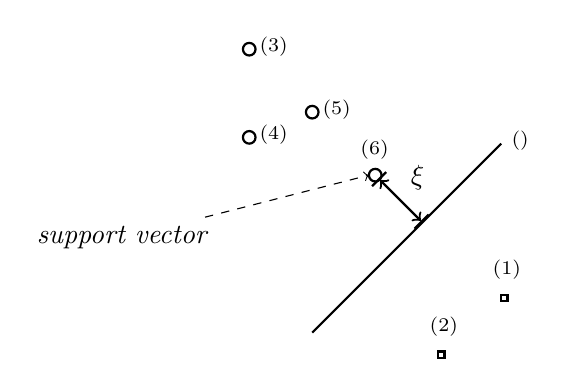
\begin{tikzpicture}[auto,scale=0.8]
					%\draw [thick] (0,-3) rectangle (4,4) node [anchor=east,above] {$\featurespace$} ;
					\draw [thick] (1,2) circle (0.1cm)node[anchor=west] {\hspace*{0mm}$\featurevec^{(5)}$};
					\draw [thick] (0,1.6) circle (0.1cm)node[anchor=west] {\hspace*{0mm}$\featurevec^{(4)}$};
					\draw [thick] (0,3) circle (0.1cm)node[anchor=west] {\hspace*{0mm}$\featurevec^{(3)}$};
					\draw [thick] (2,1) circle (0.1cm)node[anchor=east,above] {\hspace*{0mm}$\featurevec^{(6)}$};
					\node[] (B) at (-2,0) {\emph{support vector}};
					\draw[->,dashed] (B) to (1.9,1) ; 
					\draw [|<->|,thick] (2.05,0.95)  -- (2.75,0.25)node[pos=0.5] {$\xi$} ; 
					\draw [thick] (1,-1.5) -- (4,1.5) node [right] {$\hypothesis^{(\weights)}$} ; 
					\draw [thick] (3,-1.9) rectangle ++(0.1cm,0.1cm) node[anchor=west,above]  {\hspace*{0mm}$\featurevec^{(2)}$};
					\draw [thick] (4,.-1) rectangle ++(0.1cm,0.1cm) node[anchor=west,above] {\hspace*{0mm}$\featurevec^{(1)}$};
				\end{tikzpicture}
				\caption{The \gls{svm} learns a hypothesis (or classifier) $\hypothesis^{(\weights)}$ with 
					minimum average soft-margin \gls{hingeloss}. Minimizing this \gls{loss} is equivalent 
					to maximizing the margin $\xi$ between the \gls{decisionboundary} of $\hypothesis^{(\weights)}$ 
					and each class of the \gls{trainset}.}
				\label{fig_svm_gls}
			\end{center}
		\end{figure}
		The above basic variant of SVM is only useful if the \gls{datapoint}s from different categories can be  
		(approximately) linearly separated. For an ML application where the categories are not 
		%linearly separable based on the the original (raw) \gls{feature}s it is possible to apply the SVM 
		%to transformed \gls{feature}s. These transformed \gls{feature}s can be obtained by applying a \gls{featuremap} 
		derived from a \gls{kernel}.
},first={support vector machine (SVM)},text={SVM} }

\newglossaryentry{eigenvalue}{name={eigenvalue}, description={We refer to a 
		number $\lambda \in \mathbb{R}$ as an eigenvalue of a square matrix $\mathbf{A} \in \mathbb{R}^{\featuredim \times \featuredim}$ 
		if there is a non-zero vector $\vx \in \mathbb{R}^{\featuredim} \setminus \{ \mathbf{0} \}$ such that $\mathbf{A} \vx = \lambda \vx$. },first={eigenvalue},text={eigenvalue} }
	
\newglossaryentry{eigenvector}{name={eigenvector}, description={An\index{eigenvector} 
		eigenvector of a matrix $\mathbf{A} \in \mathbb{R}^{\featuredim \times \featuredim}$ 
		is a non-zero vector $\vx \in \mathbb{R}^{\featuredim} \setminus \{ \mathbf{0} \}$ 
		such that $\mathbf{A} \vx = \lambda \vx$ with some \gls{eigenvalue} $\lambda$.},first={eigenvector},text={eigenvector} }

\newglossaryentry{evd}{name={eigenvalue decomposition}, 
	description={The\index{eigenvalue decomposition} \gls{eigenvalue} 
		decomposition for a square matrix $\mA \in \mathbb{R}^{\dimlocalmodel \times \dimlocalmodel}$ 
		is a factorization of the form 
		$$\mA = \mathbf{V} {\bm \Lambda} \mathbf{V}^{-1}.$$ 
		The columns of the matrix $\mV = \big( \vv^{(1)},\ldots,\vv^{(\dimlocalmodel)} \big)$ are the 
		\gls{eigenvector}s of the matrix $\mV$. The diagonal matrix 
		${\bm \Lambda} = {\rm diag} \big\{ \eigval{1},\ldots,\eigval{\dimlocalmodel} \big\}$ 
		contains the \gls{eigenvalue}s $\eigval{\featureidx}$ corresponding to the \gls{eigenvector}s $\vv^{(\featureidx)}$. 
		Note that the above decomposition exists only if the matrix $\mA$ is diagonalizable.},first={eigenvalue decomposition (EVD)},text={EVD} }

\newglossaryentry{svd}{name={singular value decomposition}, 
  	description={The\index{singular value decomposition} singular value 
  		decomposition for a matrix $\mA \in \mathbb{R}^{\samplesize \times \dimlocalmodel}$ 
		is a factorization of the form 
		$$\mA = \mathbf{V} {\bm \Lambda} \mathbf{U}^{T},$$ 
		with orthonormal matrices $\mV \in \mathbb{R}^{\samplesize \times \samplesize}$ 
		and $\mU \in \mathbb{R}^{\dimlocalmodel \times \dimlocalmodel}$ \cite{GolubVanLoanBook}. 
		The matrix ${\bm \Lambda} \in \mathbb{R}^{\samplesize \times \dimlocalmodel}$ is 
		only non-zero along the main diagonal, whose entries $\Lambda_{\featureidx,\featureidx}$ 
		are non-negative and referred to as singular values.
	},first={singular value decomposition (SVD)},text={SVD} }


\newglossaryentry{tv}{name={total variation}, description={See \gls{gtv}.},
	first={total variation},text={total variation} }

 \newglossaryentry{cvxclustering}{name={convex clustering}, 
 	description={Consider\index{convex clustering} a \gls{dataset} 
 	$\featurevec^{(1)},\ldots,\featurevec^{(\samplesize)} \in \mathbb{R}^{\nrfeatures}$. 
 	Convex clustering learns vectors $\weights^{(1)},\ldots,\weights^{(\samplesize)}$ by 
 	minimizing 
 	$$ \sum_{\sampleidx=1}^{\samplesize} \normgeneric{\featurevec^{(\sampleidx)} - \weights^{(\sampleidx)}}{2}^2 + 
 	\regparam \sum_{\nodeidx,\nodeidx' \in \nodes} \normgeneric{\weights^{(\nodeidx)} - \weights^{(\nodeidx')}}{p}.$$ 
	Here, $ \normgeneric{\vu}{p} \defeq \big( \sum_{\featureidx=1}^{\dimlocalmodel} |u_{\featureidx}|^{p} \big)^{1/p}$ 
	denotes the $p$-norm (for $p\geq1$).  
	It turns out that many of the optimal vectors $\widehat{\weights}^{(1)},\ldots,\widehat{\weights}^{(\samplesize)}$ 
	coincide. A cluster then consists of those \gls{datapoint}s $\sampleidx \in \{1,\ldots,\samplesize\}$ 
	with identical $\widehat{\weights}^{(\sampleidx)}$ \cite{JMLR:v22:18-694,Pelckmans2005}. 
 	  },
 		first={convex clustering},text={convex clustering} }


\newglossaryentry{gdmethods}{name={gradient-based method}, 
	description={Gradient-based\index{gradient-based methods} 
		methods are iterative techniques for finding the minimum (or maximum) 
		of a \gls{differentiable} objective function of the \gls{modelparams}. These 
		methods construct a sequence of approximations to an optimal choice for 
		\gls{modelparams} that results in a minimum (or maximum) value of the \gls{objfunc}. 
		As their name indicates, gradient-based methods use the \gls{gradient}s of the \gls{objfunc} 
		evaluated during previous iterations to construct new (hopefully) improved \gls{modelparams}. 
		One important example of a gradient-based method is \gls{gd}.},
		first={gradient-based methods},text={gradient-based methods} }

\newglossaryentry{sgd}{name={subgradient descent}, description={Subgradient\index{subgradient descent} 
		descent is a generalization of \gls{gd} that does not require differentiability of the 
		function to be minimized. This generalization is obtained by replacing the concept 
		of a \gls{gradient} with that of a sub-gradient. Similar to \gls{gradient}s, also sub-gradients 
		allow to construct local approximations of an objective function. The objective function 
		might be the \gls{emprisk} $\emperror\big( \hypothesis^{(\weights)} \big| \dataset \big)$ viewed 
		as a function of the \gls{modelparams} $\weights$ that select a \gls{hypothesis} $\hypothesis^{(\weights)} \in \hypospace$.},first={subgradient descent},text={subgradient descent} }
	
\newglossaryentry{stochGD}{name={stochastic gradient descent}, description={Stochastic\index{stochastic gradient descent} 
		\gls{gd} is obtained from \gls{gd} by replacing the \gls{gradient} of the \gls{objfunc} 
		with a stochastic approximation. A main application of stochastic gradient descent 
		is to implement \gls{erm} for a parametrized \gls{model} and a \gls{trainset} $\dataset$ 
		is either very large or not readily available (e.g., when \gls{datapoint}s are stored 
		in a database distributed all over the planet). To evaluate the \gls{gradient} of the 
		\gls{emprisk} (as a function of the \gls{modelparams} $\weights$), 
		we need to compute a sum $\sum_{\sampleidx=1}^{\samplesize} \nabla_{\weights} \lossfunc{\datapoint^{(\sampleidx)}}{\weights}$  
		over all \gls{datapoint}s in the \gls{trainset}. We obtain a stochastic 
		approximation to the \gls{gradient} by replacing the sum $\sum_{\sampleidx=1}^{\samplesize} \nabla_{\weights} \lossfunc{\datapoint^{(\sampleidx)}}{\weights}$ 
		with a sum $\sum_{\sampleidx \in \batch} \nabla_{\weights} \lossfunc{\datapoint^{(\sampleidx)}}{\weights}$ 
		over a randomly chosen subset $\batch \subseteq \{1,\ldots,\samplesize\}$ (see Figure \ref{fig_sgd_approx}). 
		We often refer to these randomly chosen \gls{datapoint}s as a \emph{batch}. 
		The batch size $|\batch|$ is an important parameter of stochastic \gls{gd}. 
		Stochastic \gls{gd} with $|\batch|> 1$ is referred to as mini-batch stochastic \gls{gd} \cite{Bottou99}. 		
		\begin{figure}
			\centering
			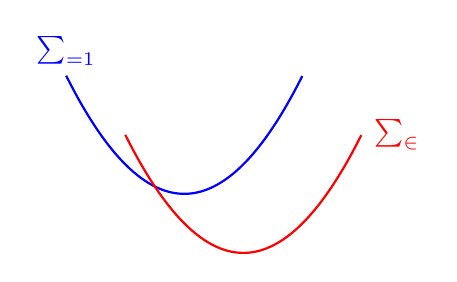
\begin{tikzpicture}[scale=1.5, >=stealth]
% Axes
				%\draw[->] (-1, 0) -- (4, 0) node[right] {$w$};
				%\draw[->] (0, -0.5) -- (0, 4) node[above] {};
% First quadratic function: f(w)
				\draw[thick, blue, domain=0.5:2.5, samples=100] plot (\x, {(\x-1.5)^2 + 1});
				\node[blue,above] at (0.5, 2) {$\sum_{\sampleidx=1}^{\samplesize}$};
% Second quadratic function: f'(w)
				\draw[thick, red, domain=1:3, samples=100] plot (\x, {(\x-2)^2 + 0.5});
				\node[red] at (3.3, 1.5) {$\sum_{\sampleidx \in \batch}$};
% Labels
			\end{tikzpicture}
		\caption{Stochastic \gls{gd} for \gls{erm} approximates the \gls{gradient} 
		$\sum_{\sampleidx=1}^{\samplesize} \nabla_{\weights} \lossfunc{\datapoint^{(\sampleidx)}}{\weights}$ 
		by replacing the 
		sum over all \gls{datapoint}s in the \gls{trainset} (indexed by $\sampleidx=1,\ldots,\samplesize$) 
		with a sum over a randomly chosen subset $\batch \subseteq \{1,\ldots,\samplesize\}$.\label{fig_sgd_approx}}
		\end{figure}
},first={stochastic gradient descent (SGD)},text={SGD} }


\newglossaryentry{onlineGD}{name={online GD}, description={
Consider \index{online GD} an ML method that learns \gls{modelparams} 
$\weights$ from some \gls{paramspace} $\paramspace \subseteq \mathbb{R}^{\dimlocalmodel}$. 
The learning uses \gls{datapoint}s $\datapoint^{(\timeidx)}$ that arrive at consecutive time-instants $\timeidx=1,2,\ldots$. 
Let us interpret the \gls{datapoint}s $\datapoint^{(\timeidx)}$ as \gls{iid} copies 
of a \gls{rv} $\datapoint$. The \gls{risk} $\expect\{ \lossfunc{\datapoint}{\weights} \}$ of a 
\gls{hypothesis} $\hypothesis^{(\weights)}$ can then (under mild conditions) be obtained as the limit 
$\lim_{T\rightarrow \infty} (1/T)\sum_{\timeidx=1}^{T} \lossfunc{\datapoint^{(\timeidx)}}{\weights}$. 
We might use this limit as the \gls{objfunc} for learning the \gls{modelparams} $\weights$. 
Unfortunately, this limit can only be evaluated if we wait infinitely long in order to collect all \gls{datapoint}s. 
Some ML applications require methods that learn \emph{online}: as soon as a new \gls{datapoint} $\datapoint^{(\timeidx)}$ 
arrives at time $\timeidx$, we update the current \gls{modelparams} $\weights^{(\timeidx)}$. Note that 
the new \gls{datapoint} $\datapoint^{(\timeidx)}$ contributes the component $\lossfunc{\datapoint^{(\timeidx)}}{\weights}$ 
to the \gls{risk}. As it name suggests, online GD updates $\weights^{(\timeidx)}$ via a (projected) \gls{gradstep}
\begin{equation} 
\label{equ_def_ogd}
 \weights^{(\timeidx+1)} \defeq \projection{\paramspace}{\weights^{(\timeidx)} - \lrate_{\timeidx} \nabla_{\weights} \lossfunc{\datapoint^{(\timeidx)}}{\weights}}. 
\end{equation} 
Note that \eqref{equ_def_ogd} is a \gls{gradstep} for the current component $\lossfunc{\datapoint^{(\timeidx)}}{\cdot}$ 
of the \gls{risk}. The update \eqref{equ_def_ogd} ignores all the previous components $\lossfunc{\datapoint^{(\timeidx')}}{\cdot}$, 
for $\timeidx' < \timeidx$. It might therefore happen that, compared to $\weights^{(\timeidx)}$, the updated \gls{modelparams} 
$\weights^{(\timeidx+1)}$ increase the retrospective average \gls{loss} $\sum_{\timeidx'=1}^{\timeidx-1} \lossfunc{\datapoint^{(\timeidx')}}{\cdot}$. 
However, for a suitably chosen \gls{learnrate} $\lrate_{\timeidx}$, online GD can be shown 
to be optimal in practically relevant settings. By optimal, we mean that the \gls{modelparams} 
$\weights^{(T+1)}$ delivered by online GD after observing $T$ \gls{datapoint}s $\datapoint^{(1)},\ldots, \datapoint^{(T)}$ 
are at least as good as those delivered by any other learning method \cite{HazanOCO,GDOptimalRakhlin2012}. 
\begin{figure}
	\begin{center}
\begin{tikzpicture}[x=1.5cm,scale=1.5, every node/.style={font=\footnotesize}]
	% Axes
	\draw[->] (0.5, 0) -- (5.5, 0) node[below] {};
	%\draw[->] (0, -0.5) -- (0, 3) node[left] {Value};
	% Labels for time steps
	\foreach \x in {1, 2, 3, 4, 5} {
		\draw (\x, 0.1) -- (\x, -0.1) node[below] {$t=\x$};
	}
	% Data points (black circles)
	\foreach \x/\y in {1/2.5, 2/1.8, 3/2.3, 4/1.5, 5/2.0} {
		\fill[black] (\x, \y) circle (2pt) node[above right] {$\datapoint^{(\x)}$};
	}
	% Model parameters (blue circles)
	\foreach \x/\y in {1/1.0, 2/1.6, 3/1.8, 4/2.2, 5/1.9} {
		\fill[blue] (\x, \y) circle (2pt) node[below left] {$\weights^{(\x)}$};
	}
	% Connecting lines (model tracking data)
	\foreach \x/\y/\z in {1/2.5/1.0, 2/1.8/1.6, 3/2.3/2.0, 4/1.5/1.8, 5/2.0/1.9} {
		\draw[dashed, gray] (\x, \y) -- (\x, \z);
	}
	% Legend
	% \node[draw, fill=white] at (4.5, 2.7) {
	% 	\begin{tabular}{@{}ll@{}}
	% 		\textcolor{black}{$\bullet$} & Data Point ($d_t$) \\
	% 		\textcolor{blue}{$\bullet$} & Model Parameter ($\theta_t$) \\
	% 		\textcolor{gray}{\rule{1cm}{0.5pt}} & Gradient Update
	% 	\end{tabular}
	%};
	\end{tikzpicture}
\end{center} 
\caption{An instance of online GD that updates the \gls{modelparams} $\weight^{(\timeidx)}$ 
using the \gls{datapoint} $\datapoint^{(\timeidx)} = \feature^{(\timeidx)}$ arriving at time $\timeidx$. 
This instance uses the \gls{sqerrloss} $\lossfunc{\datapoint^{(\timeidx)}}{\weight} = (\feature^{(\timeidx)} - \weight)^{2}$.
}
\end{figure}},
first={online gradient descent (online GD)},text={online GD}}

\newglossaryentry{pca}{name={principal component analysis (PCA)}, description={Principal\index{principal component analysis} 
		component analysis determines a linear \gls{featuremap} such that the new \gls{feature}s 
		allow to reconstruct the original \gls{feature}s with the minimum reconstruction error \cite{MLBasics}.},first={principal component analysis (PCA)},text={PCA} }
	
\newglossaryentry{loss}{name={loss}, description={ML\index{loss} methods use a 
		\gls{lossfunc} $\lossfunc{\datapoint}{\hypothesis}$ to measure the error incurred 
		by applying a specific \gls{hypothesis} to a specific \gls{datapoint}. With 
		slight abuse of notation, we use the term \emph{loss} for both, the \gls{lossfunc} $\loss$ 
		itself and the specific value $\lossfunc{\datapoint}{\hypothesis}$ for a \gls{datapoint} $\datapoint$ 
		and \gls{hypothesis} $\hypothesis$.},first={loss},text={loss} }

\newglossaryentry{lossfunc}{name={loss function}, description={A\index{loss function} loss function is a map 
		$$\lossfun: \featurespace \times \labelspace \times \hypospace \rightarrow \mathbb{R}_{+}: \big( \big(\featurevec,\truelabel\big),
		 \hypothesis\big) \mapsto  \lossfunc{(\featurevec,\truelabel)}{\hypothesis}.$$
		It assigns a pair, consisting of a \gls{datapoint}, with features $\featurevec$ 
		and label $\truelabel$, and a \gls{hypothesis} $\hypothesis \in \hypospace$, a 
		non-negative real number (the \emph{loss}) $\lossfunc{(\featurevec,\truelabel)}{\hypothesis}$. The 
		value $\lossfunc{(\featurevec,\truelabel)}{\hypothesis}$ quantifies the discrepancy 
		between the true \gls{label} $\truelabel$ and the \gls{prediction} $\hypothesis(\featurevec)$. 
		Lower (closer to zero) values $\lossfunc{(\featurevec,\truelabel)}{\hypothesis}$ indicate a smaller 
		discrepancy between \gls{prediction} $\hypothesis(\featurevec)$ and label $\truelabel$. 
		Figure \ref{fig_loss_function_gls} depicts a \gls{lossfunc} for a given \gls{datapoint}, 
		with \gls{feature}s $\featurevec$ and label $\truelabel$, as a function of the \gls{hypothesis} $\hypothesis \in \hypospace$. 
		\begin{figure}[htbp]
			\begin{center}
				\begin{tikzpicture}[scale = 0.7]
					\begin{axis}
						[%grid, 
						axis x line=center,
						axis y line=center,
						%	xtick={-2,-1,...,2},
						%	ytick={0,1,...,2},
						xlabel={},
						%	ylabel={\hspace*{3mm} loss $\lossfun$},
						xlabel style={below right},
						ylabel style={above right},
						xtick=\empty,
						ytick=\empty,
						xmin=-4,
						xscale = 1.4, 
						xmax=4,
						ymin=-0.5,
						ymax=2.5
						]
						\addplot [smooth, ultra thick] table [x=a, y=b, col sep=comma] {assets/logloss.csv};    
					\end{axis}
					\node [above] at (1,5) {$\lossfunc{(\featurevec,\truelabel)}{\hypothesis}$};
					\node [above] at (10,1) {\gls{hypothesis} $\hypothesis$};
						\node [right] at (4,6) {\gls{loss}};
				\end{tikzpicture}
			\end{center}
			\vspace*{-7mm}
			\caption{Some \gls{lossfunc} $\lossfunc{(\featurevec,\truelabel)}{\hypothesis}$ for a fixed \gls{datapoint}, with 
				\gls{feature} vector $\featurevec$ and \gls{label} $\truelabel$, and varying \gls{hypothesis} $\hypothesis$. 
				ML methods try to find (learn) a \gls{hypothesis} that incurs minimal \gls{loss}.}
			\label{fig_loss_function_gls}
	\end{figure}
 },first={loss function},text={loss function} }

\newglossaryentry{decisiontree}{name={decision tree}, description={A\index{decision tree} 
		decision tree is a flow-chart-like representation of a \gls{hypothesis} map $\hypothesis$. 
		More formally, a decision tree is a directed graph containing a root node that reads 
		in the feature vector $\featurevec$ of a \gls{datapoint}. The root node then forwards 
		the \gls{datapoint} to one of its children nodes based on some elementary test on the \gls{feature}s $\featurevec$. 
		If the receiving children node is not a leaf node, i.e., it has itself children nodes, 
	  it represents another test. Based on the test result, the \gls{datapoint} is further 
	  pushed to one of its descendants. This testing and forwarding of the \gls{datapoint} is continued 
	  until the \gls{datapoint} ends up in a leaf node (having no children nodes). 
	  %Each leaf node corresponds to a \gls{decisionregion}, a subset of the \gls{featurespace} 
	  %mapped to the same output $\hypothesis(\featurevec)$.
	  }
	  ,first={decision tree},text={decision tree} }

\newglossaryentry{API} 
{
	name={Application Programming Interface (API)},
	description={An\index{application programming interface} application programming 
		interface (API) is a precise specification of the services and resources 
		offered by software or hardware implementing that API.},
	first={application programming interface (API)},
	text={API}
}

\newglossaryentry{hilbertspace}{name={Hilbert space},description={A\index{Hilbert space} 
		Hilbert space is a linear vector space equipped with an inner product between 
		pairs of vectors. One important example of a Hilbert space is the \gls{euclidspace} 
		$\mathbb{R}^{\featuredim}$, for some dimension $\featuredim$, which consists of 
		Euclidean vectors $\vu = \big(u_{1},\ldots,u_{\featurelen}\big)^{T}$ along with the inner 
		product $\vu^{T} \vv$.},first={Hilbert space},text={Hilbert space}}



\newglossaryentry{sample}{name={sample},description={A\index{sample} 
		finite sequence (list) of \gls{datapoint}s $\datapoint^{(1)},\ldots,\datapoint^{(\sampleidx)}$ that 
		is obtained or interpreted as the realizations of $\samplesize$ \gls{iid} \gls{rv}s 
		with the common \gls{probdist} $p(\datapoint)$. The length $\samplesize$ of 
		the sequence is referred to as the \gls{samplesize}.},first={sample},text={sample}}
	
\newglossaryentry{samplesize}
{name=sample size,
	description={The\index{sample size} number of individual \gls{datapoint}s 
		contained in a \gls{dataset} obtained as the \gls{realization}s of \gls{iid} \gls{rv}s with 
		common \gls{probdist}.},first={sample size},text={sample size}
}

\newglossaryentry{ann}
{name=artificial neural network,
	description={An\index{artificial neural network} artificial neural network is a 
		graphical (signal-flow) representation of a map from \gls{feature}s of 
		a \gls{datapoint} at its input to a \gls{prediction} for the \gls{label} 
		as its output.},first={artificial neural network (ANN)},text={ANN}
}

\newglossaryentry{randomforest}
{name=random forest,
	description={A\index{random forest} random forest is a set (ensemble) of different \gls{decisiontree}s. 
		Each of these \gls{decisiontree}s is obtained by fitting a perturbed copy of 
		the original \gls{dataset}.},first = {random forest}, text={random forest}
}

\newglossaryentry{bagging}{name={bagging},description={Bagging\index{bagging} (or \emph{bootstrap aggregation}) 
		is a generic technique to improve (the robustness of) a given ML method. The idea is to use the \gls{bootstrap} 
		to generate perturbed copies of a given \gls{dataset} and then to learn a separate \gls{hypothesis} for 
		each copy. We then predict the \gls{label} of a \gls{datapoint} by combining or aggregating the individual 
		\gls{prediction}s of each separate \gls{hypothesis}. For \gls{hypothesis} maps delivering numeric \gls{label} 
		values, this aggregation could be implemented by computing the average of individual \gls{prediction}s.},first={bootstrap aggregation (bagging)},text={bagging}}

\newglossaryentry{gd}{name={gradient descent (GD)},description={Gradient\index{gradient descent} 
		descent is an iterative method for finding the minimum of a \gls{differentiable} function $f(\weights)$ 
		of a vector-valued argument $\weights \in \mathbb{R}^{\featurelen}$. Consider a current guess or 
		approximation $\weights^{(\itercntr)}$ for minimum. We would like to find a new (better) vector $\weights^{(\itercntr+1)}$ 
		that has a smaller objective value $f(\weights^{(\itercntr+1)}) < f\big(\weights^{(\itercntr)}\big)$ than 
		the current guess $\weights^{(\itercntr)}$. We can achieve this typically by using a gradient step
		\begin{equation} 
			\label{equ_def_GD_step}
			\weights^{(\itercntr\!+\!1)} = \weights^{(\itercntr)} - \lrate \nabla f(\weights^{(\itercntr)})
		\end{equation} 
		with a sufficiently small \gls{stepsize} $\lrate>0$. Figure \ref{fig_basic_GD_step} illustrates the effect of 
		a single \gls{gd} step \eqref{equ_def_GD_step}.
		\begin{figure}[htbp]
			\begin{center}
				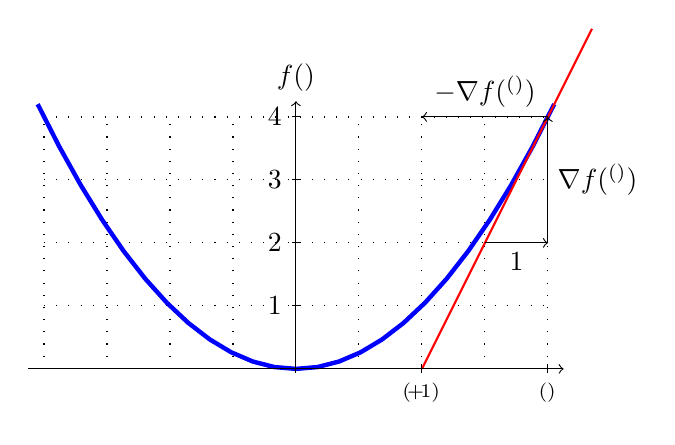
\begin{tikzpicture}[scale=0.8]
					\draw[loosely dotted] (-4,0) grid (4,4);
					\draw[blue, ultra thick, domain=-4.1:4.1] plot (\x,  {(1/4)*\x*\x});
					\draw[red, thick, domain=2:4.7] plot (\x,  {2*\x - 4});
					\draw[<-] (4,4) -- node[right] {$\nabla f(\weights^{(\itercntr)})$} (4,2);
					\draw[->] (4,4) -- node[above] {$-\lrate \nabla f(\weights^{(\itercntr)})$} (2,4);
					\draw[<-] (4,2) -- node[below] {$1$} (3,2) ;
					\draw[->] (-4.25,0) -- (4.25,0) node[right] {$\weights$};
					\draw[->] (0,-2pt) -- (0,4.25) node[above] {$f(\weights)$};
					\draw[shift={(0,0)}] (0pt,2pt) -- (0pt,-2pt) node[below] {$\overline{\weights}$};
					\draw[shift={(4,0)}] (0pt,2pt) -- (0pt,-2pt) node[below] {$\weights^{(\itercntr)}$};
					\draw[shift={(2,0)}] (0pt,2pt) -- (0pt,-2pt) node[below] {$\weights^{(\itercntr\!+\!1)}$};
					\foreach \y/\ytext in {1/1, 2/2, 3/3, 4/4}
					\draw[shift={(0,\y)}] (2pt,0pt) -- (-2pt,0pt) node[left] {$\ytext$};  
				\end{tikzpicture}
			\end{center}
			\caption{A single gradient step \eqref{equ_def_GD_step} towards the minimizer $\overline{\weights}$ of $f(\weights)$.}
			\label{fig_basic_GD_step}
		\end{figure}
%		
		},first={gradient descent (GD)},text={GD}}

\newglossaryentry{abserr}{name={absolute error loss},description={
			Consider a \gls{datapoint} with \gls{feature}s $\featurevec \in \featurespace$ and 
			numeric \gls{label} $\truelabel \in \mathbb{R}$. 
			The absolute error loss \index{absolute error loss} incurred by 
			a \gls{hypothesis} $\hypothesis: \featurespace \rightarrow \mathbb{R}$ 
			is defined as $|\truelabel - \hypothesis(\featurevec)|$.},
			first={absolute error loss},text={absolute error loss}}

\newglossaryentry{device}{name={device},description={
				Any physical system that can be used to store and process \gls{data}. In the context of ML, 
				we typically mean a computer that is able to read in \gls{datapoint}s from different 
				sources and, in turn, to train an ML \gls{model} using these \gls{datapoint}s.},
				first={device},text={device}}

\newglossaryentry{llm}{name={Large Language Model},description={
	Large Language Models (LLMs) is an umbrella term for ML methods 
	that process and generate human-like text. These methods typically 
	use \gls{deepnet}s with billions (or even trillions) of parameters. 
	A widely used choice for the network architecture is referred to as 
	Transformers \cite{vaswani2017attention}. The training of LLMs is often  
	based on the task of predicting a few words that are intentionally removed 
	from a large text corpus. Thus, we can construct labelled \gls{datapoint}s 
	simply by selecting some words of a text as \gls{label}s and the remaining 
	words as \gls{feature}s of \gls{datapoint}s. This construction requires 
	very little human supervision and allows for generating sufficiently 
	large \gls{trainset}s for LLMs.},
					first={Large Language Model (LLM)},text={LLM}}


\newglossaryentry{huberreg}{name={Huber regression},description={
			Huber regression\index{Huber regression} refers \gls{erm}-based methods 
			that use the \gls{huberloss} as measure of the \gls{prediction} error. 
			Two important special cases of Huber regression are \gls{ladregression} and 
			\gls{linreg}. Tuning the threshold parameter of the \gls{huberloss} allows 
			to trade the robustness against outliers of abserr 
			against the smoothness of the \gls{sqerrloss}.},
			first={Huber regression},text={Huber regression}}


\newglossaryentry{ladregression}{name={least absolute deviation regression},description={
		Least\index{least absolute deviation regression} absolute deviation regression is 
		an instance of \gls{erm} using the absolute error loss. It is a special case of 
		\gls{huberreg}.},
		first={least absolute deviation regression},text={least absolute deviation regression}}

%\newglossaryentry{metric}{name={metric},description={We\index{metric} sometimes use \emph{metric} to refer to 
%		a \gls{lthat is used solely 
%	    for the final performance evaluation of a learnt hypothesis. The metric is typically a \gls{lossfunc} that 
%	    has a ``natural'' interpretation (such as the \gls{zerooneloss}) but is not a good choice to guide 
%	    the learning process, e.g., via \gls{erm}. For \gls{erm}, we typically prefer \gls{lossfunc}s that depend smoothly 
%	    on the (parameters of the) hypothesis. Examples for such smooth \gls{lossfunc}s include the \gls{sqerrloss} 
%	    and the \gls{logloss} \eqref{equ_log_loss_gls}.},first={metric},text={metric}}

\newglossaryentry{bayesrisk}{name={Bayes risk},description={Consider a \gls{probmodel} with 
joint \gls{probdist} $p(\featurevec,\truelabel)$ for the \gls{feature}s $\featurevec$ 
and \gls{label} $\truelabel$ of a \gls{datapoint}. The\index{Bayes risk} Bayes \gls{risk} 
is the minimum possible \gls{risk} that can be achieved by any \gls{hypothesis} 
$\hypothesis: \featurespace \rightarrow \labelspace$. Any \gls{hypothesis} that achieves 
the Bayes risk is referred to as a \gls{bayesestimator} \cite{LC}.},first={Bayes risk},text={Bayes risk}}
	
\newglossaryentry{bayesestimator}{name={Bayes estimator},description={Consider\index{Bayes estimator} 
a \gls{probmodel} with joint \gls{probdist} $p(\featurevec,\truelabel)$ for the \gls{feature}s $\featurevec$ and \gls{label} 
$\truelabel$ of a \gls{datapoint}. For a given \gls{lossfunc} $\lossfunc{\cdot}{\cdot}$, we refer to a \gls{hypothesis} 
$\hypothesis$ as a Bayes estimator if its \gls{risk} $\expect\{\lossfunc{\pair{\featurevec}{\truelabel}}{\hypothesis}\}$ is 
minimum \cite{LC}. Note that the property of a \gls{hypothesis} being a \gls{bayesestimator} depends on 
the underlying \gls{probdist} and the choice for the \gls{lossfunc} $\lossfunc{\cdot}{\cdot}$.},
		first={Bayes estimator},text={Bayes estimator}}


\newglossaryentry{weights}{name={weights},
	description={Consider\index{weights} a parameterized \gls{hypospace} $\hypospace$. 
		We\index{weights} use the term weights for numeric \gls{modelparams} that are 
		used to scale \gls{feature}s or their transformations in order to compute $\hypothesis^{(\weights)} \in \hypospace$. A \gls{linmodel} uses weights $\weights=\big(\weight_{1},\ldots,\weight_{\nrfeatures}\big)^{T}$ to compute 
		the linear combination $\hypothesis^{(\weights)}(\featurevec)= \weights^{T} \featurevec$. 
		Weights are also used in \gls{ann}s to form linear combinations of \gls{feature}s or the 
		outputs of neurons in hidden layers.},first={weights},text={weights}}
	
\newglossaryentry{probdist}{name={probability distribution},
	description={To\index{probability distribution} analyze ML methods it can be useful 
		to interpret \gls{datapoint}s as \gls{iid} \gls{realization}s of a \gls{rv}. The typical 
		properties of such \gls{datapoint}s are then governed by the probability distribution 
		of this \gls{rv}. The probability distribution of a binary \gls{rv} $\truelabel \in \{0,1\}$ 
		is fully specified by the probabilities $\prob{\truelabel = 0}$ and 
		$\prob{\truelabel=1}\!=\!1\!-\!\prob{\truelabel=0}$. The probability 
		distribution of a real-valued \gls{rv} $\feature \in \mathbb{R}$ might be specified 
		by a probability density function $p(\feature)$ such that $\prob{ \feature \in [a,b] } \approx  p(a) |b-a|$. 
	    In the most general case, a probability distribution is defined by a probability measure \cite{GrayProbBook,BillingsleyProbMeasure}.},first={probability distribution},text={probability distribution}}
    
    
\newglossaryentry{pdf}{name={probability density function (pdf)},
	description={The\index{probability density function} probability density function (pdf) $p(\feature)$ 
		of a real-valued \gls{rv} $\feature \in \mathbb{R}$ is a particular representation of its \gls{probdist}. 
		If the pdf exists, it can be used to compute the probability that $\feature$ takes on a value 
		from a (measurable) set $\mathcal{B} \subseteq \mathbb{R}$ via $\prob{\feature \in \mathcal{B}} = \int_{\mathcal{B}} p(\feature') d \feature'$ \cite[Ch. 3]{BertsekasProb}. The pdf of a vector-valued \gls{rv} $\featurevec \in \mathbb{R}^{\featuredim}$ (if it exists) 
        allows to compute the probability that $\featurevec$ falls into a (measurable) region $\mathcal{R}$ via 
        $\prob{\featurevec \in \mathcal{R}} = \int_{\mathcal{R}} p(\featurevec') d \feature_{1}' \ldots d \feature_{\featuredim}' $ \cite[Ch. 3]{BertsekasProb}.},
first={probability density function (pdf)},text={pdf}}


\newglossaryentry{parameters}{name={parameters},
	description={The\index{parameters} parameters of an ML \gls{model} are tunable 
		(learnable or adjustable) quantities that allow to choose between different \gls{hypothesis} maps. 
		For example, the linear model $\hypospace \defeq \{\hypothesis^{(\weights)}: \hypothesis^{(\weights)}(\feature)= \weight_{1} \feature + \weight_{2}\}$ 
		consists of all \gls{hypothesis} maps $\hypothesis^{(\weights)}(\feature)= \weight_{1} \feature + \weight_{2}$ 
		with a particular choice for the parameters $\weights = \big(\weight_{1},\weight_{2}\big)^{T} \in \mathbb{R}^{2}$. 
		Another example of parameters is the weights assigned to the connections 
		between neurons of an \gls{ann}.},first={parameters},text={parameters}}

\newglossaryentry{lln}{name={law of large numbers},
	description={The\index{law of large numbers} law of large numbers refers to the 
		convergence of the average of an increasing (large) number of \gls{iid} \gls{rv}s 
		to the \gls{mean} of their common \gls{probdist}. Different instances of the 
		law of large numbers are obtained using different notions of convergence \cite{papoulis}.},first={law of large numbers},text={law of large numbers}}
    
\newglossaryentry{stopcrit}{name={stopping criterion},
	description={Many\index{stopping criterion} ML methods use iterative algorithms that construct a 
		sequence of model parameters (such as the weights of a linear map or 
		the weights of an \gls{ann}) that (hopefully) converge to an optimal choice 
		for the model parameters. In practice, given finite computational 
		resources, we need to stop iterating after a finite number of repetitions. 
		A stopping criterion is any well-defined condition required for stopping 
		iterating.},first={stopping criterion},text={stopping criterion}}

\newglossaryentry{kCV}{name={$k$-fold cross-validation ($\nrfolds$-fold CV)},
	description={$k$-fold cross-validation\index{k-fold cross-validation} is a 
		method for learning and validating a \gls{hypothesis} using a given \gls{dataset}. 
		This method divides the \gls{dataset} evenly into $k$ subsets or \emph{folds} 
		and then executes $k$ repetitions of \gls{model} training (e.g., via \gls{erm}) and \gls{validation}. 
		Each repetition uses a different fold as the \gls{valset} and the remaining $k-1$ folds 
		as a \gls{trainset}. The final output is the average of the \gls{valerr}s obtained 
		from the $k$ repetitions.},first={$k$-fold cross-validation ($k$-fold CV)},text={$k$-fold CV}}
	
\newglossaryentry{renyidiv}{name={R\'enyi divergence}, 
	description={The R\'enyi divergence\index{R\'enyi divergence} measures the (dis-)similarity 
		between two \gls{probdist}s \cite{RenyiInfo95}.}, 
	first = {R\'enyi divergence}, text = {R\'enyi divergence}} 

\newglossaryentry{nonsmooth}{name={non-smooth},
	description={We\index{non-smooth} refer to a function as non-smooth if it is not 
		\gls{smooth} \cite{nesterov04}.},first={non-smooth},text={non-smooth}}

\newglossaryentry{convex}{name={convex},
	description={A\index{convex} subset $\mathcal{C} \subseteq \mathbb{R}^{\featuredim}$ of the 
		\gls{euclidspace} $\mathbb{R}^{\featuredim}$ is referred to as 
		convex if it contains the line segment between any two points 
		of that set. We define a function as convex if its epigraph is a 
		convex set \cite{BoydConvexBook}.},first={convex},text={convex}}


\newglossaryentry{smooth}{name={smooth},
	description={A\index{smooth} real-valued function $f: \mathbb{R}^{\dimlocalmodel} \rightarrow \mathbb{R}$ 
		is smooth if it is \gls{differentiable} and its \gls{gradient} $\nabla f(\weights)$ is continuous at all $\weights \in \mathbb{R}^{\dimlocalmodel}$  \cite{nesterov04,CvxBubeck2015}. A smooth function $f$ is referred to as $\beta$-smooth if the \gls{gradient} 
		$\nabla f(\weights)$ is Lipschitz continuous with Lipschitz constant $\beta$, i.e., 
		$$\| \nabla f(\weights) - \nabla f(\weights') \| \leq \beta \| \weights - \weights' \| \mbox{, for any } \weights,\weights' \in \mathbb{R}^{\dimlocalmodel}.$$ 
		The quantity $\beta$ quantifies the amount of smoothness of the function $f$: the smaller $\beta$, 
		the more smooth is $f$. Optimization problems with a smooth \gls{objfunc} can be solved effectively by \gls{gdmethods}. 
	    Indeed, \gls{gdmethods} approximate the \gls{objfunc} locally around a current choice $\weights$ 
	    using its \gls{gradient}. This approximation works well if the \gls{gradient} does 
	    not change too rapidly. We can make this informal claim precise by studying the effect of a single 
	    \gls{gradstep} with \gls{stepsize} $\lrate=1/\beta$ (see Figure \ref{fig_gd_smooth}). 
	    \begin{figure} 
	    	\begin{center} 
	    	\begin{tikzpicture}[scale=0.8, x=0.7cm,y=0.05cm]
	    		% Parameter to shift the quadratic curve horizontally
	    		\def\hshift{0.5} % Change this value to shift the curve horizontally
	    		% Define the function (only the increasing part of x^2 for x >= 0)
	    		\draw[thick, domain=\hshift:8+\hshift, smooth, variable=\x] plot ({\x}, {\x^2}); %node[right] {$f(x) = x^2$};
	    		% Define points for the tangents
	    		\coordinate (w) at (\hshift,{\hshift*\hshift}); % Point w on the curve (left end of the plot)
	    		\coordinate (wkplus1) at (4+\hshift,{(4+\hshift)^2}); % Point w^{k+1} on the curve (x=1 + hshift, y=1)
	    		\coordinate (wk) at (8+\hshift,{(8+\hshift)^2}); % Point w^k on the curve (right end of the plot)
	    		% Calculate the slopes for the tangents
  				\draw[line width=1pt, transform canvas={yshift=-2pt}] (wk) -- +(-1, -{2*(8 + \hshift)} ) -- +(1, {2*(8 + \hshift)}); % Tangent at w^k with positive slope
 				\draw[line width=1pt, transform canvas={yshift=-2pt}] (w) -- +(-1, -{2*\hshift} ) -- +(1, {2*\hshift} )  node[below] {$\nabla f(\weights)$};% Tangent at w with slope 0 (since derivative at hshift = 0)
%	    		% Draw filled circles at points w^k, w, and w^{k+1}
	    		\filldraw (wk) circle (2pt) node[above left] {$\weights^{(\iteridx)}$} node[below right] {$\nabla f(\weights^{(\iteridx)})$} ;
	    		\filldraw (w) circle (2pt) node[above right] {$\weights$} ;
	    		\filldraw (wkplus1) circle (2pt) node[below right] {$\weights^{(\iteridx+1)}\!=\!\weights^{(\iteridx)}\!-\!(1/\beta)\nabla f(\weights^{(\iteridx)})$};
	    		    % Draw horizontal rulers to mark the function values at wk and wk_plus1
	    		\draw[dashed] (wk) -- ($(8,0) + (wk)$) ; %node[left] {$f(\weights^{(\iteridx)})$};
	    		\draw[dashed] (wkplus1) -- ($(12,0) + (wkplus1)$) ; %node[left] {$f(\weights^{(\iteridx+1)})$};
	    		 \draw[<->, thick] ($(4,0) + (wk)$) -- ($(8,0) + (wkplus1)$) 
	    		node[midway, right] {$ f\big(\weights^{(\iteridx)}\big)\!-\!f\big(\weights^{(\iteridx+1)}\big)\!\geq\!\frac{1}{2\beta}\normgeneric{\nabla f(\weights^{(\iteridx)})}{2}^{2}$};
%	    		% Label the curve
%	    		\node at (2, 4) {};
	    	\end{tikzpicture}
	    	\end{center}
	    	\caption{Consider an \gls{objfunc} $f(\weights)$ that is $\beta$-smooth. 
	    		Taking a \gls{gradstep}, with \gls{stepsize} $\lrate = 1/\beta$ decreases the 
	    		objective by at least $\frac{1}{2\beta}\normgeneric{\nabla f(\weights^{(\iteridx)})}{2}^{2}$ \cite{nesterov04,CvxAlgBertsekas,CvxBubeck2015}. 
	    		Note that the \gls{stepsize} $\lrate = 1/\beta$ becomes larger for smaller $\beta$. Thus, 
	    		for smoother \gls{objfunc}s (those who are $\beta$-smooth with smaller $\beta$), 
				we can take larger steps. \label{fig_gd_smooth}}
	    	\end{figure}
	    },first={smooth},text={smooth}}

\newglossaryentry{paramspace}{name={parameter space},
		description={The\index{parameter space} parameter space $\paramspace$ of 
		an ML \gls{model} $\hypospace$ is the set of all feasible choices for the 
		\gls{modelparams} (see Figure \ref{fig_param_space}). Many important ML methods 
		use a \gls{model} that is parametrized by vectors of the \gls{euclidspace} $\mathbb{R}^{\dimlocalmodel}$. 
		Two widely used examples of parametrized \gls{model}s are the \gls{linmodel} 
		and \gls{deepnet}s. The parameter space is then often a subset $\paramspace \subseteq \mathbb{R}^{\dimlocalmodel}$, 
		e.g., all vectors $\weights \in \mathbb{R}^{\dimlocalmodel}$ with norm smaller than one.
		\begin{figure} 
			\begin{center}
			\begin{tikzpicture}
				% Left part: Ellipse representing parameter space (with two dots)
				\node[ellipse, minimum width=3cm, minimum height=2cm, draw, thick] (paramspace) {};
				\node[below=0.1cm of paramspace] {parameter space $\paramspace$};
				% Two dots inside the left ellipse
				\node[black, circle, inner sep=2pt, fill] (theta1) at ($(paramspace.north west) + (1, -1)$) {};
				\node[left=0.01cm of theta1] {$\weights$};
				\node[black, circle, inner sep=2pt, fill] (theta2) at ($(paramspace.south east) + (-1.5, 1)$) {};
				\node[left=0.01cm of theta2] {$\weights'$};
				% Right part: Ellipse containing two smaller plots
				\node[ellipse, minimum width=7cm, minimum height=3cm, draw, thick, right=4cm of paramspace] (plotcloud) {};
				\node[above=0.2cm of plotcloud] {\gls{model} $\hypospace$};
				% Axis for first smaller plot
				\node (plot1start) at ($(plotcloud.south west) + (0.2, 0.2)$) {};
				%\draw[thick, ->] (plot1start) -- ++(2, 0) node[anchor=north] {$\featurevec$};
				%\draw[thick, ->] (plot1start) -- ++(0, 1.5) node[anchor=east] {$\truelabel$};
				% Simple plot line in first smaller plot
				\draw[thick, red] (plot1start) .. controls ++(0.8, 1) and ++(-0.8, -0.8) .. ($(plotcloud.south west) + (2.8, 0.8)$) node[anchor=west] {$\hypothesis^{(\weights)}$};
				% Axis for second smaller plot
				\node (plot2start) at ($(plotcloud.south west) + (1.0, 1.2)$) {};
			%	\draw[thick, ->] (plot2start) -- ++(2, 0) node[anchor=north] {$\featurevec$};
			%	\draw[thick, ->] (plot2start) -- ++(0, 1.5) node[anchor=east] {$\truelabel$};
				% Simple plot line in second smaller plot
				\draw[thick, blue] (plot2start) .. controls ++(0.8, 0.5) and ++(-0.8, -0.8) .. ($(plotcloud.south west) + (2.8, 2.1)$) node[anchor=west] {$\hypothesis^{(\weights')}$};
				% Connect the two dots in the parameter space to the two plots
				\draw[thick, ->, bend right=20] (theta1) to ($(plot1start) + (0,0)$);
				\draw[thick, ->, bend left=20] (theta2) to (plot2start);
			\end{tikzpicture}
			\end{center} 
			\caption{The parameter space $\paramspace$ of an ML \gls{model} $\hypospace$ consists of all 
			feasible choices for the \gls{modelparams}. Each choice $\weights$ for the \gls{modelparams} 
			selects a \gls{hypothesis} map $\hypothesis^{(\weights)} \in \hypospace$.
				 \label{fig_param_space}} 
\end{figure}},
			first={parameter space},text={parameter space}}

\newglossaryentry{datanorm}{name={data normalization},
		description={Data normalization\index{data normalization} refers to basic 
		transformations of the \gls{featurevec}s of \gls{datapoint}s. Data normalization 
		ensures that the new \gls{featurevec}s $\featurevec'$ have properties that are benefetial 
		for the \gls{statasp} or the \gls{compasp} of the overal ML method. 
		For example, consider \gls{linreg} using \gls{gdmethods} with a fixed \gls{learnrate}. To 
		ensure convergence of \gls{gdmethods}, we need to ensure that the \gls{featurevec}s 
		in the \gls{trainset} have not too large norm. We can ensure this by normalizing the 
		\gls{featurevec}s such that $\normgeneric{\featurevec'}{2} \leq 1$.},
		first={data normalization},text={data normalization}}
	

\newglossaryentry{dataaug}{name={data augmentation},
	description={Data augmentation\index{data augmentation} methods add synthetic \gls{datapoint}s 
		to an existing set of \gls{datapoint}s. These synthetic \gls{datapoint}s are obtained by 
		perturbations (e.g., adding noise to physical measurements) or transformations 
		(e.g., rotations of images) of the original \gls{datapoint}s. These perturbations and 
		transformations are such that the resulting synthetic \gls{datapoint}s should 
		still have the same \gls{label}. As a case in point, a rotated cat image is still 
		a cat image even if their \gls{featurevec}s (obtained by stacking pixel color intensities) 
		are very different (see Figure \ref{fig_symmetry_dataaug}). Data augmentation can be an 
		efficient form of \gls{regularization}.
		\begin{figure}[h]
		\begin{center}
			\begin{tikzpicture}
				% Define shift macros locally
				\newcommand{\xshift}{0.5}
				\newcommand{\yshift}{2}
				% Define the shifted curves
				% Define the shifted curves
  				\draw[very thick, blue] plot[smooth, tension=1] coordinates {(0,0) (2,1) (4,0) (6,-1) (8,0)};
  				\node[blue, right] at (0,0) {\textbf{cat}};
  				\draw[very thick, red, dashed] plot[smooth, tension=1] coordinates {(0 + \xshift,0 + \yshift) (2 + \xshift,1 + \yshift) (4 + \xshift,0 + \yshift) (6 + \xshift,-1 + \yshift) (8 + \xshift,0 + \yshift)};
  				\node[red, right] at (8 + \xshift,0 + \yshift) {\textbf{no cat}};
				\fill[blue] (2,1) circle (2pt) node[above] {$\featurevec^{(1)}$};
				\fill[blue] (6,-1) circle (2pt) node[above] {$\featurevec^{(2)}$};
				  % Draw a bent arrow connecting the two points with custom in and out angles
				  \draw[->, thin, >=latex, line width=0.5pt] (2,1) to[out=240, in=240] node[midway, below] {$\mathcal{T}^{(\eta)}$} (6,-1);
			  \end{tikzpicture}
		\end{center}
		\caption{Data augmentation exploits intrinsic symmetries of \gls{datapoint}s in 
		       some \gls{featurespace} $\featurespace$. We can represent a symmetry by 
		     an operator $\mathcal{T}^{(\eta)}: \featurespace \rightarrow \featurespace$,
		     parametrized by some number $\eta \in \mathbb{R}$. For example, $\mathcal{T}^{(\eta)}$ 
		    might represent the effect of rotating a cat image by $\eta$ degrees. A \gls{datapoint} 
		    with \gls{featurevec} $\featurevec^{(2)} = \mathcal{T}^{(\eta)} \big(\featurevec^{(1)} \big)$ must 
		    have the same \gls{label} $\truelabel^{(2)}=\truelabel^{(1)}$ as a \gls{datapoint} 
		     with \gls{featurevec} $\featurevec^{(1)}$.\label{fig_symmetry_dataaug}}
		 \end{figure} },first={data augmentation},text={data augmentation}}
	
	
\newglossaryentry{localdataset}{name={local dataset},description={The\index{local dataset} concept of a local dataset is 
		in-between the concept of a \gls{datapoint} and a \gls{dataset}. A local dataset consists of several 
		individual \gls{datapoint}s which are characterized by \gls{feature}s and \gls{label}s. 
		In contrast to a single \gls{dataset} used in basic ML methods, a local dataset is also 
		related to other local datasets via different notions of similarities. These similarities 
		might arise from \gls{probmodel}s or communication infrastructure and 
		are encoded in the edges of an \gls{empgraph}.},first={local dataset},text={local dataset}}
	
\newglossaryentry{localmodel}{name={local model},description={Consider\index{local model} a collection 
		of \gls{localdataset}s that are assigned to the nodes of an \gls{empgraph}. A local model $\localmodel{\nodeidx}$ 
		is a \gls{hypospace} assigned to a node $\nodeidx \in \nodes$. Different nodes might be assigned 
		different \gls{hypospace}s, i.e., in general $\localmodel{\nodeidx} \neq \localmodel{\nodeidx'}$ for different 
		nodes $\nodeidx, \nodeidx' \in \nodes$.  },first={local model},text={local model}}
	
\newglossaryentry{mutualinformation}
{name={mutual information (MI)},
 description={The\index{mutual information} mutual information $\mutualinformation{\featurevec}{\truelabel}$ 
 	between two \gls{rv}s $\featurevec$, $\truelabel$ defined on the same probability 
 	space is given by \cite{coverthomas} $$\mutualinformation{\featurevec}{\truelabel} \defeq 
	\expect \left\{ \log \frac{p (\featurevec,\truelabel)}{p(\featurevec)p(\truelabel)} \right\}.$$ 
	It is a measure of how well we can estimate $\truelabel$ based 
	solely on $\featurevec$. A large value of $\mutualinformation{\featurevec}{\truelabel}$ indicates that 
	$\truelabel$ can be well predicted solely from $\featurevec$. This \gls{prediction} could be obtained by a 
		\gls{hypothesis} learnt by an \gls{erm}-based ML method. 
	 }, first = {mutual information (MI)}, text={MI} 
}

\newglossaryentry{zerogradientcondition}{name={zero-gradient condition},
	description={Consider\index{zero-gradient condition} the unconstrained 
		optimization problem $\min_{\weights \in \mathbb{R}^{\dimlocalmodel}} f(\weights)$  with 
			a \gls{smooth} and \gls{convex} \gls{objfunc} $f(\weights)$. A necessary and 
			sufficient condition for a vector $\widehat{\weights} \in \mathbb{R}^{\dimlocalmodel}$ 
			to solve this problem is that the \gls{gradient} $\nabla f \big( \widehat{\weights} \big)$ 
			is the zero vector, 
			$$ \nabla f \big( \widehat{\weights} \big) = \mathbf{0} \Leftrightarrow  f \big( \widehat{\weights} \big) = \min_{\weights \in \mathbb{R}^{\dimlocalmodel}} f(\weights) .$$ }, 
			first={zero-gradient condition},text={zero-gradient condition}}


\newglossaryentry{edgeweight}{name={edge weight},
	description={Each\index{edge weight} edge $\edge{\nodeidx}{\nodeidx'}$ of an \gls{empgraph} is 
		assigned a non-negative \gls{edgeweight}  $\edgeweight_{\nodeidx,\nodeidx'}\geq0$. 
		A zero \gls{edgeweight} $\edgeweight_{\nodeidx,\nodeidx'}=0$ indicates the absence 
		of an edge between nodes $\nodeidx, \nodeidx' \in \nodes$.}, 
	first={edge weight},text={edge weight}}


\newglossaryentry{dataminprinc}{name={data minimization principle},
	description={European\index{data minimization principle} data protection regulation 
		includes a data minimization principle. This principle requires a data controller to 
		limit the collection of personal information to what is directly relevant and necessary 
		to accomplish a specified purpose. The data should be retained only for as long as 
		necessary to fulfil that purpose \cite[Article 5(1)(c)]{GDPR2016} \cite{EURegulation2018}.}, 
	first={data minimization principle},text={data minimization principle}}


